%D3 structure:
%0) D1 + D2 review (only changes)
%1) Purpose of the document
%2) Architecture Choice and language used
%   2a) Type of architecture
%   2b) Language used and why
%   2c) Database
%   2d) Dependencies
%3) User flows
%4) Code dev
%5) Team Roles

\documentclass[12pt, a4paper]{article}

% --- PACKETS ---
\usepackage{graphicx} 
\usepackage{geometry}
\usepackage{tabularx}
\usepackage{caption}
\usepackage{booktabs}
\geometry{a4paper, margin=2.5cm}
\usepackage{fancyhdr}
\usepackage[table]{xcolor}
\usepackage{hyperref}
\usepackage{xcolor} % or \usepackage{xcolor}
\usepackage{soul}
\usepackage[normalem]{ulem}
\usepackage{enumitem}
\newcolumntype{Y}{>{\raggedright\arraybackslash}X}
\newcolumntype{M}{>{\raggedright\arraybackslash}p{6.3cm}}

%% roba extra giorge --
\usepackage[T1]{fontenc}
\usepackage[utf8]{inputenc}
\usepackage{titlesec}
\usepackage{longtable}
\usepackage{array}
\usepackage{parskip}
\usepackage{colortbl}
\usepackage{subcaption}
\usepackage{placeins}
\usepackage{float}

\definecolor{primaryblue}{HTML}{1F3864}
\definecolor{secondaryblue}{HTML}{2E5496}
\definecolor{accentblue}{HTML}{4472C4}
\definecolor{tableheader}{HTML}{4472C4}
\definecolor{tablerowalt}{HTML}{EEF3FB}



\newcolumntype{L}[1]{>{\raggedright\arraybackslash}p{#1}}
\newcolumntype{C}[1]{>{\centering\arraybackslash}p{#1}}

%%fine roba gorge

%%roba extra giorge x2



%%

\hypersetup{
    colorlinks=true,     % Enables link coloring
    linkcolor=black,      % Color for internal links (like \nameref or \ref)
    filecolor=magenta,   % Color for local file links
    urlcolor=cyan,       % Color for web links (URLs)
    citecolor=green      % Color for bibliography citations
}



% --- SETUP HEADER E FOOTER ---
% --- DEFINIZIONE VERSIONAMENTO ---
\newcommand{\docversion}{1.0} % <-- Ho impostato la versione qui a 0.1
\pagestyle{fancy}
\fancyhf{} % Clean defaults
\fancyhead[L]{HealthMaxxin} % Top left
\fancyhead[R]{Deliverable 3 -- Architecture, User Flows, Code developement} % Top right
\fancyfoot[C]{\thepage} % Page numbering
\renewcommand{\headrulewidth}{0.4pt} % Header line
\setlength{\headheight}{15pt}

% --- TEMPLATE PER USE CASES ---
% Comando per la tabella riassuntiva (9 argomenti)
\newcommand{\usecaseheader}[9]{
    \vspace{0.5cm}
    \noindent
    \renewcommand{\arraystretch}{1.5}
    \begin{tabularx}{\textwidth}{|>{\columncolor{gray!20}\bfseries}p{4.5cm}|X|}
    \hline
    \rowcolor{blue!10}
    \multicolumn{2}{|c|}{\textbf{USE CASE #1: #2}} \\ \hline
    Goal in Context & #3 \\ \hline
    Scope \& Level & #4 \\ \hline
    Preconditions & #5 \\ \hline
    Success End Condition & #6 \\ \hline
    Failed End Condition & #7 \\ \hline
    Primary, Secondary Actors & #8 \\ \hline
    Trigger & #9 \\ \hline
    \end{tabularx}
    \par\vspace{0.2cm}
}

% Ambiente per la Description (Flusso principale)
\newenvironment{ucflow}{
    \noindent\textbf{DESCRIPTION} \par \vspace{0.1cm}
    \noindent
    \renewcommand{\arraystretch}{1.3}
    \tabularx{\textwidth}{|>{\centering\arraybackslash}p{1.2cm}|X|}
    \hline
    \rowcolor{gray!30}
    \textbf{Step} & \textbf{Action} \\ \hline
}{
    \endtabularx
    \par\vspace{0.3cm}
}

% Ambiente per le Extensions
\newenvironment{ucextensions}{
    \noindent\textbf{EXTENSIONS} \par \vspace{0.1cm}
    \noindent
    \renewcommand{\arraystretch}{1.3}
    \tabularx{\textwidth}{|>{\centering\arraybackslash}p{1.2cm}|X|}
    \hline
    \rowcolor{gray!30}
    \textbf{Step} & \textbf{Branching Action} \\ \hline
}{
    \endtabularx
    \par\vspace{0.3cm}
}

% Ambiente per le Sub-Variations
\newenvironment{ucsubvariations}{
    \noindent\textbf{SUB-VARIATIONS} \par \vspace{0.1cm}
    \noindent
    \renewcommand{\arraystretch}{1.3}
    \tabularx{\textwidth}{|>{\centering\arraybackslash}p{1.2cm}|X|}
    \hline
    \rowcolor{gray!30}
    \textbf{Step} & \textbf{Branching Action} \\ \hline
}{
    \endtabularx
    \par\vspace{0.5cm}
}

% Ambiente per i Functional Requirements (FR) collegati
\newenvironment{ucrequirements}{
    \noindent\textbf{RELATED FUNCTIONAL / NON-FUNCTIONAL REQUIREMENTS} \par \vspace{0.1cm}
    \noindent
    \renewcommand{\arraystretch}{1.3}
    \tabularx{\textwidth}{|>{\centering\arraybackslash\bfseries}p{2.5cm}|X|}
    \hline
    \rowcolor{gray!30}
    \textbf{FR/NFR ID} & \textbf{Title} \\ \hline
}{
    \endtabularx
    \par\vspace{0.5cm}
}

\setcounter{secnumdepth}{0}
\begin{document}

% --- TITLE PAGE ---
\begin{titlepage}
    \centering
    \vspace*{2cm} 
    
    % --- PROJECT LOGO ---
    
\includegraphics[width=0.35\textwidth]{Logo_HealthMaxxin.png} 
    
    \vspace{2.5cm} 
    
    % --- DOCUMENT TYPE ---
    {\scshape\Large Implementation\par}
    \vspace{0.2cm}
    {\large Version \docversion \par} % <-- Ora usa la variabile automatica!
    \vspace{0.5cm}
    
    % --- PROJECT TITLE ---
    {\Large\itshape HealthMaxxin\par}
    
    \vfill 
    
    % --- AUTHORS ---
    {\Large \textbf{Authors:} Federico Dapr\`{a}, Giorge Ribic, Luca Galli, Stefano Giroletti\par}
    {\Large \textbf{Group:} Cursor Maxxing\par}
    \vspace{0.5cm}
    
\end{titlepage}

% --- TABLE OF CONTENTS ---
\tableofcontents
\newpage

% --- PURPOSE OF THE DOCUMENT ---
\phantomsection
\section{Purpose of the Document}
This document describes the implementation phase of the HealthMaxxing App, providing a detailed description of the architecture and language choices, user flows and some snippets of code. Moreover, the document also covers the improvements regarding D1 and D2, only reporting the modified sections.

%--- MODIFICATIONS TO D1 ---
\phantomsection
\section{Modifications to D1}
Nothing modified

\phantomsection
\section{Modifications to D2}
Specify what sections where modified, add Links
\\ keep only modified sections of d2

\phantomsection
\addcontentsline{toc}{subsection}{UC2. Create Insurance Policy}
\hypertarget{UC2}{}
\usecaseheader
  {UC2}  % 1: ID
  {Create Insurance Policy} % 2: Titolo
  {To enable the System Administrator to create new insurance policies shared across all facilities in the healthcare
network.} % 3: Goal
  {Scope: Global Insurance Policy handling. Level: Primary.} % 4: Scope
  {The user is logged in as a System Admin.} % 5: Preconditions
  {A new Insurance Policy is created.} % 6: Success
  {The System remains unchanged. The System returns an error.} % 7: Failed
  {Primary: System Admin. Secondary: Database.} % 8: Actors
  {The System Admin asks the System to create a new Insurance Policy.} % 9: Trigger
\begin{ucrequirements}
    FR9.1 & Create insurance policy \\ \hline
    NFR4 & Scalability and capacity \\ \hline     
\end{ucrequirements}
\begin{ucflow}
    1 & The System Admin asks the System to create a new Insurance Policy. \\ \hline
    2 & The System Admin fills in the required fields. \\ \hline
    3 & The System Admin saves. \\ \hline
    4 & The System checks if the discount percentage is a valid amount. \\ \hline
    5 & \hl{The System checks if the maximum coverage is a valid amount.} \\\hline
    6 & The System creates the new Insurance Policy in the Database. \\ \hline
    7 & The System returns a success message. \\ \hline
\end{ucflow}

\begin{ucextensions}
    3a & \textbf{The System Admin cancels:}\newline 
         1. The System aborts the creation process.\newline 
         2. Use case ends. \\ \hline
    4a & \textbf{Validity check fails:}\newline 
         1. The System identifies an invalid amount for the discount percentage.\newline 
         2. The System returns an error.\newline 
         3. Go to main flow step 2 to perform a correction. \\ \hline
    \rowcolor{yellow}
    5a & \textbf{Validity check fails:}\newline 
         1. The System identifies an invalid amount for the maximum coverage.\newline 
         2. The System returns an error.\newline 
         3. Go to main flow step 2 to perform a correction. \\ \hline
\end{ucextensions}


\phantomsection
\addcontentsline{toc}{subsection}{UC6. Update Insurance Policy}
\hypertarget{UC6}{}
\usecaseheader
  {UC6}  % 1: ID
  {Update Insurance Policy} % 2: Titolo
  {To enable the System Administrator to edit an existing insurance policies shared across all facilities in the healthcare
network.} % 3: Goal
  {Scope: Global Insurance Policy handling. Level: Primary.} % 4: Scope
  {The user is logged in as a System Admin.} % 5: Preconditions
  {An existing Insurance Policy is edited.} % 6: Success
  {The System remains unchanged. The System returns an error.} % 7: Failed
  {Primary: System Admin. Secondary: Database.} % 8: Actors
  {The System Admin asks the System to edit an existing Insurance Policy.} % 9: Trigger
\begin{ucrequirements}
        FR9.3 & Update insurance policy \\ \hline 
\end{ucrequirements}
\begin{ucflow}
    1 & The System Admin asks the System to update an existing Insurance Policy. \\ \hline
    2 & The System Admin fills in the required fields. \\ \hline
    3 & The System Admin saves. \\ \hline
    4 & The System checks if the discount percentage is a valid amount. \\ \hline
    5 & \hl{The System checks if the maximum coverage is a valid amount.} \\\hline
    6 & The System updates the Insurance Policy in the Database. \\ \hline
    7 & The System returns a success message. \\ \hline
\end{ucflow}

\begin{ucextensions}
    3a & \textbf{The System Admin cancels:}\newline 
         1. The System aborts the editing process.\newline 
         2. Use case ends. \\ \hline
    4a & \textbf{Validity check fails:}\newline 
         1. The System identifies an invalid amount for the discount percentage.\newline 
         2. The System returns an error.\newline 
         3. Go to main flow step 2 to perform a correction. \\ \hline
    
    \rowcolor{yellow}
    5a & \textbf{Validity check fails:}\newline 
         1. The System identifies an invalid amount for the maximum coverage.\newline 
         2. The System returns an error.\newline 
         3. Go to main flow step 2 to perform a correction. \\ \hline
\end{ucextensions}

\phantomsection
\addcontentsline{toc}{subsection}{UC10. Cancel appointment (Patient)}
\hypertarget{UC10}{}
\usecaseheader
  {UC10}  % 1: ID
  {Cancel appointment (Patient)} % 2: Titolo
  {To enable Patient to cancel a booked medical appointment} % 3: Goal
  {Scope: Appointment management. Level: Primary.} % 4: Scope
  {The Patient is logged in.} % 5: Preconditions
  {An existing medical appointment is deleted.} % 6: Success
  {The System remains unchanged. The System returns an error.} % 7: Failed
  {Primary: Patient. Secondary: Database, Payment Service, Mail Service.} % 8: Actors
  {Patient asks the System to cancel a booked appointment.} % 9: Trigger
\begin{ucrequirements}
    FR16.2 & Cancel appointment (Patient) \\ \hline
    \end{ucrequirements}
\begin{ucflow}
    1 & Patient asks the System to cancel a booked appointment. \\ \hline
    2 & The System asks for confirmation. \\ \hline
    3 & The Patient confirms. \\ \hline
    4 & The System performs validity check. \\ \hline
    5 & The System cancels the appointment. \\ \hline
    6 & The Patient is refunded. \\\hline
    7 & \hl{The System sends a cancellation email.} \\\hline
\end{ucflow}

\begin{ucextensions}
    3a & \textbf{The Patient cancels:}\newline 
         1. The System aborts the editing process.\newline 
         2. Use case ends. \\ \hline
    4a & \textbf{Late canceling:}\newline 
         1. The System identifies that the appointment is in less than 48 hours.\newline 
         2. Cancellation is aborted.\newline 
         3. The System returns an error.\newline 
         4. Use case ends. \\ \hline
    6a & \textbf{Appointment not paid:}\newline 
         1. The System checks if the appointment was paid ahead.\newline 
         2. If not, proceed to step 7 (refund is skipped).\\ \hline
\end{ucextensions}




% --- CONTEXT DESCRIPTION ---
\section{Context Description}

\subsection{General Overview}
This project involves the design of an extensive and centralized software application, intended for use in the administration of the operations of a network of private healthcare services spread over the Italian territory. This application, operating exclusively on an outpatient and ambulatory model, seeks to digitalize key administrative operations, thereby optimizing the entire experience for all relevant stakeholders involved in the healthcare sector.

At the heart of this application is the ``Examination,'' defined as a specific, scheduled transaction between a patient and a doctor. In order to support this model, the application will offer medical professionals tools for scheduling, administrators an extensive toolset for overseeing hospital operations, and patients an optimized interface for scheduling examinations and processing transactions.

The specific features and step-by-step operations for each of these stakeholders will be discussed in the objectives and requirements sections of the application.

\subsection{System Boundaries}
A major technical limit of this system is its ability to integrate with third-party insurance providers. The application will be unable to verify policies in real time, as it will not have access to any external, live databases from third-party insurance providers. The system will, therefore, rely on a simulated system for managing patient insurance information, with codes created internally. The process of reconciling insurance claims and outstanding debts owed to the hospital will, therefore, not be automated but will be internally simulated.

In addition, the fact that the platform has been specifically designed for the logistics of the scheduled outpatient examinations means that the current scope of the system has been specifically defined in terms of doctors, facility managers, and patients. There has been no specific design of the system in terms of dedicated interfaces and access levels for other professional figures in the hospital scenario, such as nurses, medical technicians, and administrative secretaries.
      
Furthermore, the administration of medications and pharmaceuticals is completely out of the scope of this project. The functionality of the application still remains completely focused on the administration and processing of medical consultations.
\newpage

\newpage
\phantomsection %% non so perché senza l'indice funziona male :///
% -------------------------------------------------------
\section{Architecture Choice and Language Used}
% -------------------------------------------------------
This section aims to provide a clear description of the architecture and language used in the developement of the HealthMaxxing app. Together with the reasons behind such choices.
\phantomsection 
\subsection{Architecture Type: 3-Tier Architecture}
\phantomsection 
\subsubsection{Description}

The application follows a \textbf{3-Tier Architecture} pattern, separating the system into three distinct layers:

\begin{itemize}
  \item \textbf{Presentation Layer (Frontend)} --- React with Vite
  \item \textbf{Business Logic / API Layer (Backend)} --- Django REST Framework
  \item \textbf{Data Layer (Database)} --- PostgreSQL
\end{itemize}
\phantomsection 
\subsubsection{Why 3-Tier?}

\begin{itemize}
  \item \textbf{Maintainability:} Each tier can be developed, tested, and maintained independently. Changes in one layer do not directly affect others.
  \item \textbf{Separation of Duties:} Clear separation between UI concerns, business logic, and data persistence. Frontend developers focus on UX, backend developers focus on APIs and business rules, and database administrators manage data integrity.
  \item \textbf{Scalability:} Each tier can be scaled independently based on demand. The frontend can be served via CDN, the API can be load-balanced, and the database can use replication.
  \item \textbf{Industry Standard:} 3-tier is the most widely adopted pattern in modern web development, making the codebase more familiar to new team members.
\end{itemize}

\phantomsection 
\subsubsection{Project Structure}

\textbf{Main folders and files:}

\begin{itemize}
    \item \textbf{backend/} --- Contains the Django REST Framework application, business logic, models, serializers, and API endpoints.
    
    \item \textbf{frontend/} --- Contains the React application, user interface components, routing, state management, and API integration.
    
    \item \textbf{nginx/} --- Configuration files for the Nginx reverse proxy.
    
    \item \textbf{docs/} --- Project documentation and supporting materials.
    
    \item \textbf{docker-compose.yml} --- Defines and orchestrates the multi-container application environment.
    
    \item \textbf{Dockerfile.devbox} --- Docker image configuration used during development.
    
    \item \textbf{requirements.txt} --- Python dependencies required by the backend.
    
    \item \textbf{package.json} --- JavaScript dependencies and scripts used by the frontend.
    
    \item \textbf{README.md} --- General project documentation and setup instructions.

    \begin{figure}[htbp]
        \centering
        \begin{subfigure}[b]{0.32\textwidth}
            \centering
            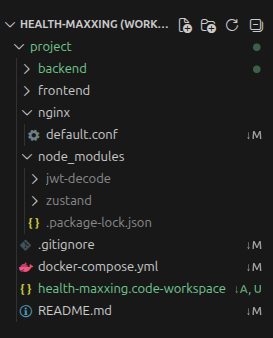
\includegraphics[width=\linewidth]{ScreenshotD3/FoldStruct.png}
            \caption{}
            \label{Folder structure}
        \end{subfigure}
        \hfill \begin{subfigure}[b]{0.32\textwidth}
            \centering
            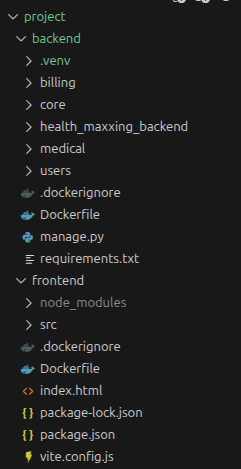
\includegraphics[width=\linewidth]{ScreenshotD3/BE-FE.png}
            \caption{}
            \label{Frontend and Backend}
        \end{subfigure}
        
        \caption{Folder structure, and a on zoom of the frontend and backend (b)}
        \label{Folder stracture, BE-FE}
    \end{figure}
    \FloatBarrier

\end{itemize}
\phantomsection 
% -------------------------------------------------------
\subsection{Language Used and Why}
% -------------------------------------------------------
\phantomsection 
\subsubsection{Frontend Language: JavaScript (React 18.3.1)}

\textbf{Why React?}

\begin{itemize}
  \item \textbf{Reusable Components:} React's component-based architecture allows building modular, reusable UI pieces that reduce code duplication.
  \item \textbf{Flexibility for Routing:} React Router DOM enables client-side routing, allowing seamless navigation without full page reloads.
  \item \textbf{Security Measures:} React provides built-in protections against common vulnerabilities like XSS attacks through automatic escaping.
  \item \textbf{Large Ecosystem:} Extensive community support, libraries, and tools available.
  \item \textbf{Developer Experience:} JSX syntax makes code more readable and maintainable.
\end{itemize}

\textbf{Why NOT Plain HTML/CSS?}

\begin{itemize}
  \item Plain HTML/CSS is considered outdated for modern web applications and not an industry standard.
  \item Lacks dynamic interactivity without extensive custom JavaScript.
  \item No component reusability or state management capabilities.
  \item Poor performance with complex UIs.
\end{itemize}
\phantomsection 
\subsubsection{Backend Language: Python (Django 4.2.30)}

\textbf{Why Django?}

\begin{itemize}
  \item Included as the framework of choice for this project.
  \item Excellent for rapid API development with built-in authentication, ORM, and admin panel.
  \item Strong security features (CSRF protection, SQL injection prevention, etc.).
  \item Well-documented and widely used in production environments.
\end{itemize}
\phantomsection 
% -------------------------------------------------------
\subsection{Database: PostgreSQL}
% -------------------------------------------------------
\phantomsection 
\subsubsection{Why PostgreSQL?}

\begin{itemize}
  \item \textbf{Team Familiarity:} All team members are comfortable with PostgreSQL and the relational database paradigm.
  \item \textbf{Industry Standard:} PostgreSQL is a robust, production-ready relational database trusted by many organizations.
  \item \textbf{Strong Consistency:} ACID compliance ensures data integrity.
  \item \textbf{Advanced Features:} Supports JSON, full-text search, and complex queries out of the box.
\end{itemize}
\phantomsection 
\subsubsection{ER Diagram}

\begin{figure}[htbp]
    \centering
    \includegraphics[width=\textwidth]{ScreenshotD3/ER.png} % Scales to exactly 100% of text width
    \caption{ER diagram}
    \label{fig:large_image}
\end{figure}

\FloatBarrier
\phantomsection 
\subsubsection{Example of some Tables}

\begin{figure}[htbp]
        \centering
        \begin{subfigure}[b]{0.47\textwidth}
            \centering
            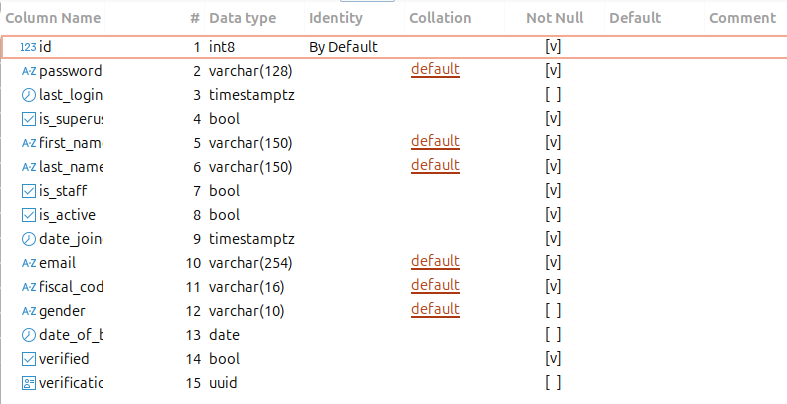
\includegraphics[width=\linewidth]{ScreenshotD3/tableUser.png}
            \caption{}
            \label{User Table}
        \end{subfigure}
        \hfill \begin{subfigure}[b]{0.47\textwidth}
            \centering
            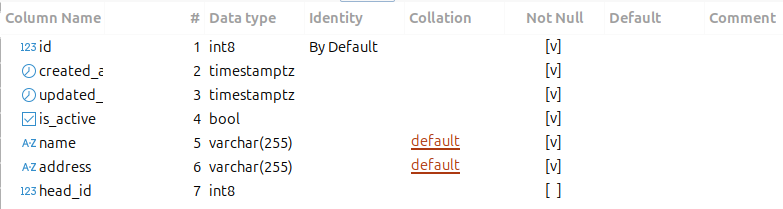
\includegraphics[width=\linewidth]{ScreenshotD3/tableHospital.png}
            \caption{}
            \label{Hospital Table}
        \end{subfigure}
        
        \caption{table of users (a), table of hospitals (b)}
        \label{User and Hospital Tables}
\end{figure}
\FloatBarrier

\phantomsection 
% -------------------------------------------------------
\subsection{Dependencies}
% -------------------------------------------------------
\phantomsection 
\subsubsection{Backend Dependencies}

\begin{longtable}{L{3.6cm} C{2.0cm} L{8.8cm}}
  \rowcolor{tableheader}
  \color{white}\bfseries Dependency &
  \color{white}\bfseries Version &
  \color{white}\bfseries Purpose \\
  \endfirsthead
  \rowcolor{tableheader}
  \color{white}\bfseries Dependency &
  \color{white}\bfseries Version &
  \color{white}\bfseries Purpose \\
  \endhead
  Django & 4.2.30 & Core web framework used to build the backend application and REST API \\
  \rowcolor{tablerowalt}
  Django REST Framework & 3.17.1 & Provides tools for building RESTful APIs, including serialization, authentication, and viewsets \\
  django-cors-headers & 4.9.0 & Handles Cross-Origin Resource Sharing (CORS) between frontend and backend services \\
  \rowcolor{tablerowalt}
  djangorestframework-simplejwt & 5.5.1 & Implements JWT-based authentication for Django REST Framework \\
  PyJWT & 2.13.0 & Creates, signs, decodes, and validates JSON Web Tokens \\
  \rowcolor{tablerowalt}
  psycopg & 3.3.4 & PostgreSQL database adapter for Python \\
  psycopg-binary & 3.3.4 & Pre-compiled PostgreSQL adapter for simplified installation and development \\
  \rowcolor{tablerowalt}
  ruff & 0.15.14 & Python linter and formatter used to enforce code quality standards \\
  asgiref & 3.11.1 & ASGI utilities providing asynchronous support required by Django \\
  \rowcolor{tablerowalt}
  sqlparse & 0.5.5 & SQL parsing library used internally by Django \\
  typing\_extensions & 4.15.0 & Backported and experimental type hinting features for Python \\
  \rowcolor{tablerowalt}
  tzdata & 2026.2 & Time zone database used for accurate date and time handling \\
\end{longtable}
\phantomsection 
\subsubsection{Frontend Dependencies}

\begin{longtable}{L{3.6cm} C{2.0cm} L{8.8cm}}
  \rowcolor{tableheader}
  \color{white}\bfseries Dependency &
  \color{white}\bfseries Version &
  \color{white}\bfseries Purpose \\
  \endfirsthead
  \rowcolor{tableheader}
  \color{white}\bfseries Dependency &
  \color{white}\bfseries Version &
  \color{white}\bfseries Purpose \\
  \endhead
  React & 18.3.1 & Core UI library for building interactive components \\
  \rowcolor{tablerowalt}
  react-dom & 18.3.1 & Renders React components to the DOM \\
  react-router-dom & 6.0.0 & Client-side routing for seamless page navigation \\
  \rowcolor{tablerowalt}
  Vite & 5.4.1 & Lightning-fast build tool and dev server (modern webpack alternative) \\
  @vitejs/plugin-react & 4.3.1 & Vite plugin for React support with Fast Refresh \\
  \rowcolor{tablerowalt}
  zustand & 5.0.14 & Lightweight state management library for global application state, including authentication data \\
  jwt-decode & 4.0.0 & Decodes JWT tokens on the client side to extract user information and token claims without server requests \\
\end{longtable}
\phantomsection 
\subsubsection{Infrastructure Dependencies}

\begin{longtable}{L{3.6cm} L{10.8cm}}
  \rowcolor{tableheader}
  \color{white}\bfseries Dependency &
  \color{white}\bfseries Purpose \\
  \endfirsthead
  \rowcolor{tableheader}
  \color{white}\bfseries Dependency &
  \color{white}\bfseries Purpose \\
  \endhead
  Nginx & Reverse proxy server for routing requests, serving static assets, and load balancing \\
  \rowcolor{tablerowalt}
  Docker & Containerization platform for consistent development, testing, and production environments \\
  docker-compose & Orchestrates multi-container Docker applications (frontend, backend, database) \\
\end{longtable}

\textbf{Why These Infrastructure Tools?}

\begin{itemize}
  \item \textbf{Nginx:} Acts as a reverse proxy, routing frontend requests to the React app and API requests to Django. Improves performance and security.
  \item \textbf{Docker:} Ensures the application runs consistently across all environments (local, CI/CD, production). Eliminates ``works on my machine'' problems.
  \item \textbf{docker-compose:} Simplifies local development by defining and running all services (frontend, backend, database) in one configuration file.
\end{itemize}
\phantomsection 
% -------------------------------------------------------
\subsection*{Summary}
% -------------------------------------------------------

\begin{tabular}{L{2.6cm} L{3.4cm} L{7.4cm}}
  \rowcolor{tableheader}
  \color{white}\bfseries Component &
  \color{white}\bfseries Choice &
  \color{white}\bfseries Reason \\
  Architecture & 3-Tier & Maintainability, separation of duties, scalability \\
  \rowcolor{tablerowalt}
  Frontend & React 18 + Vite & Reusable components, flexible routing, security, modern tooling \\
  Backend & Django + DRF & Rapid API development, built-in security, ORM, admin panel \\
  \rowcolor{tablerowalt}
  Database & PostgreSQL & Team familiarity, relational paradigm, ACID compliance, industry standard \\
  Infrastructure & Docker + Nginx & Consistency, reverse proxy, containerization, ease of deployment \\
\end{tabular}

\newpage
\phantomsection 
\section{Use Cases Implemented}
During the implementation phase the goal was to cover the main functionalities of the app, with special focus on the management of the hierarchical hospital structure, giving the system administrator all the tools necessary to manage such structure.

In particular, we implemented the use cases:

\begin{enumerate}
    \item \textbf{UC1} - Create Treatment / Hospital / Department DONE
    \item \textbf{UC2} - Create Insurance Policy DONE
    \item \textbf{UC5} - Edit Treatment / Hospital / Department DONE
    \item \textbf{UC6} - Update Insurance Policy    DONE
    \item \textbf{UC8} - Deactivate or close Treatment / Hospital / Department  DONE
    \item \textbf{UC9} - Deactivate Insurance Policy    DONE
    \item \textbf{UC10} - Cancel Appointment (Patient) DONE
    \item \textbf{UC12} - Register Doctor
    \item \textbf{UC13} - Assign Doctor to Hospital
    \item \textbf{UC14} - Appoint Head of Hospital
    \item \textbf{UC15} - Appoint Head of Department
    \item \textbf{UC16} - Assign Doctor to Department
    \item \textbf{UC22} - Generate Insurancce Policy Code
    \item \textbf{UC23} - User Registration and Validation -  Cambiare nome UC (riguarda solo patient)
    \item \textbf{UC24} - User Login 
    \item \textbf{UC25} - Automated Doctor Assignment
    \item \textbf{UC27} - Appointment Booking
    \item \textbf{UC28} - Appointment View - partial
    \item \textbf{UC29} - Appointment Rescheduling
\end{enumerate}


\phantomsection 
\section{User Flows}
This section of the document covers the user flows regarding most of the use cases. The user flows are divided by actor and for each actor first appear those that have been implemented, followed by those that have not been implemented.
In order to simplify user flows and ease understanding, some general flows such as "Fill Form" were created. Such flows are described at the beginning of the document, shown entirely within the first user flow that makes use of them and the simply referred to in the rest of the user flows. Moreover - in the user flows covering multiple use cases - the use case that a particular branch covers is written in the transition arrow.

\phantomsection 
\subsection{Diagram Legend}
The User Flows make use of different shapes and colors, each with an associated meaning. In particular:
\begin{itemize}
    \item \textbf{Lightblue Ellipse: }Used to represent the start, end or stop of the User Flows, "Start" refers to the beginning of the flow, "End" to the successful completion of the user flow (i.e. the end of the happy path) and "Stop" refers to the unsuccesful end of the flow, caused by some error. Moreover "Continue" is used in general flows to specify where the next step of a User Flow incuding a general flow will be.
    \item \textbf{Green Rounded Rectangle: }Used to represent the states of the interface (i.e. what an actor sees at some point in the flow).
    \item \textbf{Yellow Diamond: }Used to represent the decisions in the User Flows and the choiche of page from the Navbar.
    \item \textbf{Red Rounded Rectangle: }Used to represent the actions in the User Flows.
    \item \textbf{Pink Roundend Rectangle: }Used to represent general flows (e.g., "Fill Form"), which are described in detail at the beginning of the document. When inserting a general flow into a larger diagram, the following logic applies:
        \begin{enumerate}
            \item The pink rounded rectangle must be preceded by an interface state (e.g., "Registration Form").
            \item This interface state represents the first step of the general flow.
            \item The step immediately following the general flow replaces the "Continue" lightblue ellipse from the base diagram.
        \end{enumerate}
\end{itemize}

\newpage
\phantomsection 
\subsection{Actors}
The actors are:
\begin{itemize}
    \item \textbf{User:} This actor represents a general user who could be a Patient, Doctor, Head of Hospital or Head of Department. A User's main functionalities cover registration, login, calendar view and profile managment.
    \item \textbf{Admin:} This actor represents the system administrator, whose main activities cover the management of the hospital structure.
    \item \textbf{Patient:} This actor represents a patient within the healtcare system, whose main functionalities regard the booking and management of appointments.
    \item \textbf{Doctor:} This actor represents a general doctor within a healtcare system, including Head of Hospital and Head of Department. A Doctor's main functionalities regard the management and tracking of examinations and the consultations of Patients' medical records.
    \item \textbf{Head of Hospital:} This actor represents a specific doctor who was appointed as the head of a hospital, whose main fuctionalities regard the management of an hospital facility
    \item \textbf{Head of Department:} This actor represents a specific doctor who was appointed as the head of a department, whose main functionalieties regard the management of a department within an hospital facility.
\end{itemize}
% --- eg ---
\newpage
\begin{minipage}{\textwidth}
    \phantomsection 
    \subsection{General Flow - Fill Form Flow}
    The following diagram describes in detail the steps of the general Fill Form flow, expandend in the user flow  \hyperref[UF12]{UF12. Patient - Registration and Validation}.
    
    \begin{center}
        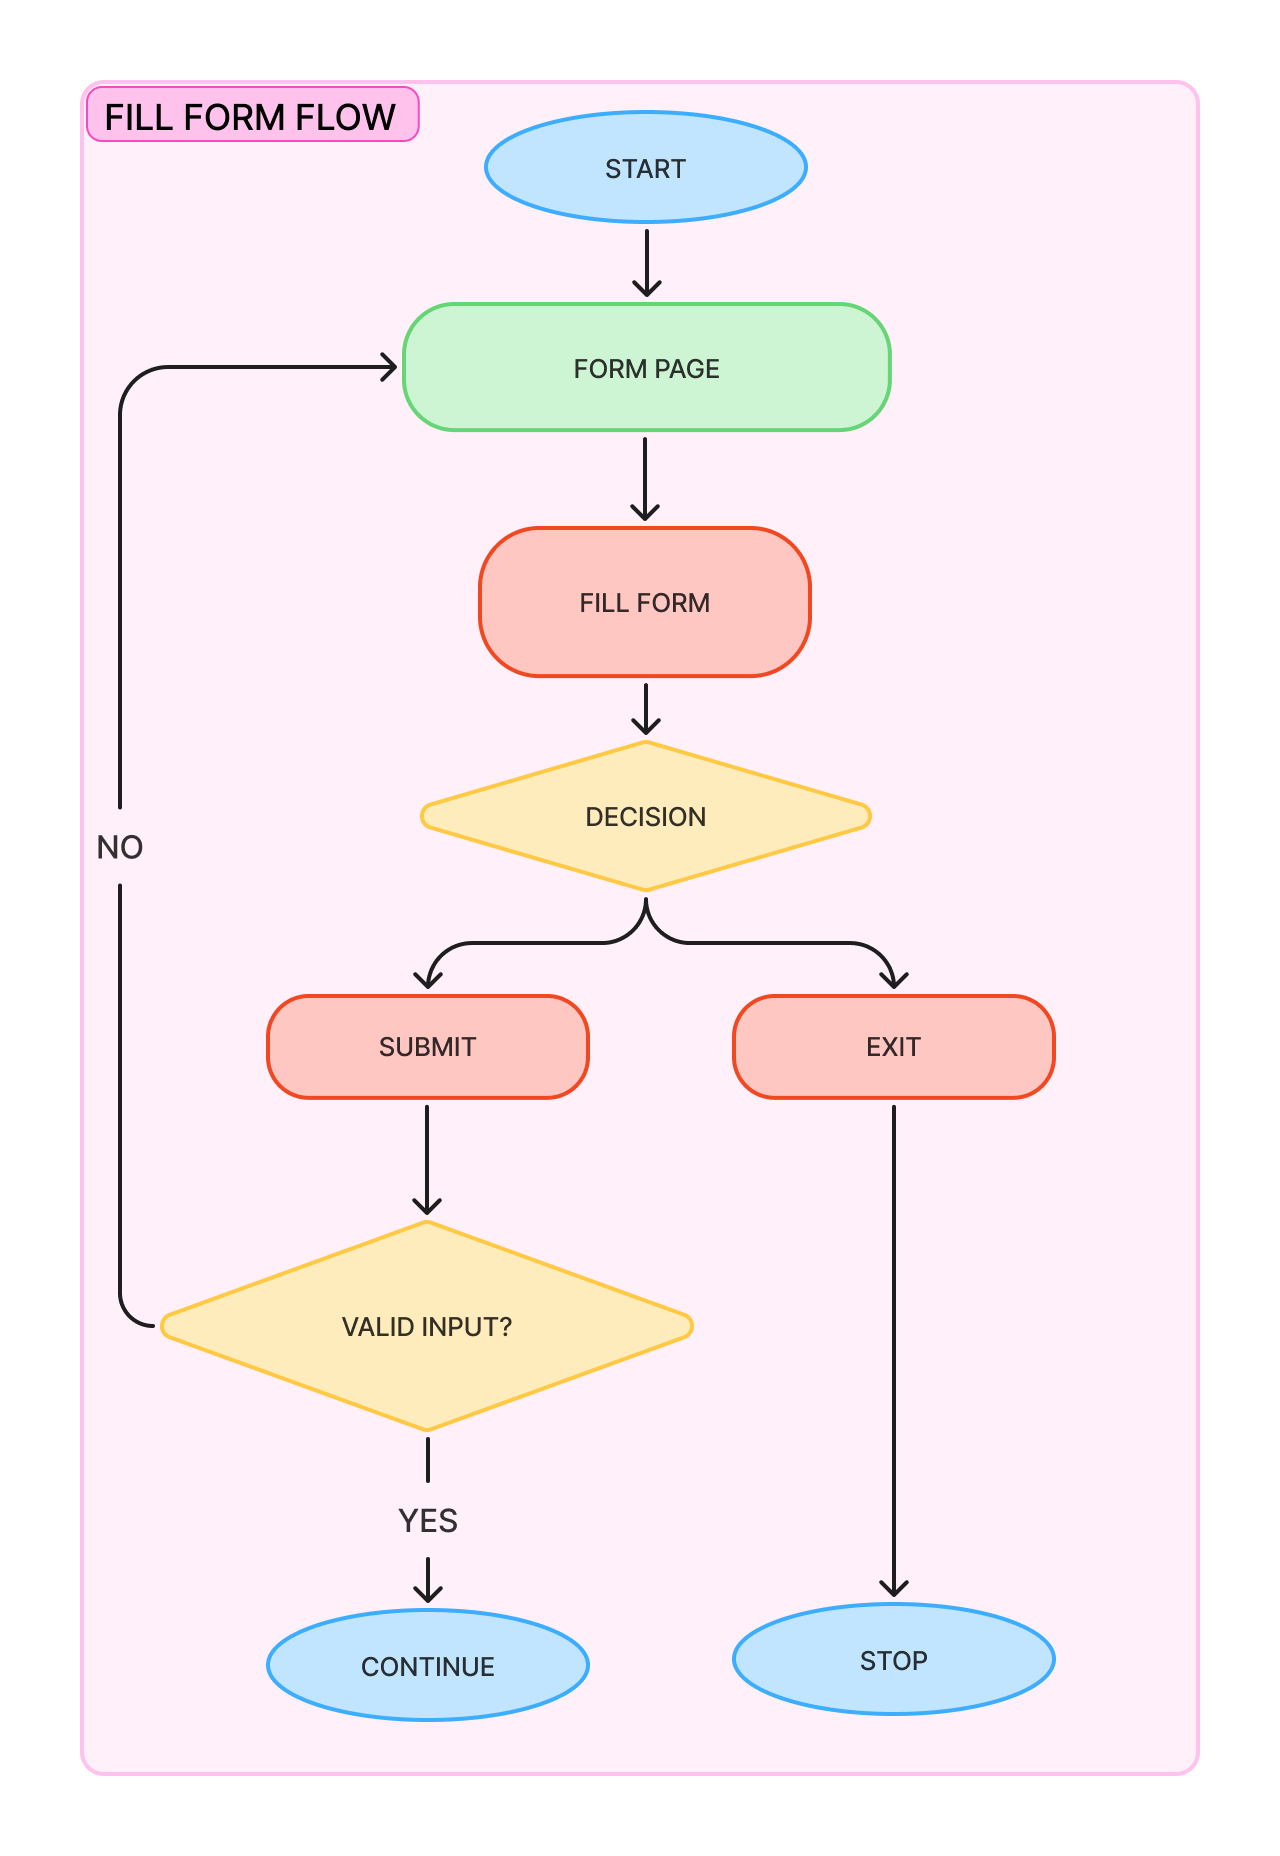
\includegraphics[width=8cm]{User_Flows/FillForm.png}
        \captionof{figure}{General Fill Form Flow}
    \end{center}
    %\begin{itemize}   
    %\end{itemize}
\end{minipage}
\vspace{3em}

\begin{minipage}{\textwidth}
    \phantomsection 
    \subsection{General Flow - Detailed Access Flow}
    The following diagram describes in detail the steps of the general Detailed Access flow, expandend in the user flow \hyperref[UF15]{UF15. Patient - Medical Record and Prescriptions consultation}.
    
    \begin{center}
        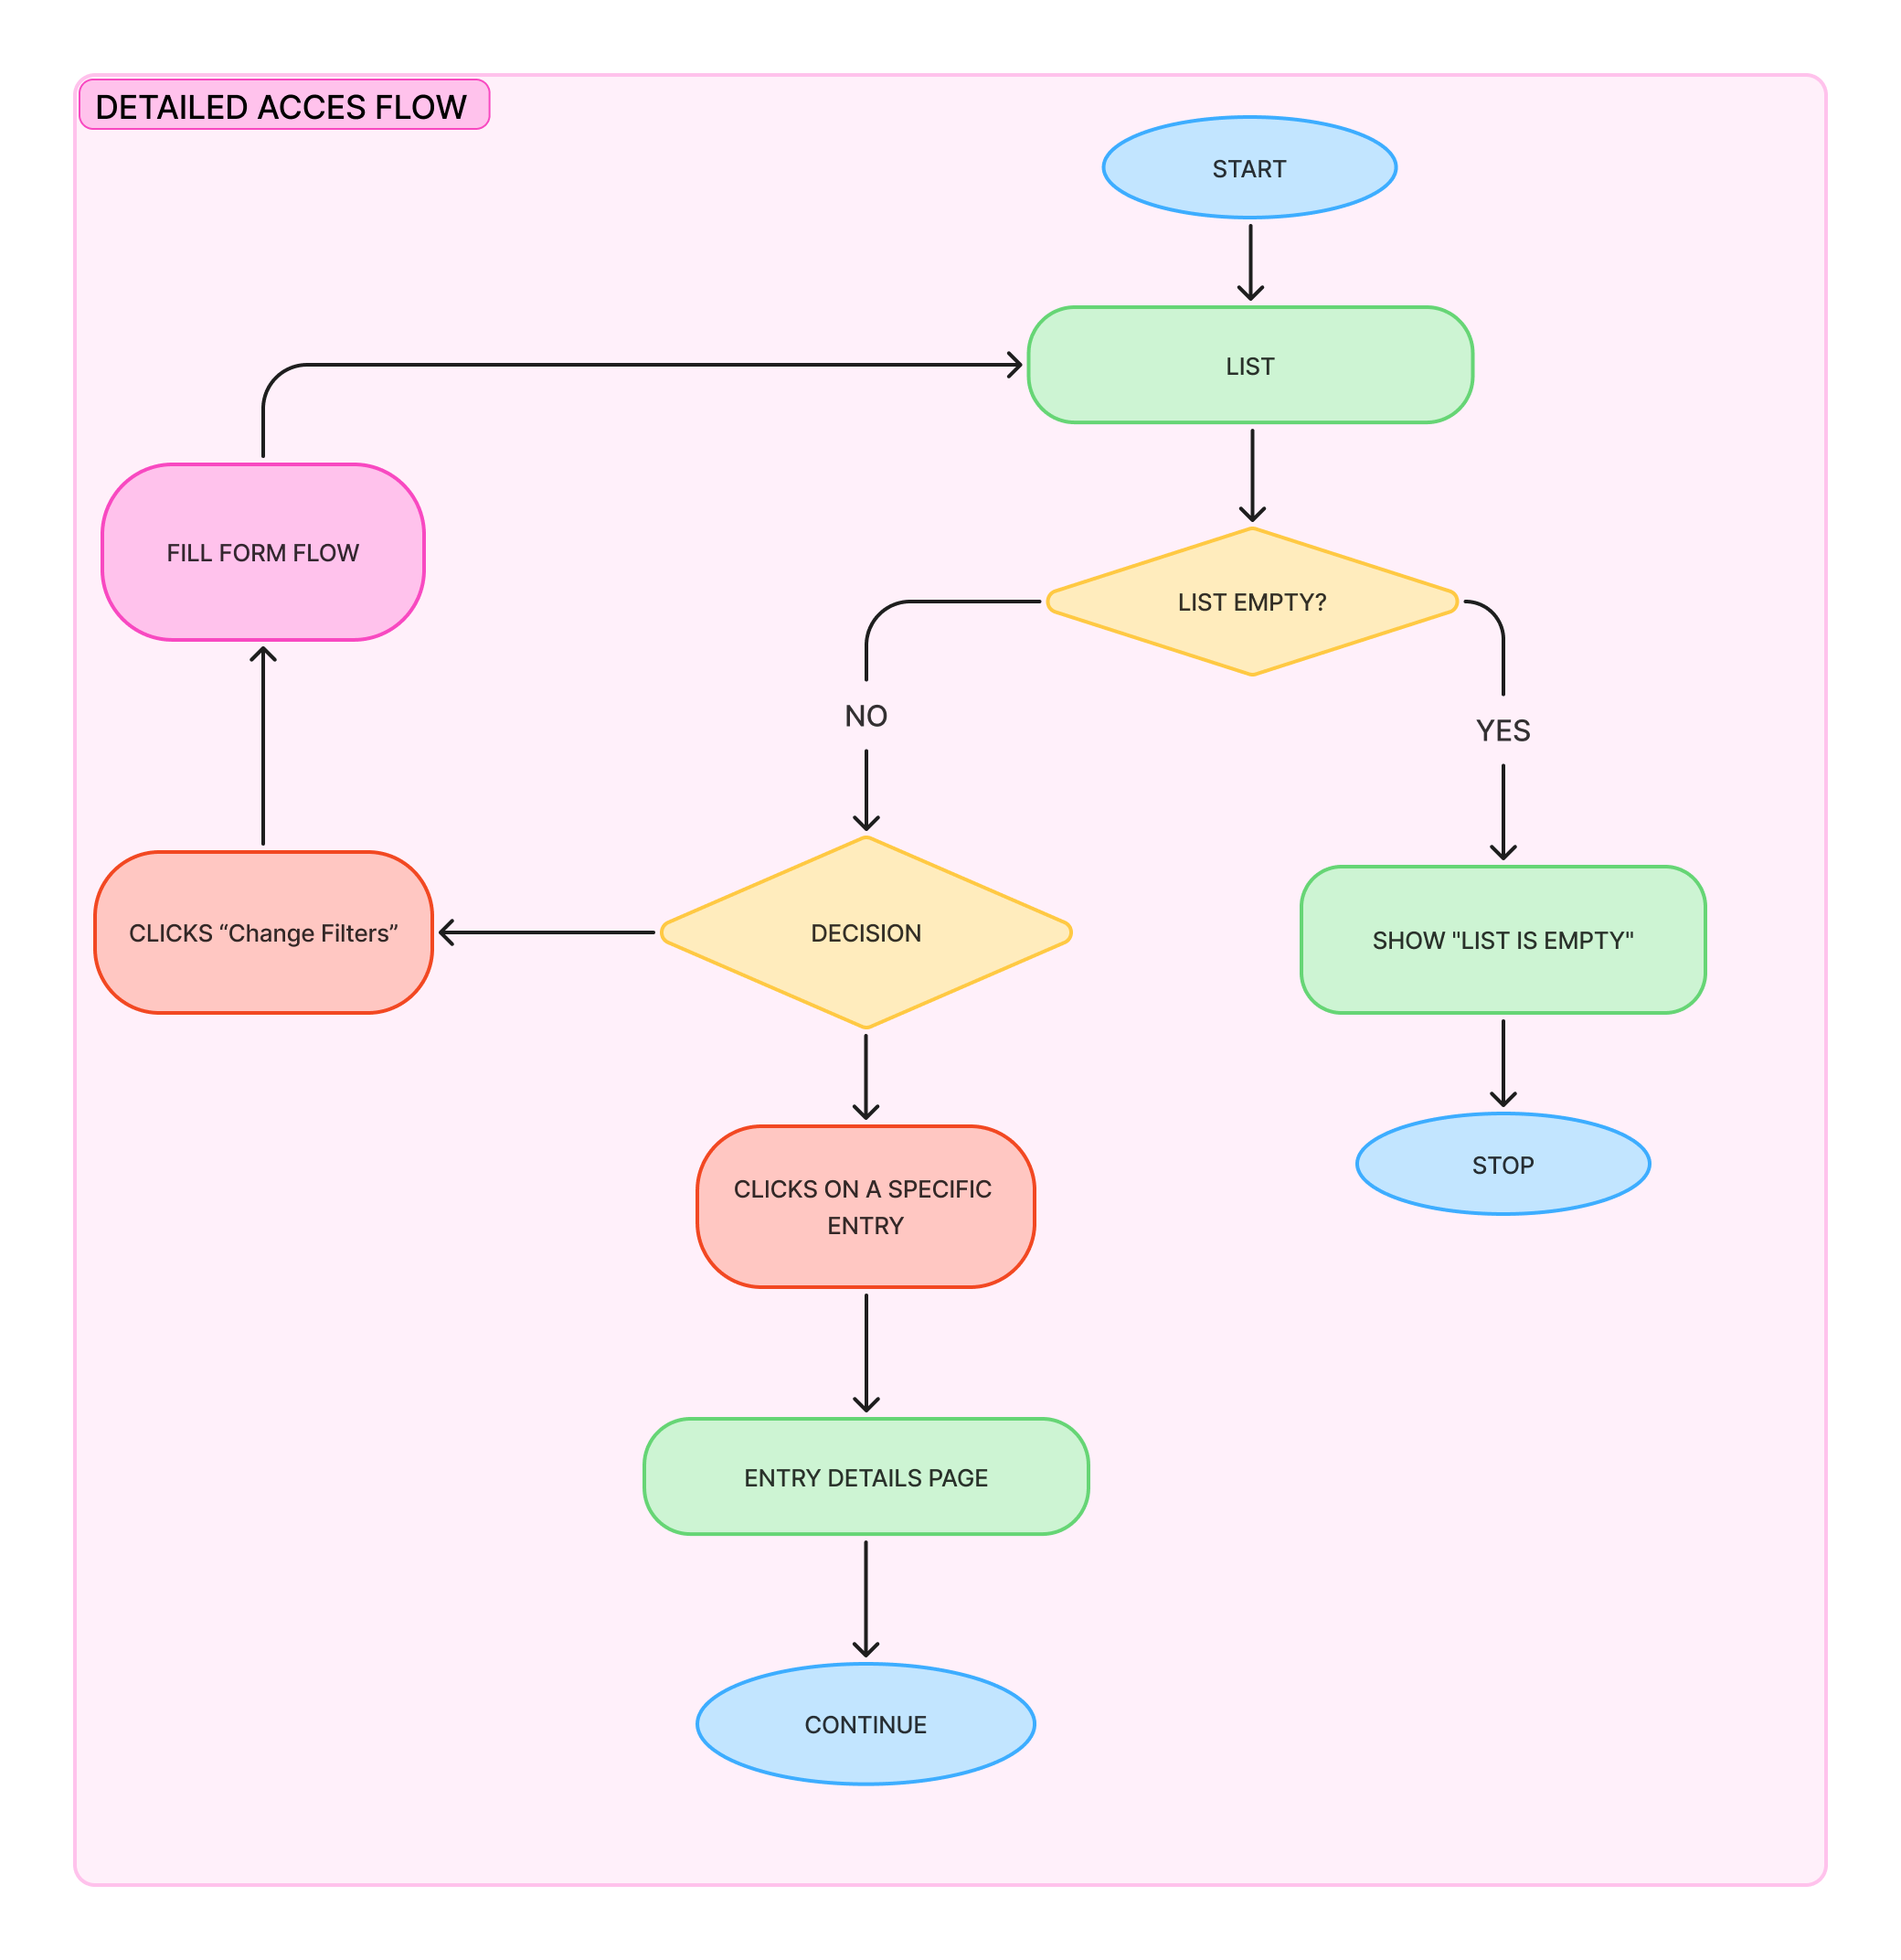
\includegraphics[width=9cm]{User_Flows/DetailedAccess.png}
        \captionof{figure}{General Detailed Access Flow}
    \end{center}
    %\begin{itemize}   
    %\end{itemize}
\end{minipage}
\vspace{3em}

\begin{minipage}{\textwidth}
    \phantomsection 
    \subsection{General Flow - Creation Flow}
    The following diagram describes in detail the steps of the general Creation flow, expandend in the user flow \hyperref[UF6]{UF6. Admin - Create Insurance Policy, Hospital, Treatment, Department. Register Doctor}.
    
    \begin{center}
        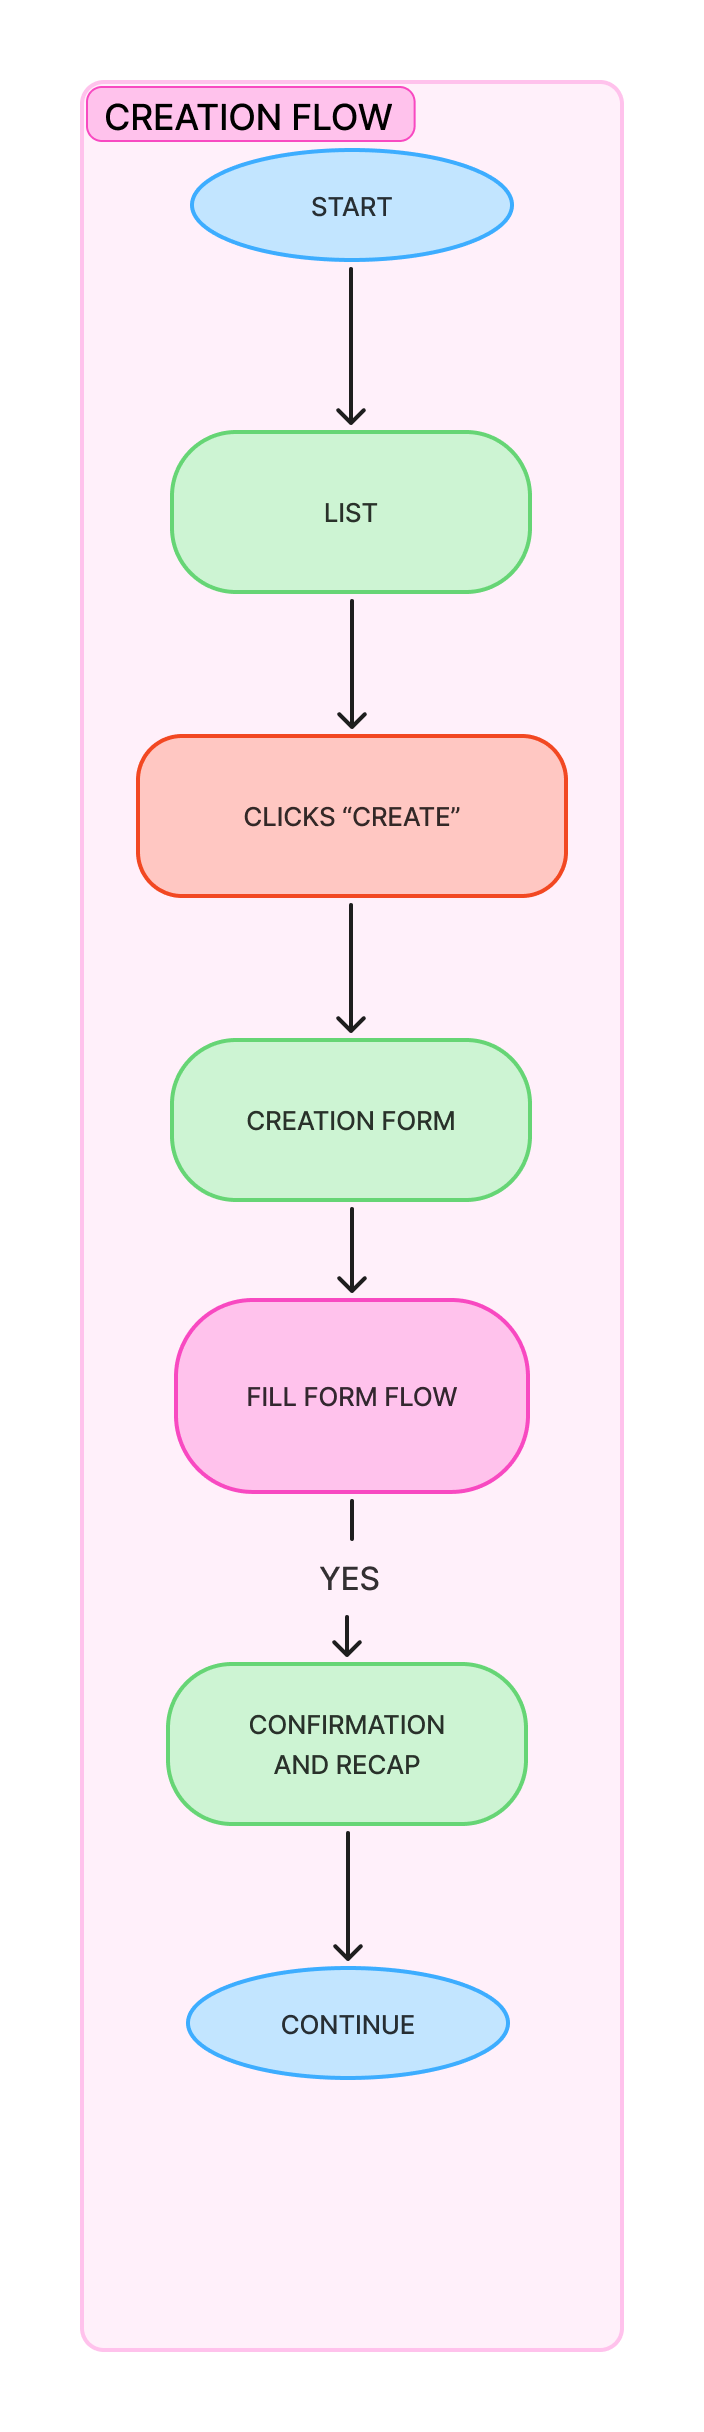
\includegraphics[width=5cm]{User_Flows/Creation.png}
        \captionof{figure}{General Creation Flow}
    \end{center}
    %\begin{itemize}   
    %\end{itemize}
\end{minipage}
\vspace{3em}

\begin{minipage}{\textwidth}
    \phantomsection
    \subsection{General Flow - Edit Flow}
    The following diagram describes in detail the steps of the general Edit flow, expanded in the user flow \hyperref[UF7]{UF7. Admin - Edit Insurance Policy, Hospital, Treatment, Department. Register Doctor}.
    In order to simplify the diagram
    \begin{center}
        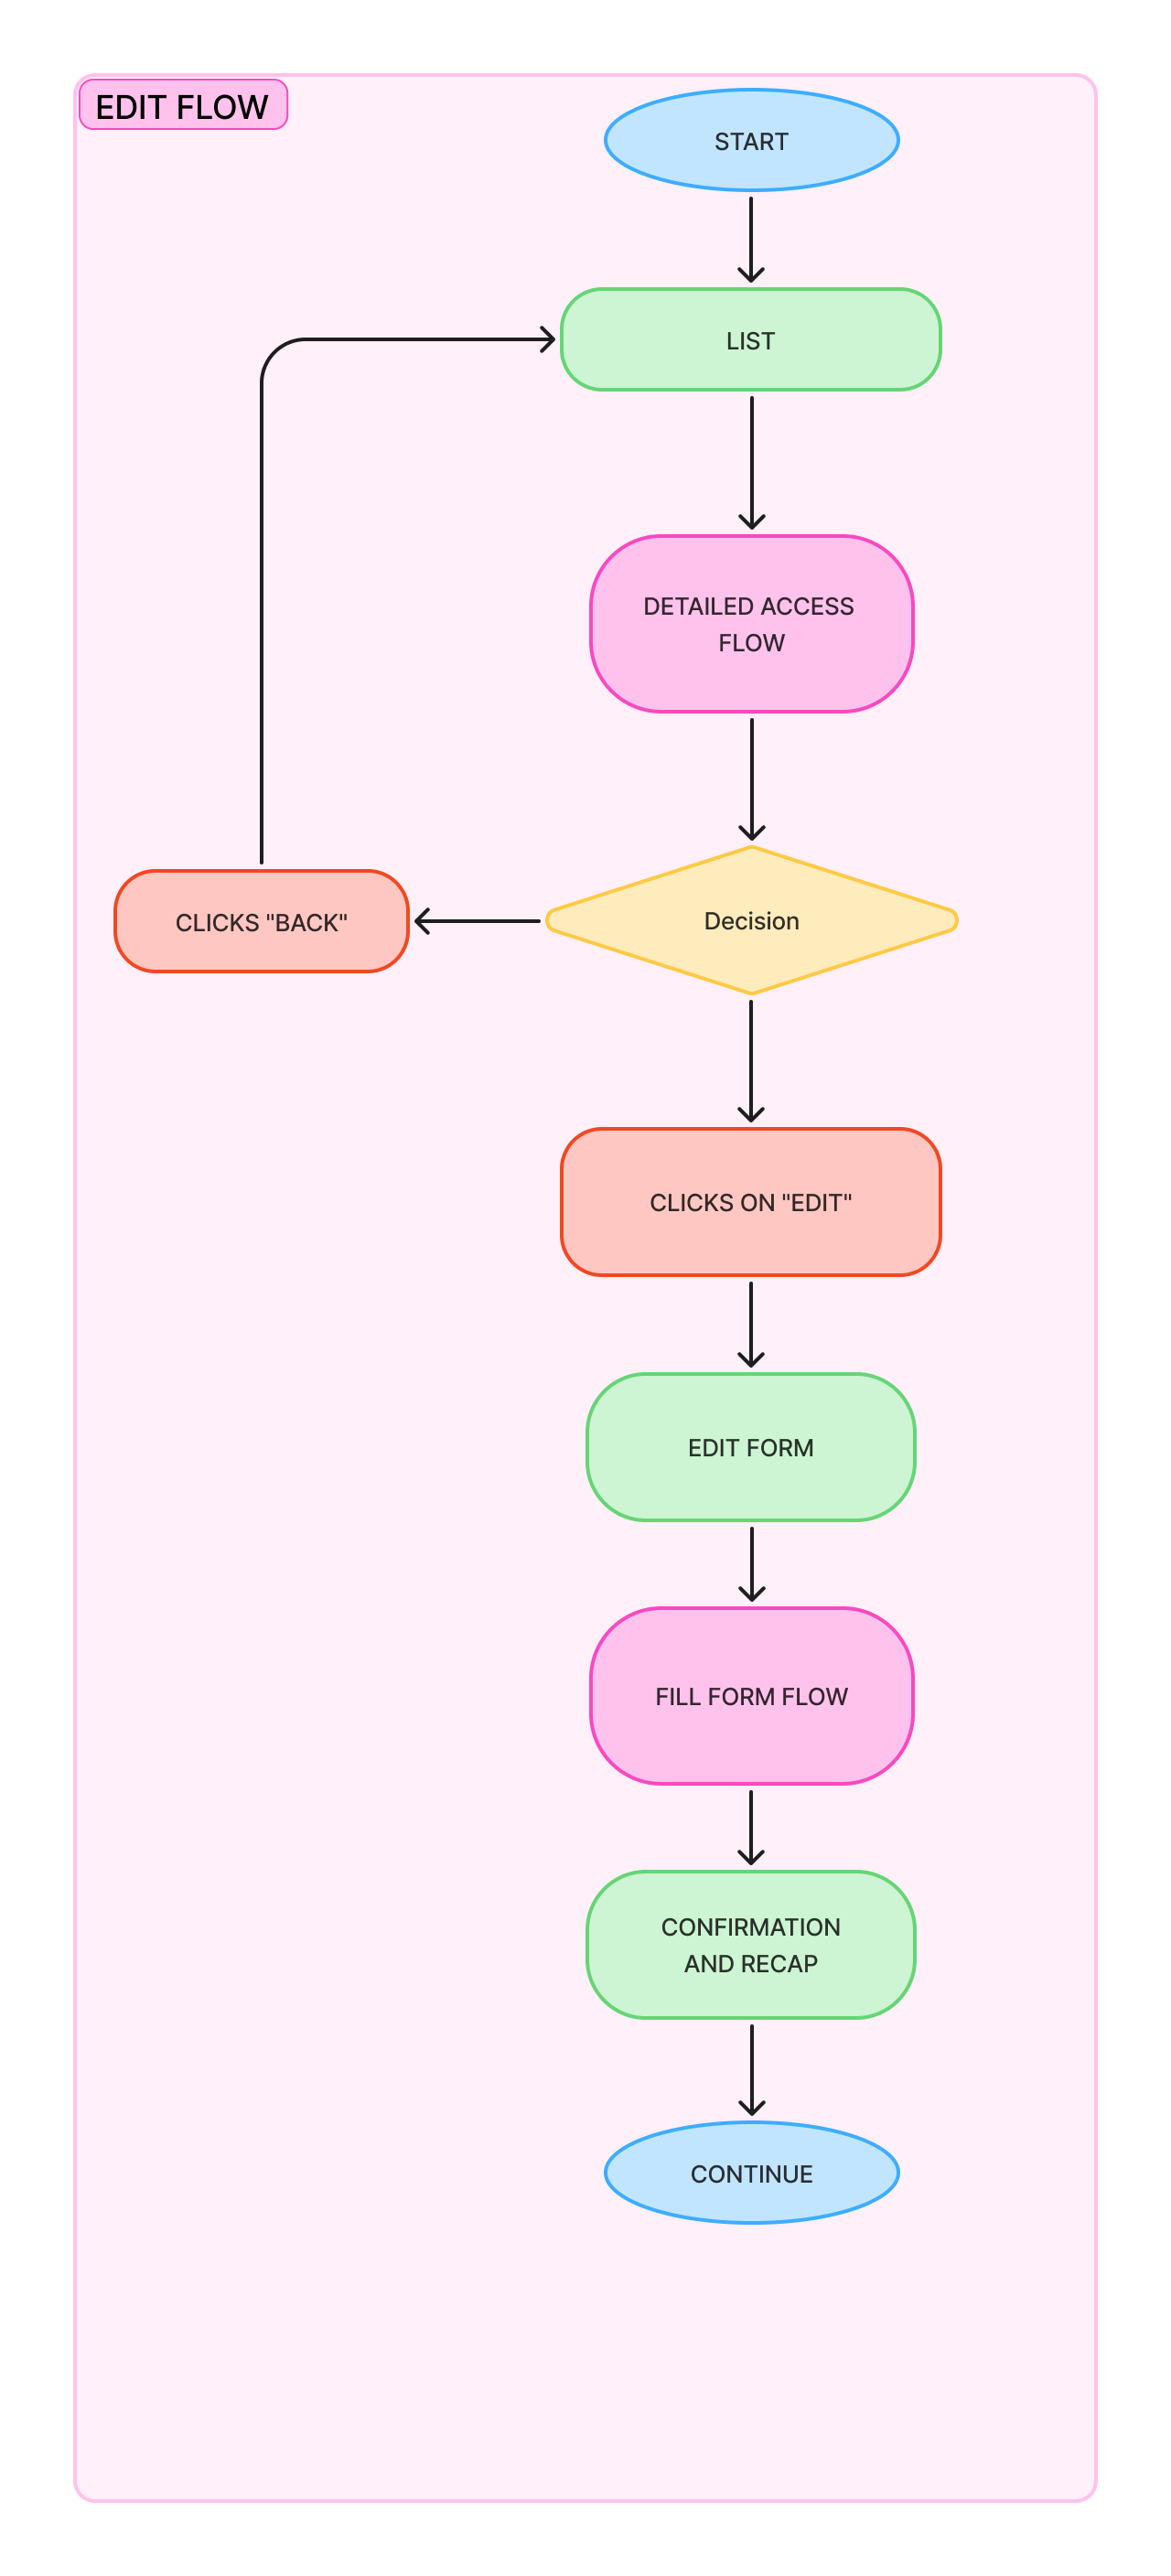
\includegraphics[width=8cm]{User_Flows/Edit.png}
        \captionof{figure}{General Edit Flow}
    \end{center}
    %\begin{itemize}   
    %\end{itemize}
\end{minipage}
\vspace{3em}

\begin{minipage}{\textwidth}
    \phantomsection
    \subsection{General Flow - Deletion Flow}
    The following diagram describes in detail the steps of the general Deletion flow, expanded in the user flow \hyperref[UF8]{UF8. Admin - Deactivate Insurance Policy, Hospital, Treatment, Department}.
    
    \begin{center}
        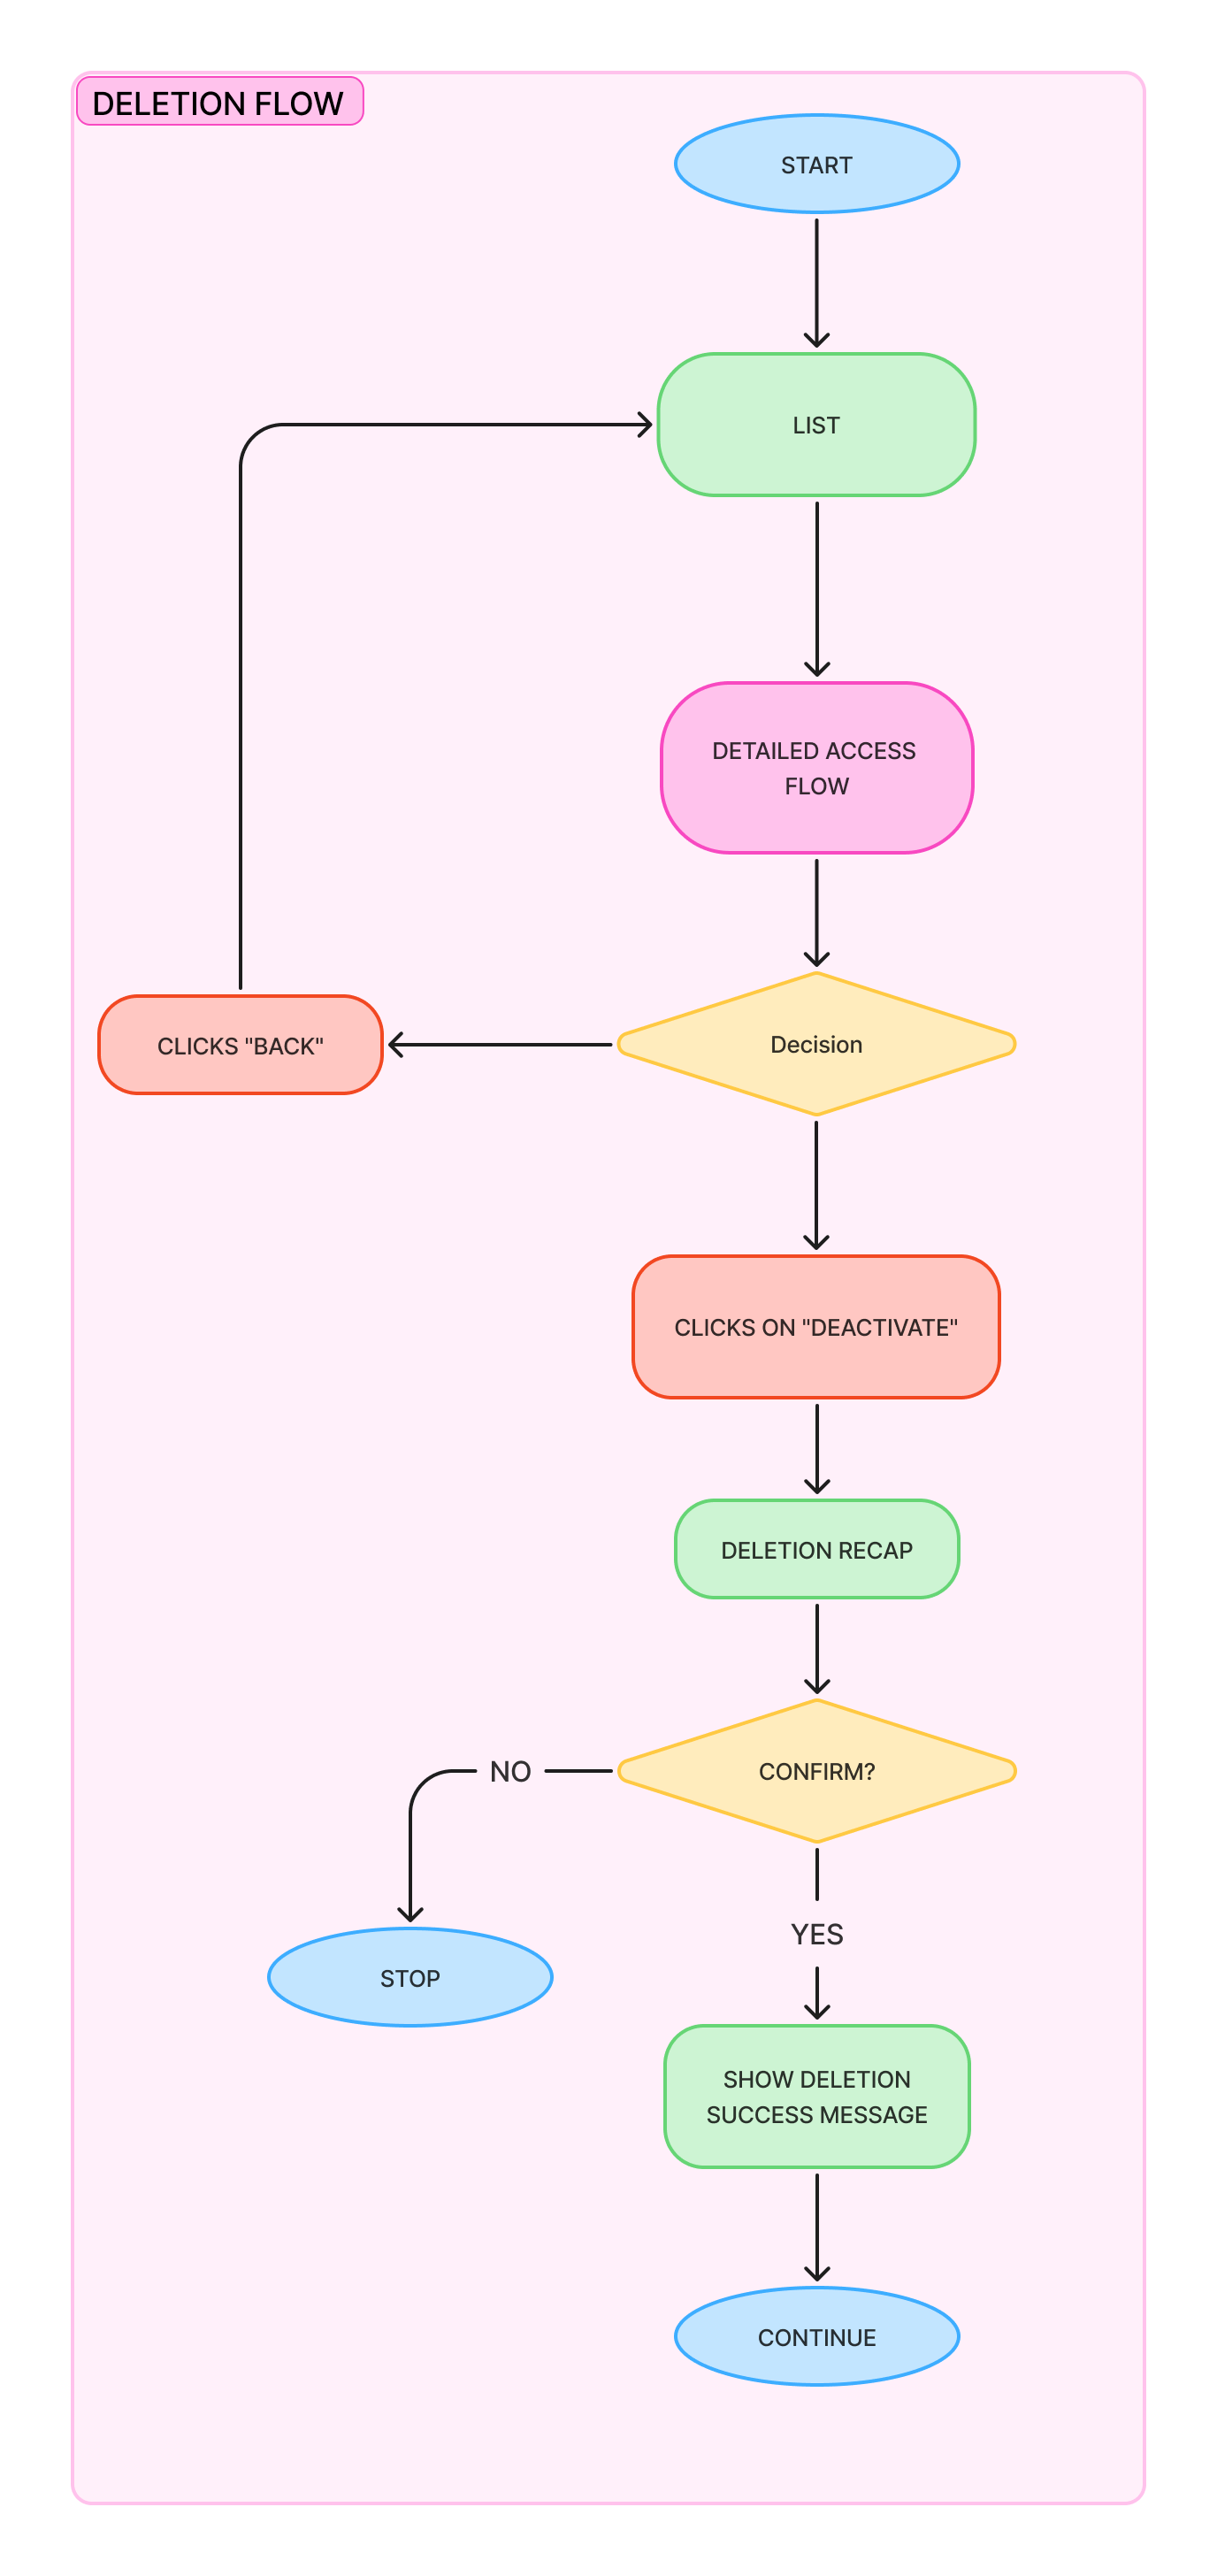
\includegraphics[width=8cm]{User_Flows/Deletion.png}
        \captionof{figure}{General Deletion Flow}
    \end{center}
    %\begin{itemize}   
    %\end{itemize}
\end{minipage}
\vspace{3em}

\begin{minipage}{\textwidth}
    \phantomsection
    \subsection{UF1. User - Login and Recovery}
    The following user flow shows the process of User login and account recovery.
    It refers to use cases \textbf{UC24, UC26}, and methods \textbf{login(), requestPasswordReset()} from the class \textbf{User} of the class diagram.
    
    \begin{center}
        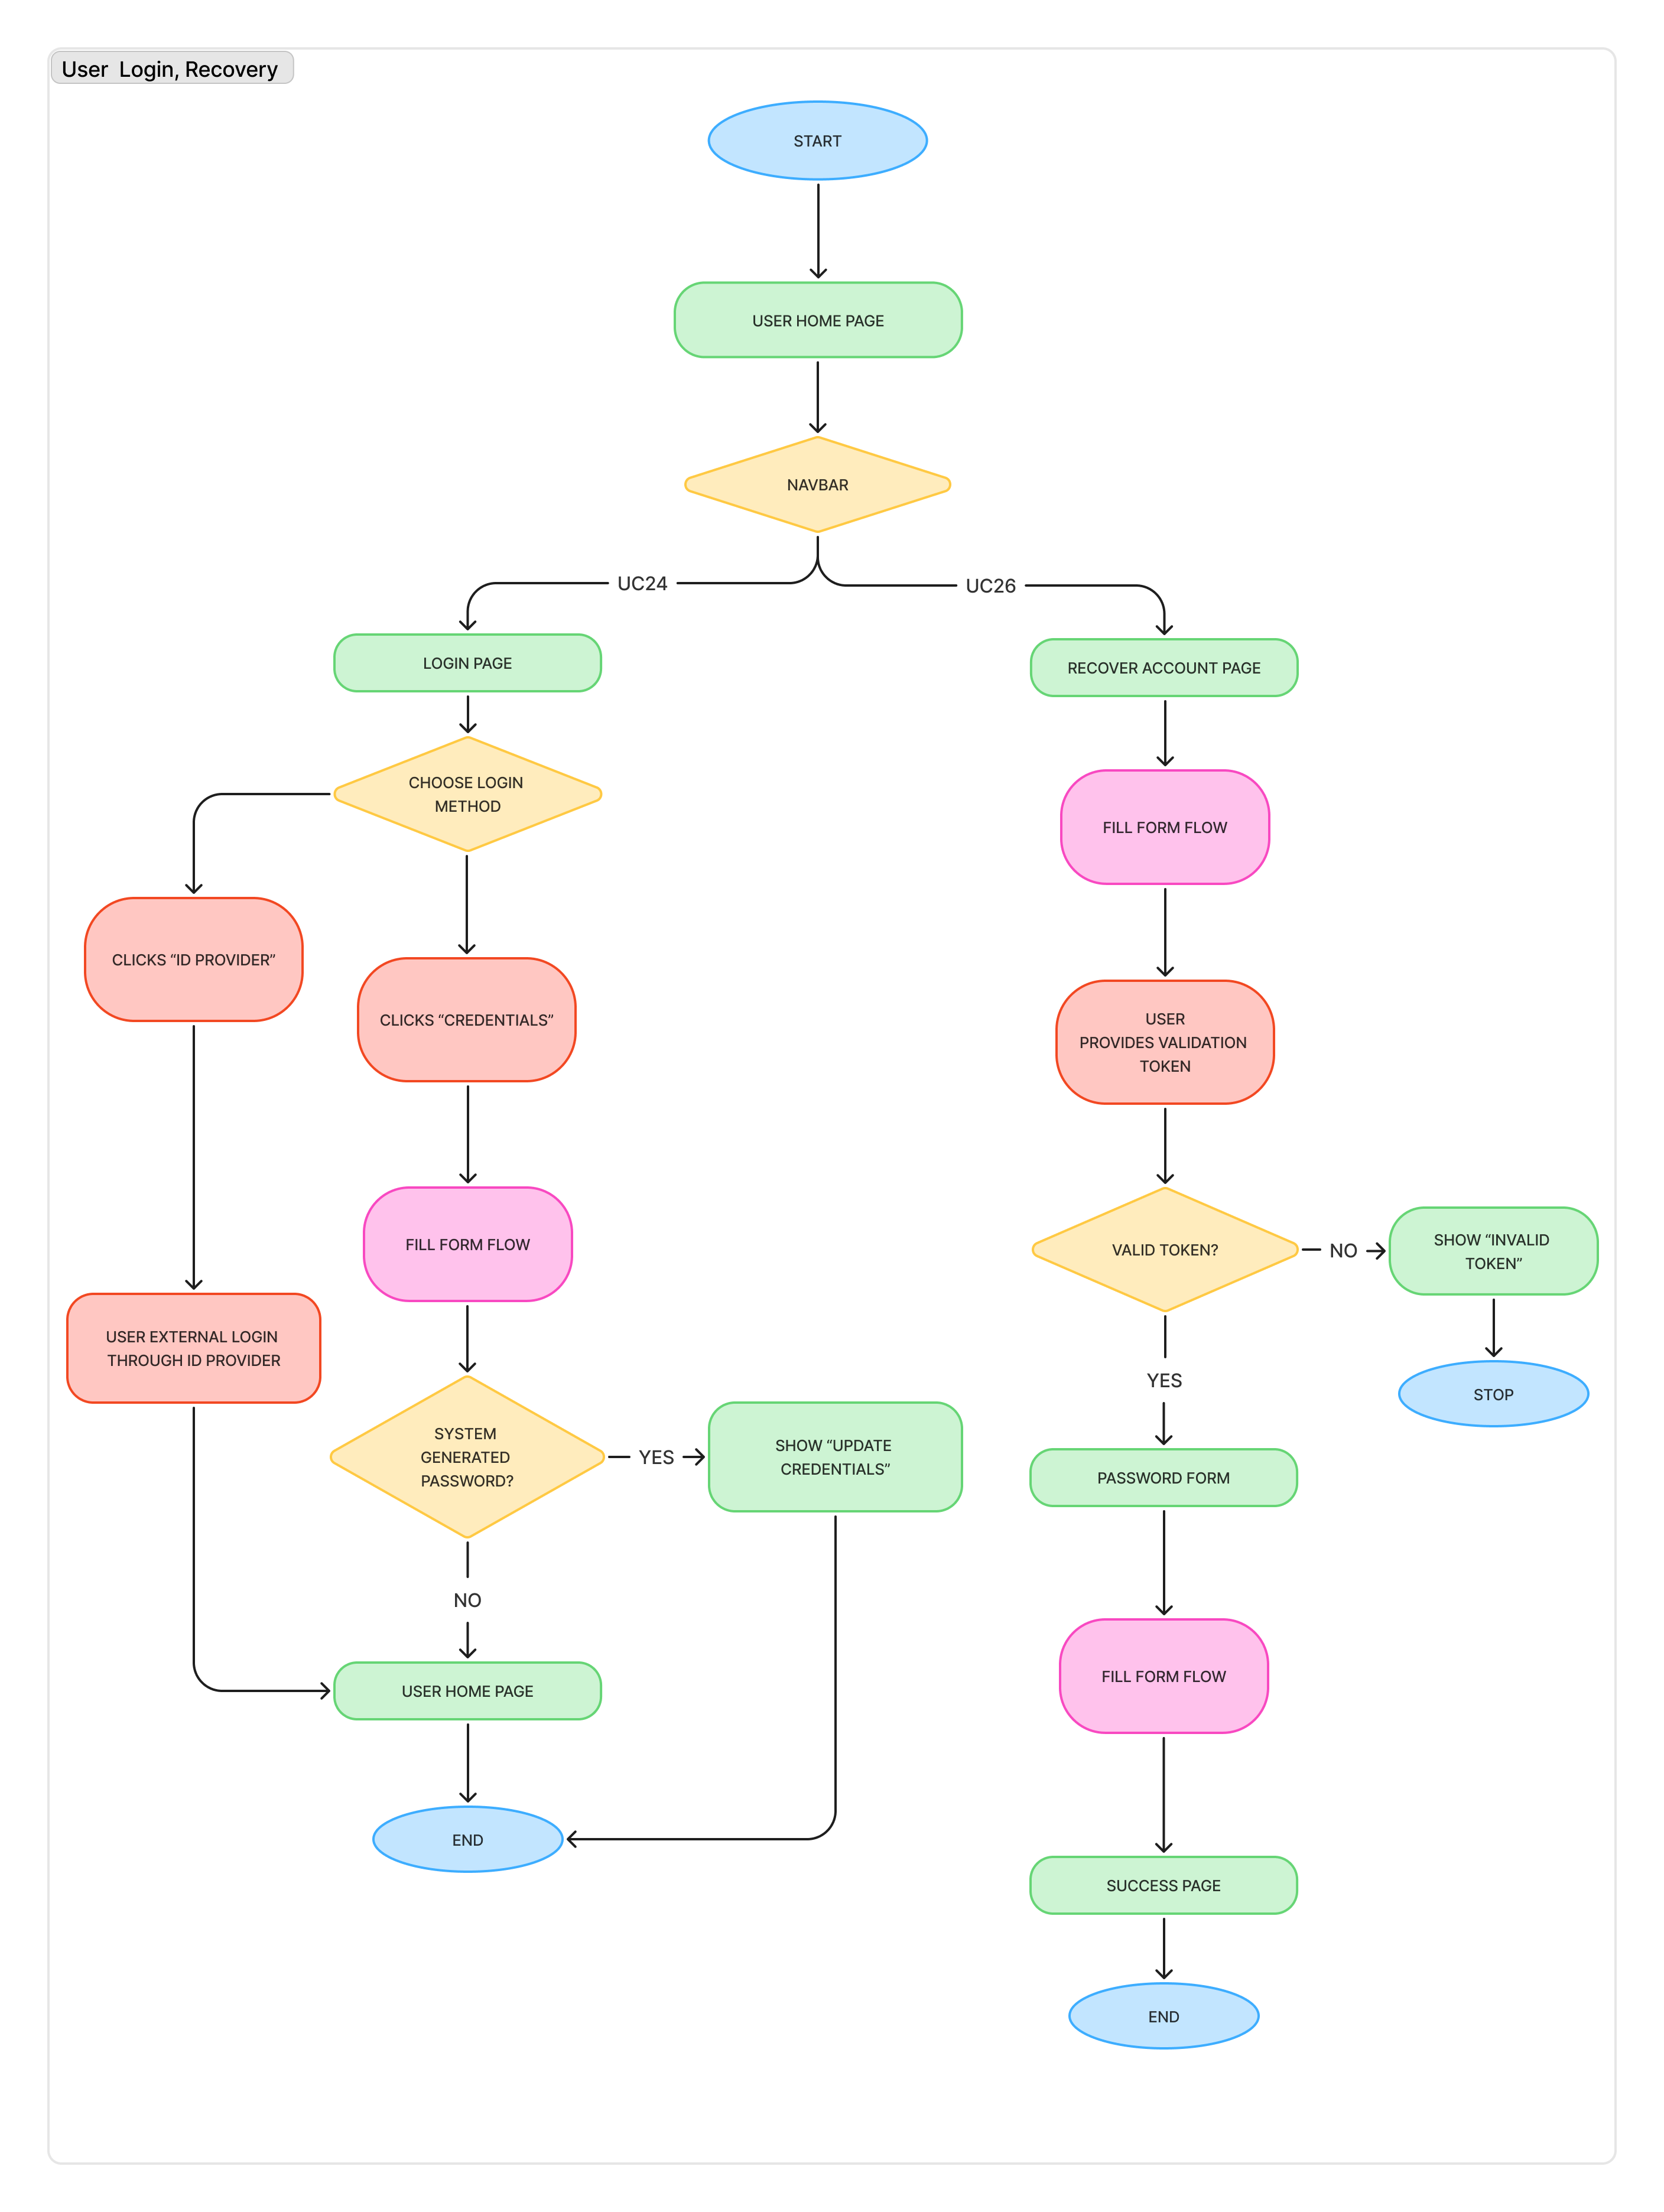
\includegraphics[width=0.8\textwidth]{User_Flows/LoginRecovery.png}
        \captionof{figure}{User flow regarding User Login and Recovery}
    \end{center}
    %\begin{itemize}   
    %\end{itemize}
\end{minipage}
\vspace{3em}


\begin{minipage}{\textwidth}
    \phantomsection
    \subsection{UF2. User - Internal Calendar}
    The following user flow shows the steps a user takes to view their calendar and see the detailes of a booked appointment.
    It refers to use cases \textbf{UC30, UC28}, and methods \textbf{??, ??} from the class \textbf{User} of the class diagram.
    
    \begin{center}
        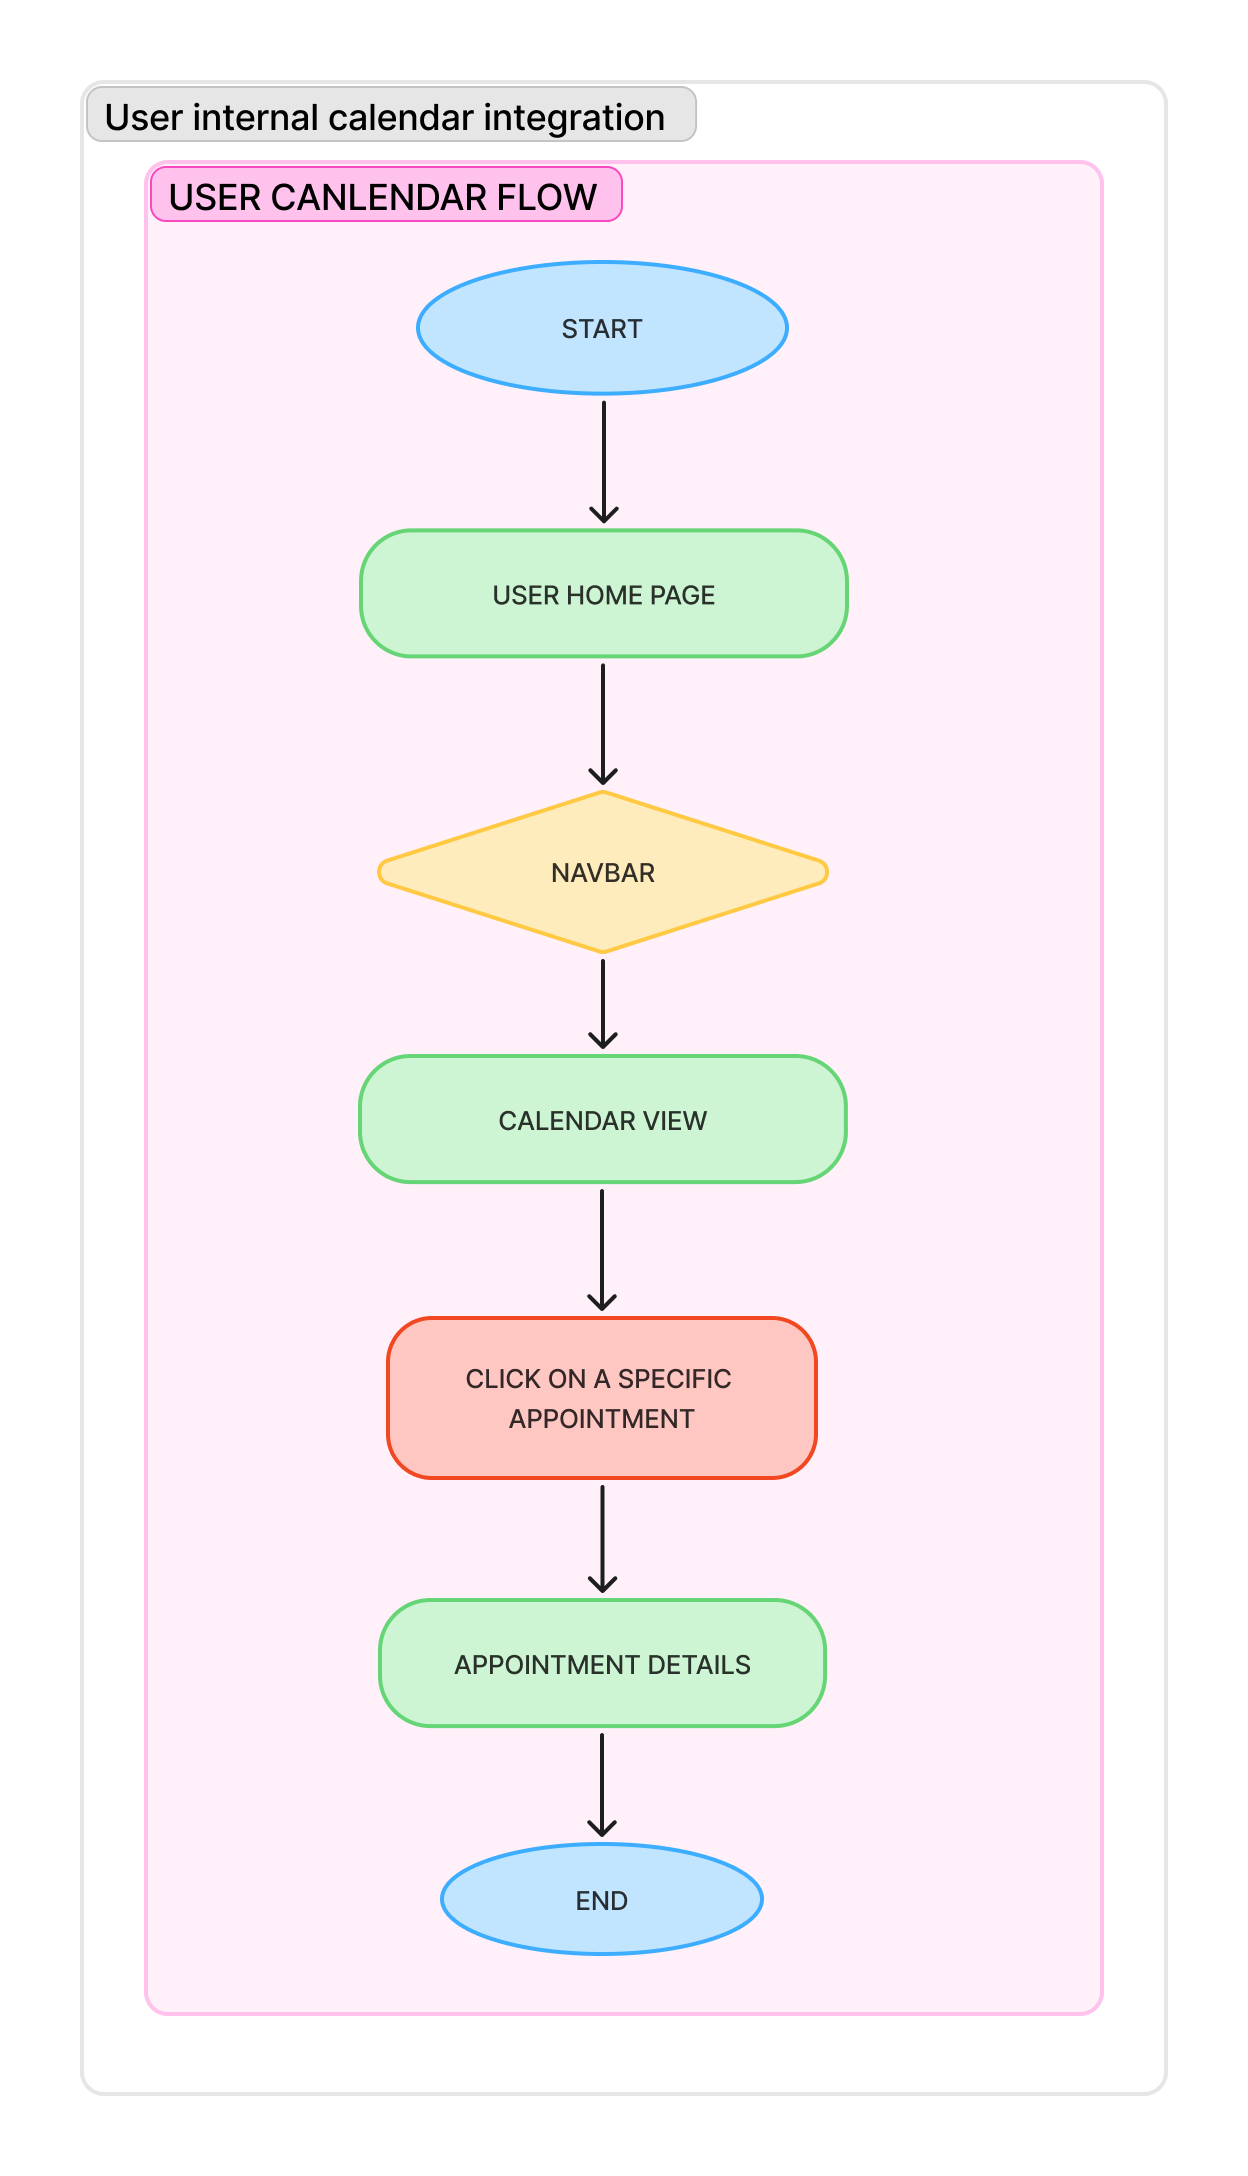
\includegraphics[width=8cm]{User_Flows/UserInternalCalendar.png}
        \captionof{figure}{User flow regarding Internal Calendar integration and View Appointment Details}
    \end{center}
    %\begin{itemize}   
    %\end{itemize}
\end{minipage}
\vspace{3em}


\begin{minipage}{\textwidth}
    \phantomsection
    \subsection{UF3. User - Profile Update and Deletion}
    The following user flow shows the steps a user takes to update and delete their profile.
    It refers to use cases \textbf{UC7, UC41}, and methods \textbf{viewProfile(), updateProfile(), deleteAccount()} from the class \textbf{User} of the class diagram.
    
    \begin{center}
        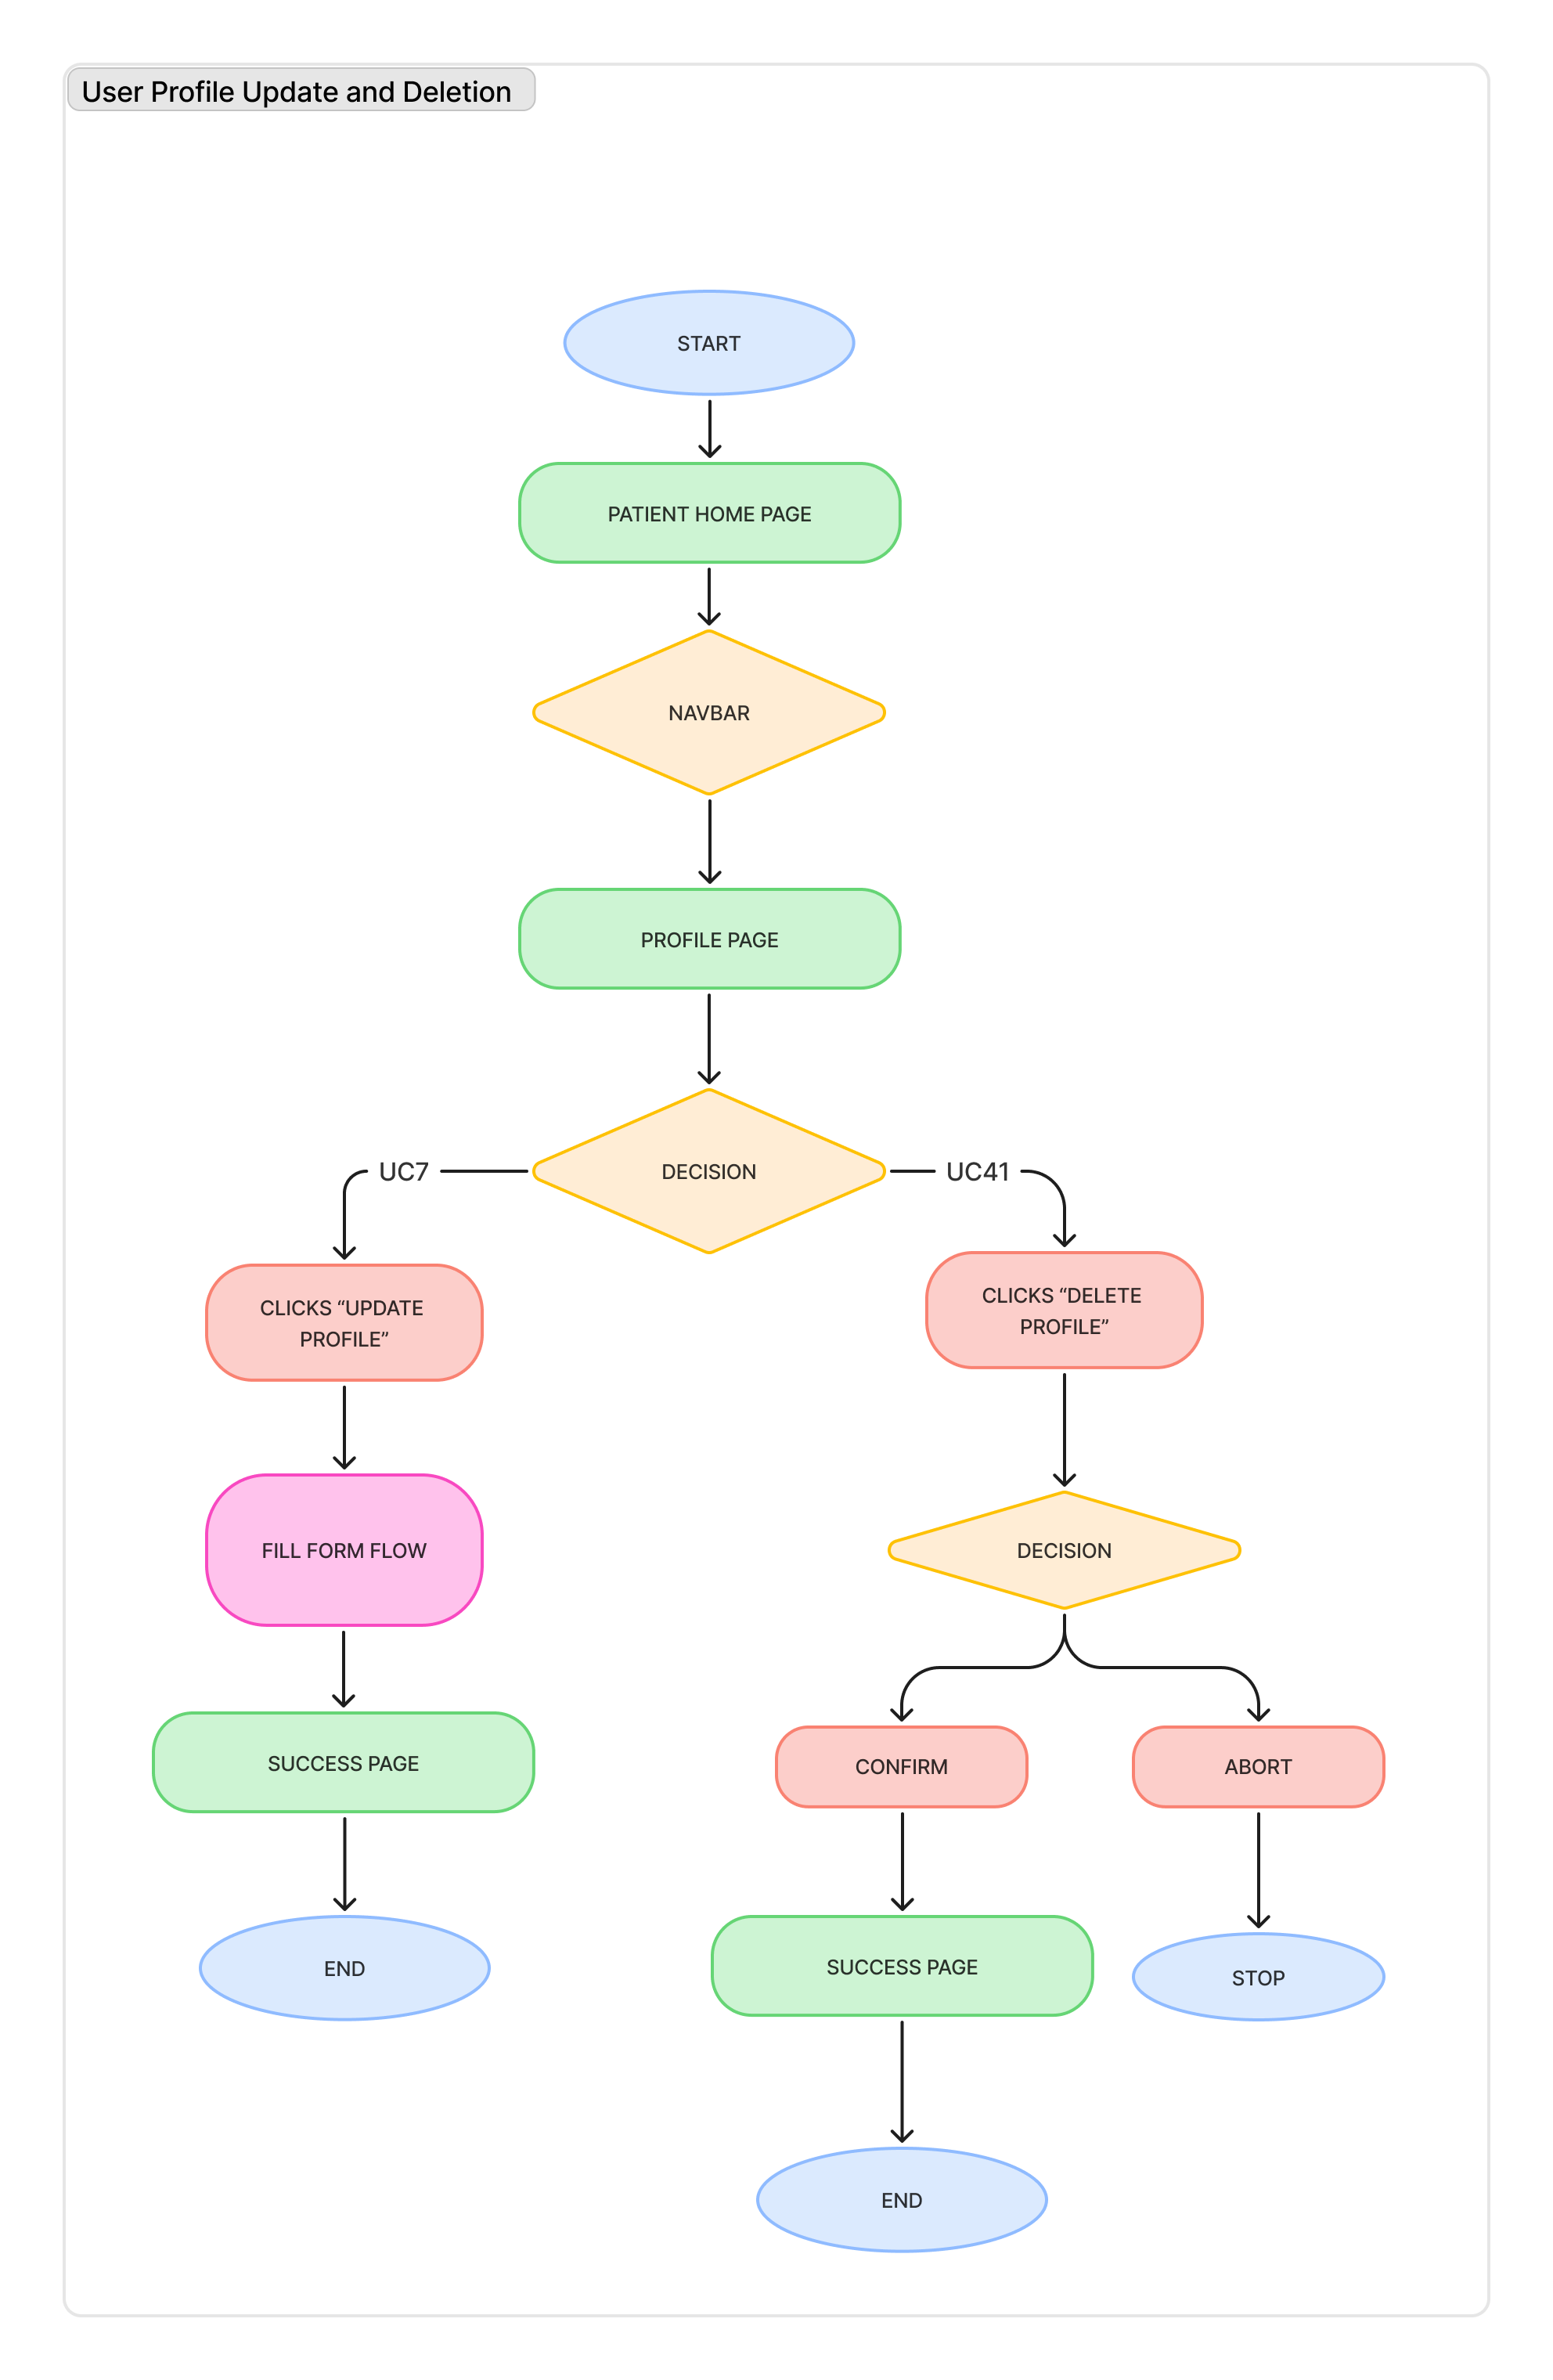
\includegraphics[width=0.8\textwidth]{User_Flows/ProfileUpdateDeletion.png}
        \captionof{figure}{User flow regarding Profile Update and Account Deletion}
    \end{center}
    %\begin{itemize}   
    %\end{itemize}
\end{minipage}
\vspace{3em}

\begin{minipage}{\textwidth}
    \phantomsection
    \subsection{UF4. User - Export Calendar}
    The following user flow shows the steps a user takes to export their appointment to an external calendar.
    It refers to use case \textbf{UC31}, and methods \textbf{??} from the class \textbf{User} of the class diagram.
    
    \begin{center}
        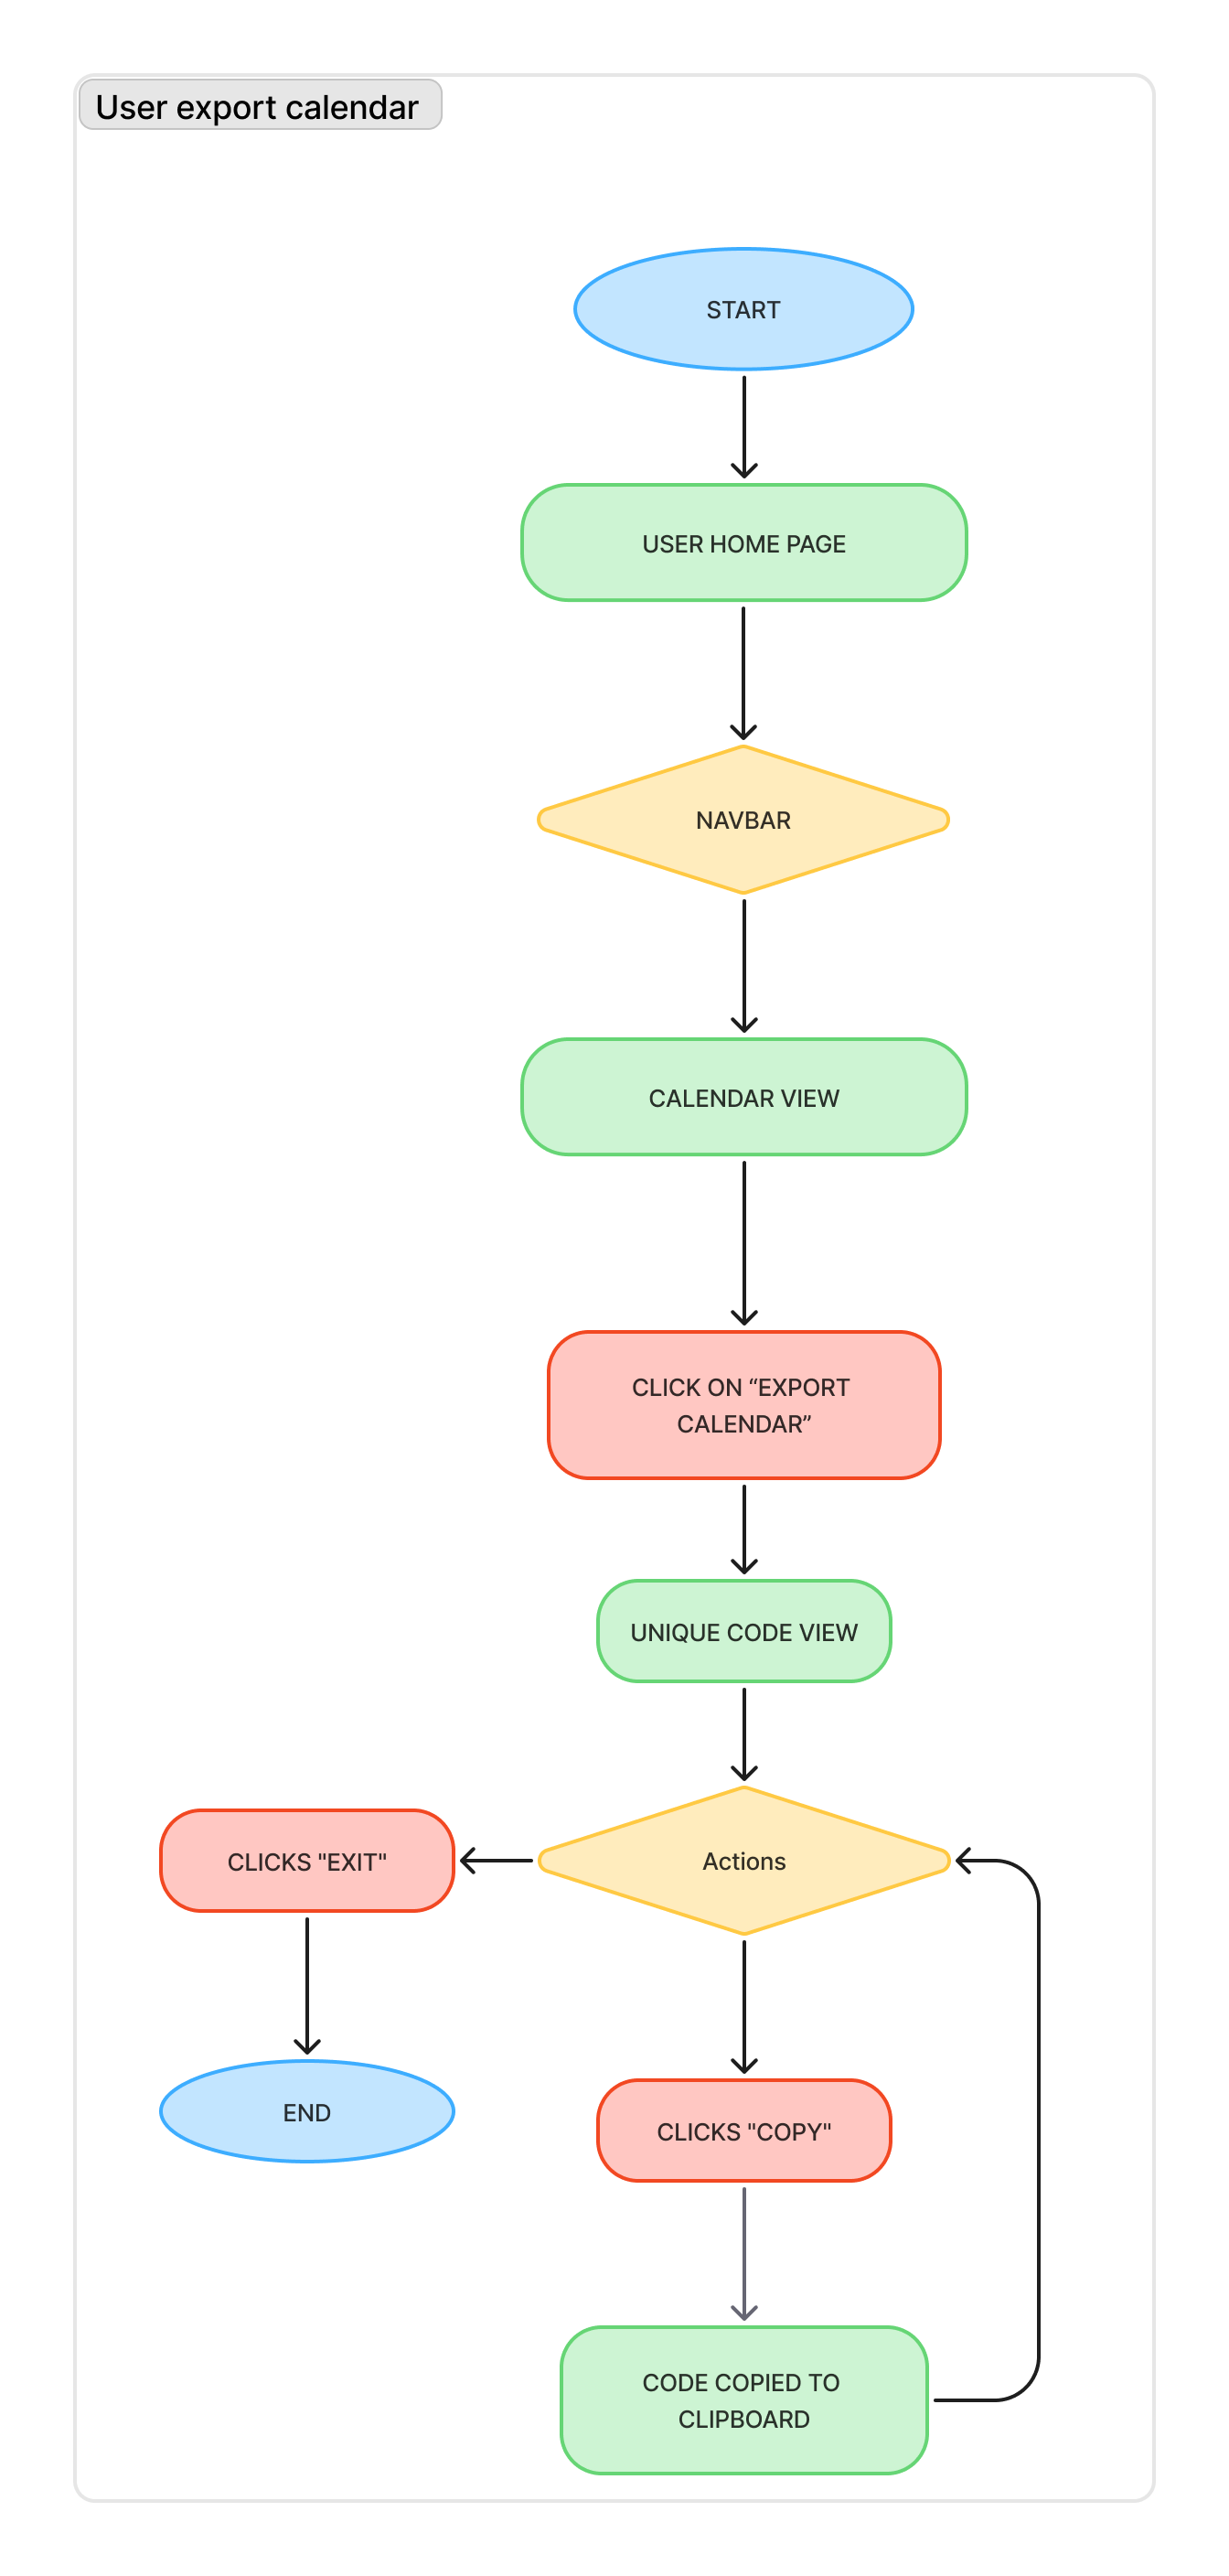
\includegraphics[width=8cm]{User_Flows/ExportCalendar.png}
        \captionof{figure}{User flow regarding Appointment export}
    \end{center}
    %\begin{itemize}   
    %\end{itemize}
\end{minipage}
\vspace{3em}

\begin{minipage}{\textwidth}
    \phantomsection
    \subsection{UF5. Admin - Login}
    The following user flow shows the steps the admin takes to login.
    It refers to use case \textbf{??}, and method \textbf{adminLogin()} from the class \textbf{SystemAdmin} of the class diagram.
    
    \begin{center}
        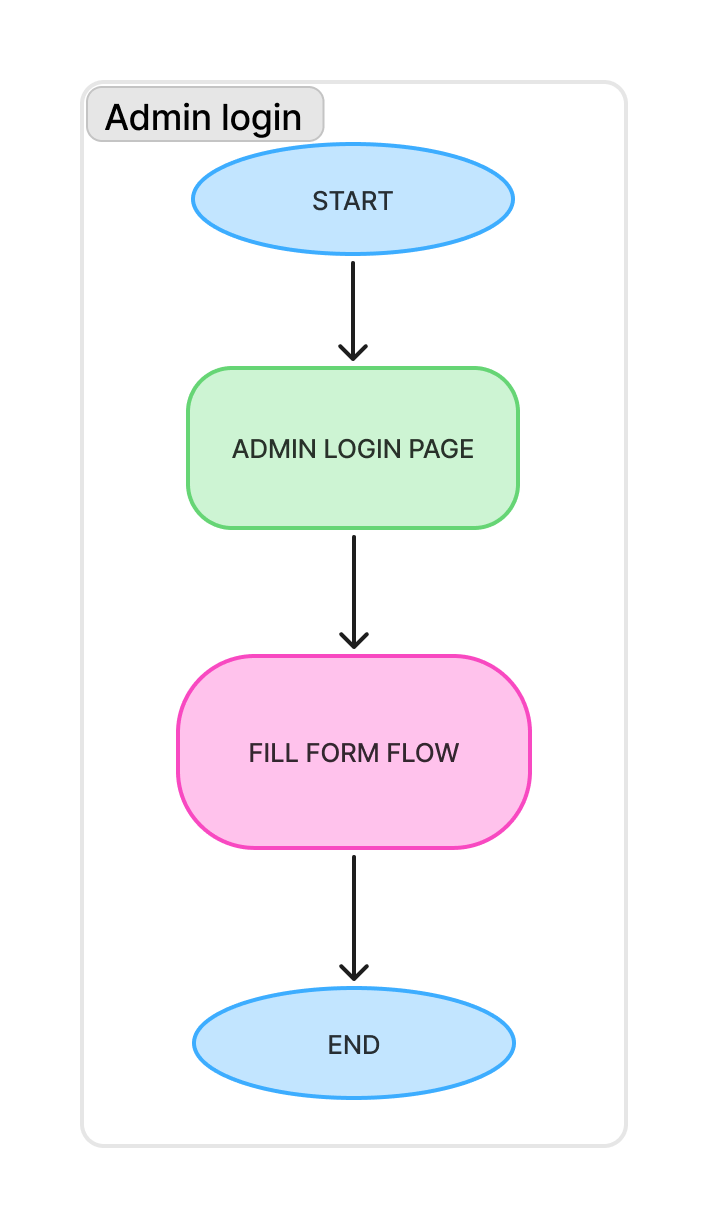
\includegraphics[width=8cm]{User_Flows/AdminLogin.png}
        \captionof{figure}{User flow regarding Admin Login}
    \end{center}
    %\begin{itemize}   
    %\end{itemize}
\end{minipage}
\vspace{3em}

\begin{minipage}{\textwidth}
    \phantomsection
    \subsection{UF6. Admin - Create Insurance Policy, Hospital, Treatment, Department. Register Doctor}
    \label{UF6}
    The following user flow shows the steps the admin takes to create an Insurance Policy, Hospital, Treatment, Department and register a Doctor.
    It refers to use case \textbf{UC1, UC2, UC12}, and methods \textbf{createInsurancePolicy(), createHospital(), createTreatment(), createDepartment(), registerDoctor()} from the class \textbf{SystemAdmin} of the class diagram.
    
    \begin{center}
        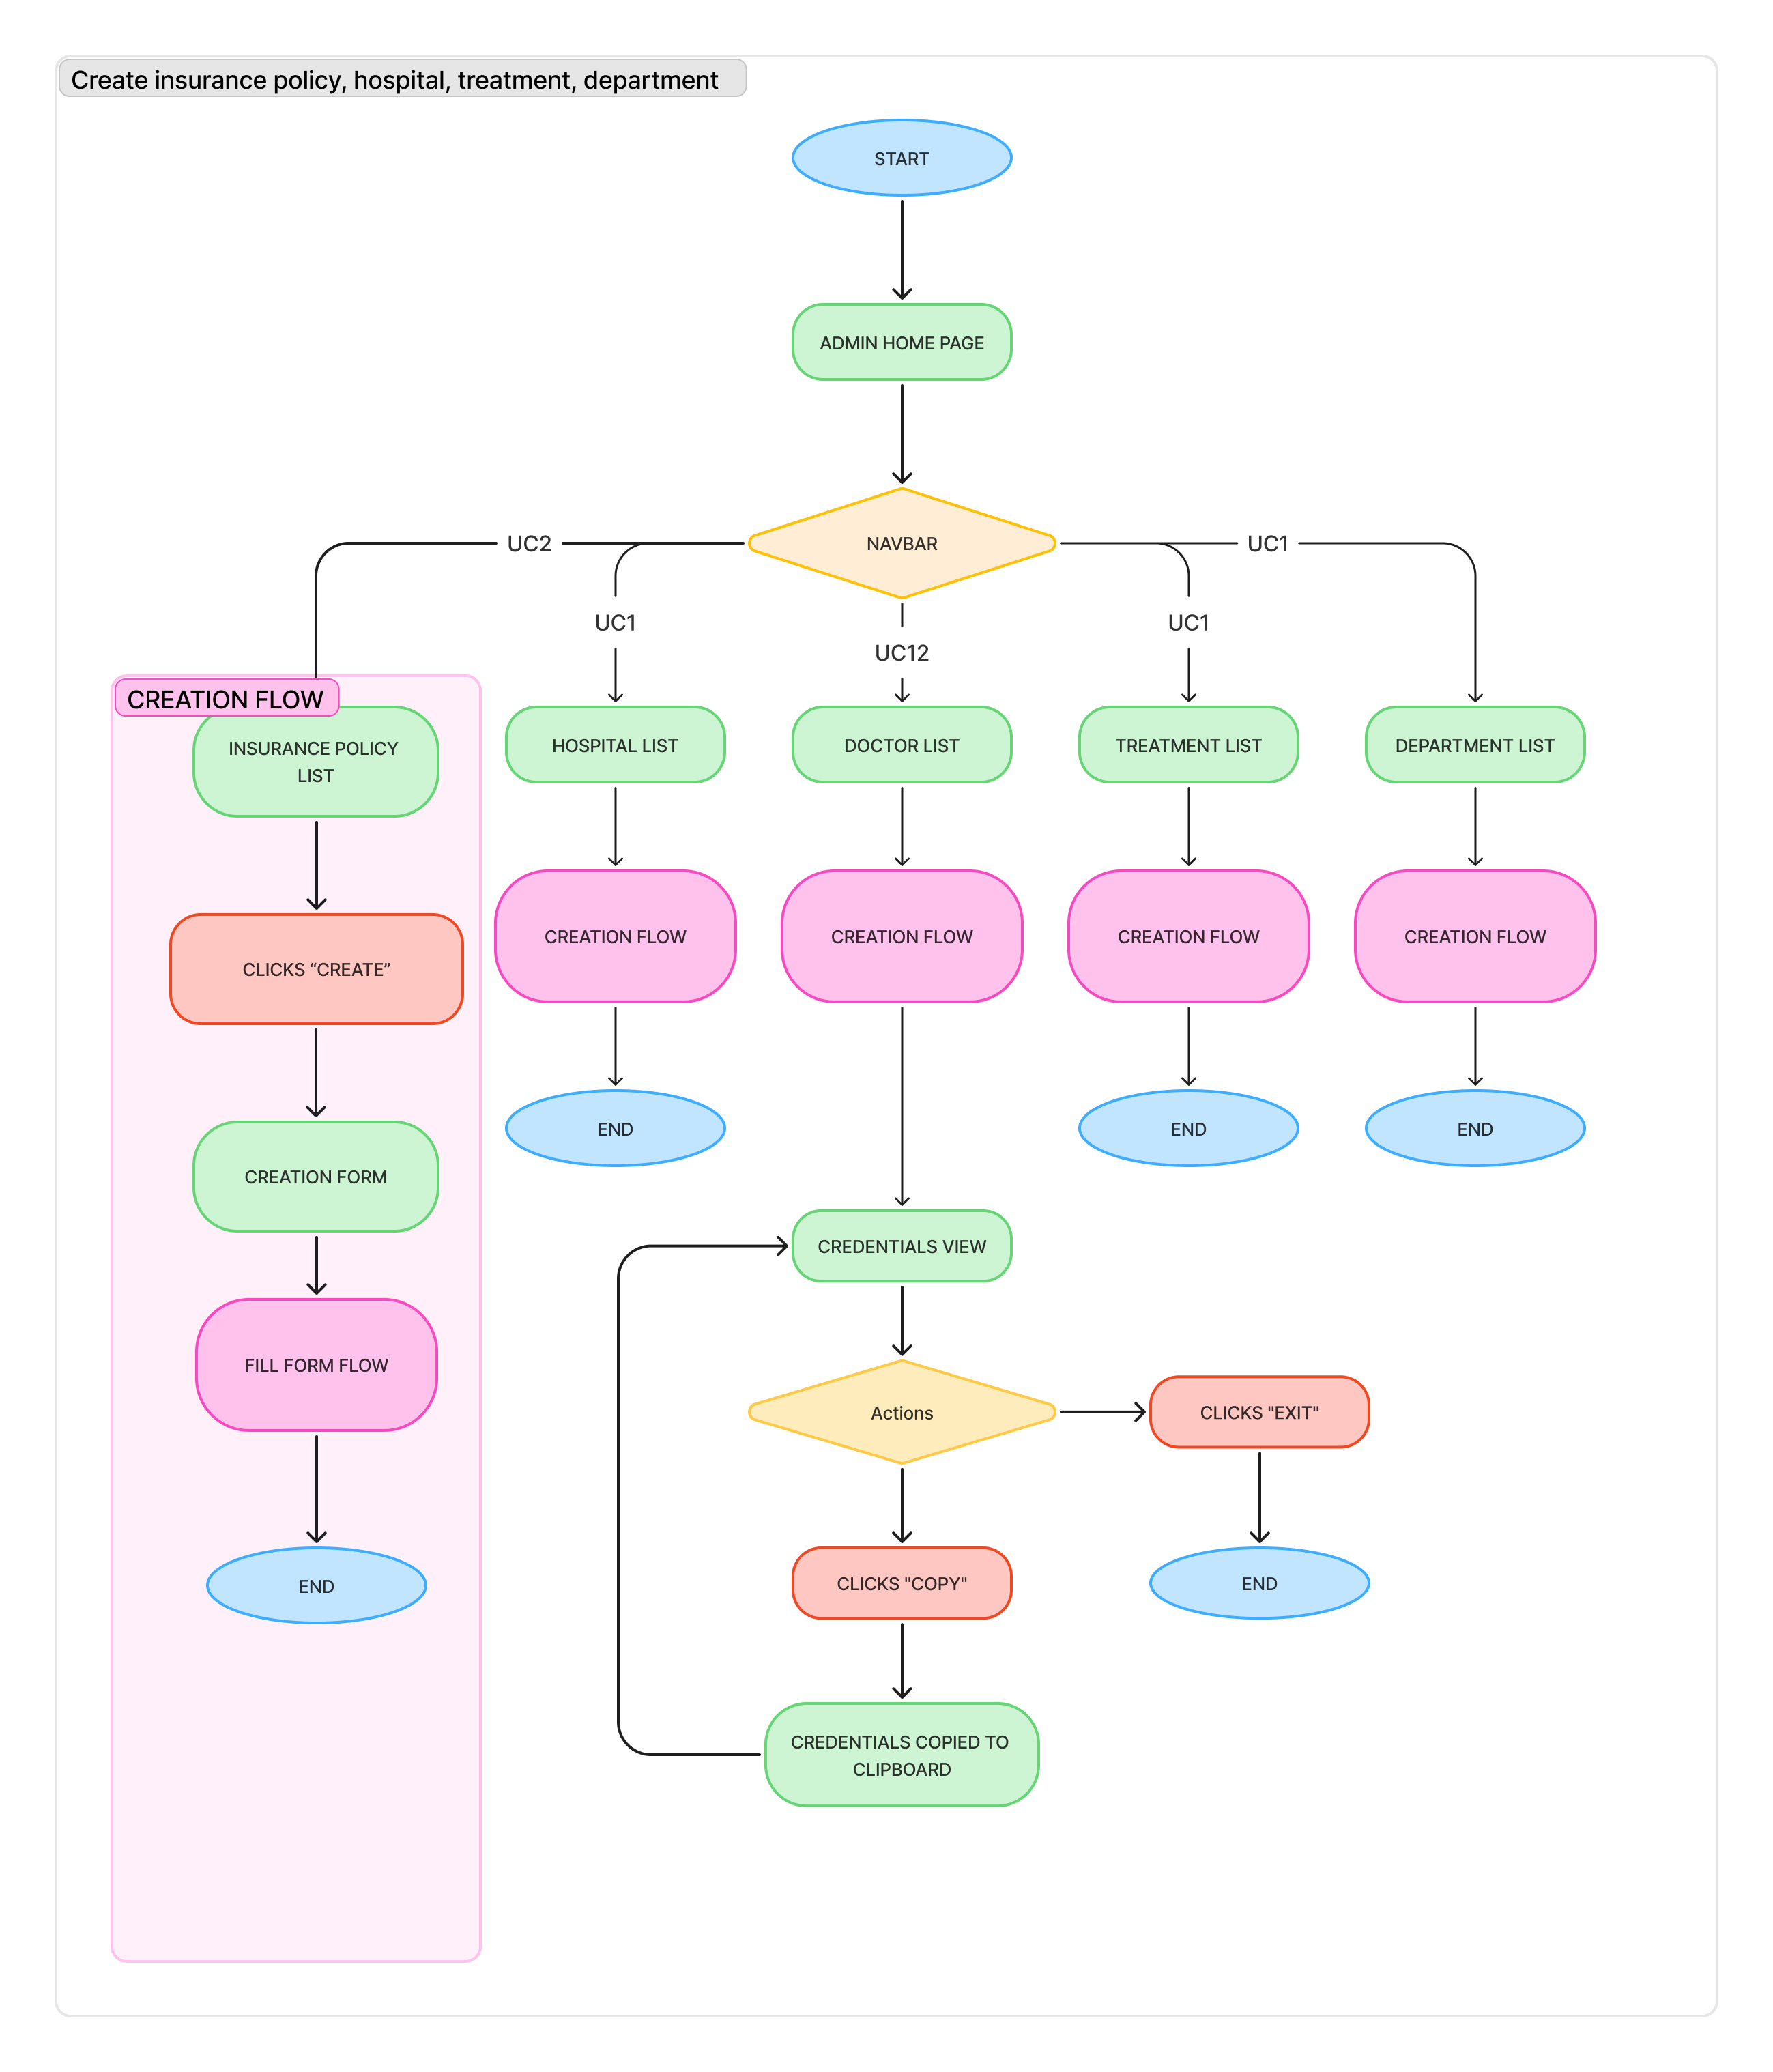
\includegraphics[width=0.8\textwidth]{User_Flows/CreatePolicyHospitalTreatmentDepartment.png}
        \captionof{figure}{User flow regarding Admin Create Insurance Policy, Hospital, Treatment, Department. Register Doctor}
    \end{center}
    %\begin{itemize}   
    %\end{itemize}
\end{minipage}
\vspace{3em}

\begin{minipage}{\textwidth}
    \phantomsection
    \subsection{UF7. Admin - Edit Insurance Policy, Hospital, Treatment, Department}
    \label{UF7}
    The following user flow shows the steps the admin takes to edit an Insurance Policy, Hospital, Treatment, Department.
    It refers to use case \textbf{UC5, UC6}, and methods \textbf{editInsurancePolicy(), editHospital(), editTreatment(), editDepartment()} from the class \textbf{SystemAdmin} of the class diagram.
    
    \begin{center}
        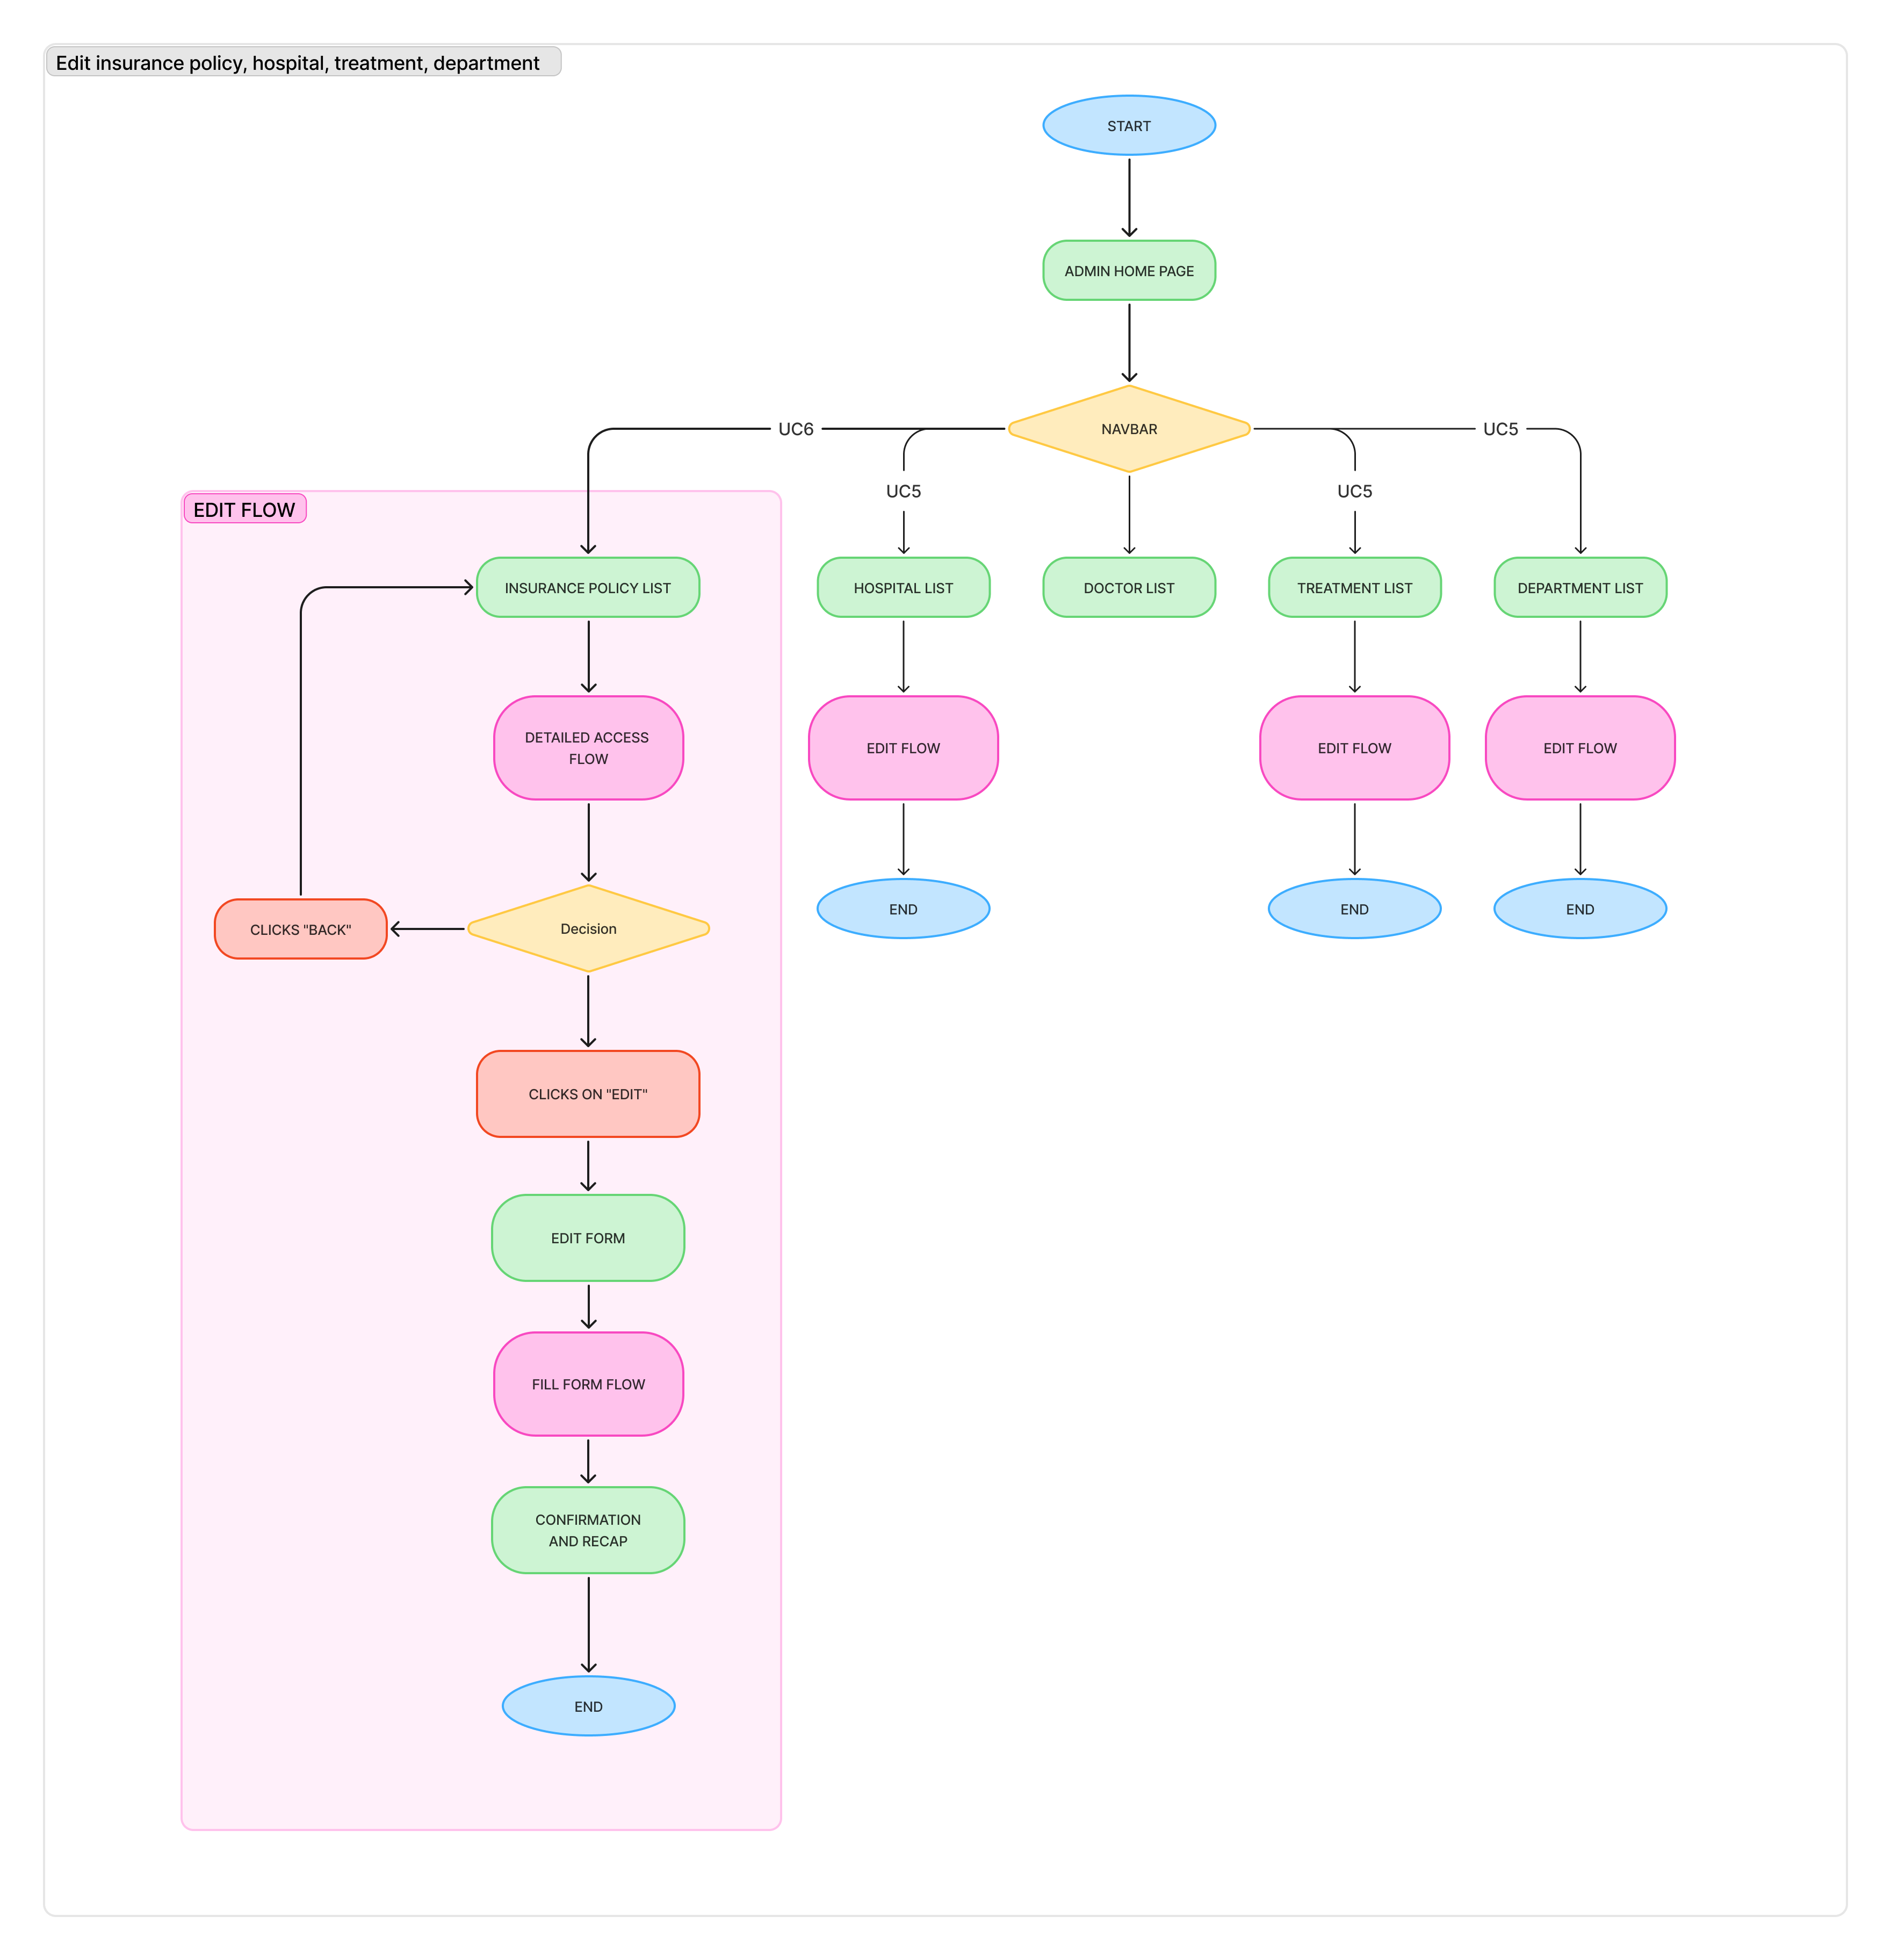
\includegraphics[width=0.8\textwidth]{User_Flows/EditPolicyHospitalTreatmentDepartment.png}
        \captionof{figure}{User flow regarding Edit Insurance Policy, Hospital, Treatment, Department}
    \end{center}
    %\begin{itemize}   
    %\end{itemize}
\end{minipage}
\vspace{3em}

\begin{minipage}{\textwidth}
    \phantomsection
    \subsection{UF8. Admin - Deactivate Insurance Policy, Hospital, Treatment, Department}
    \label{UF8}
    The following user flow shows the steps the admin takes to deactivate an Insurance Policy, Hospital, Treatment, Department.
    It refers to use case \textbf{UC8, UC9}, and methods \textbf{deactivateInsurancePolicy(), closeHospital(), deactivateTreatment(), closeDepartment()} from the class \textbf{SystemAdmin} of the class diagram.
    
    \begin{center}
        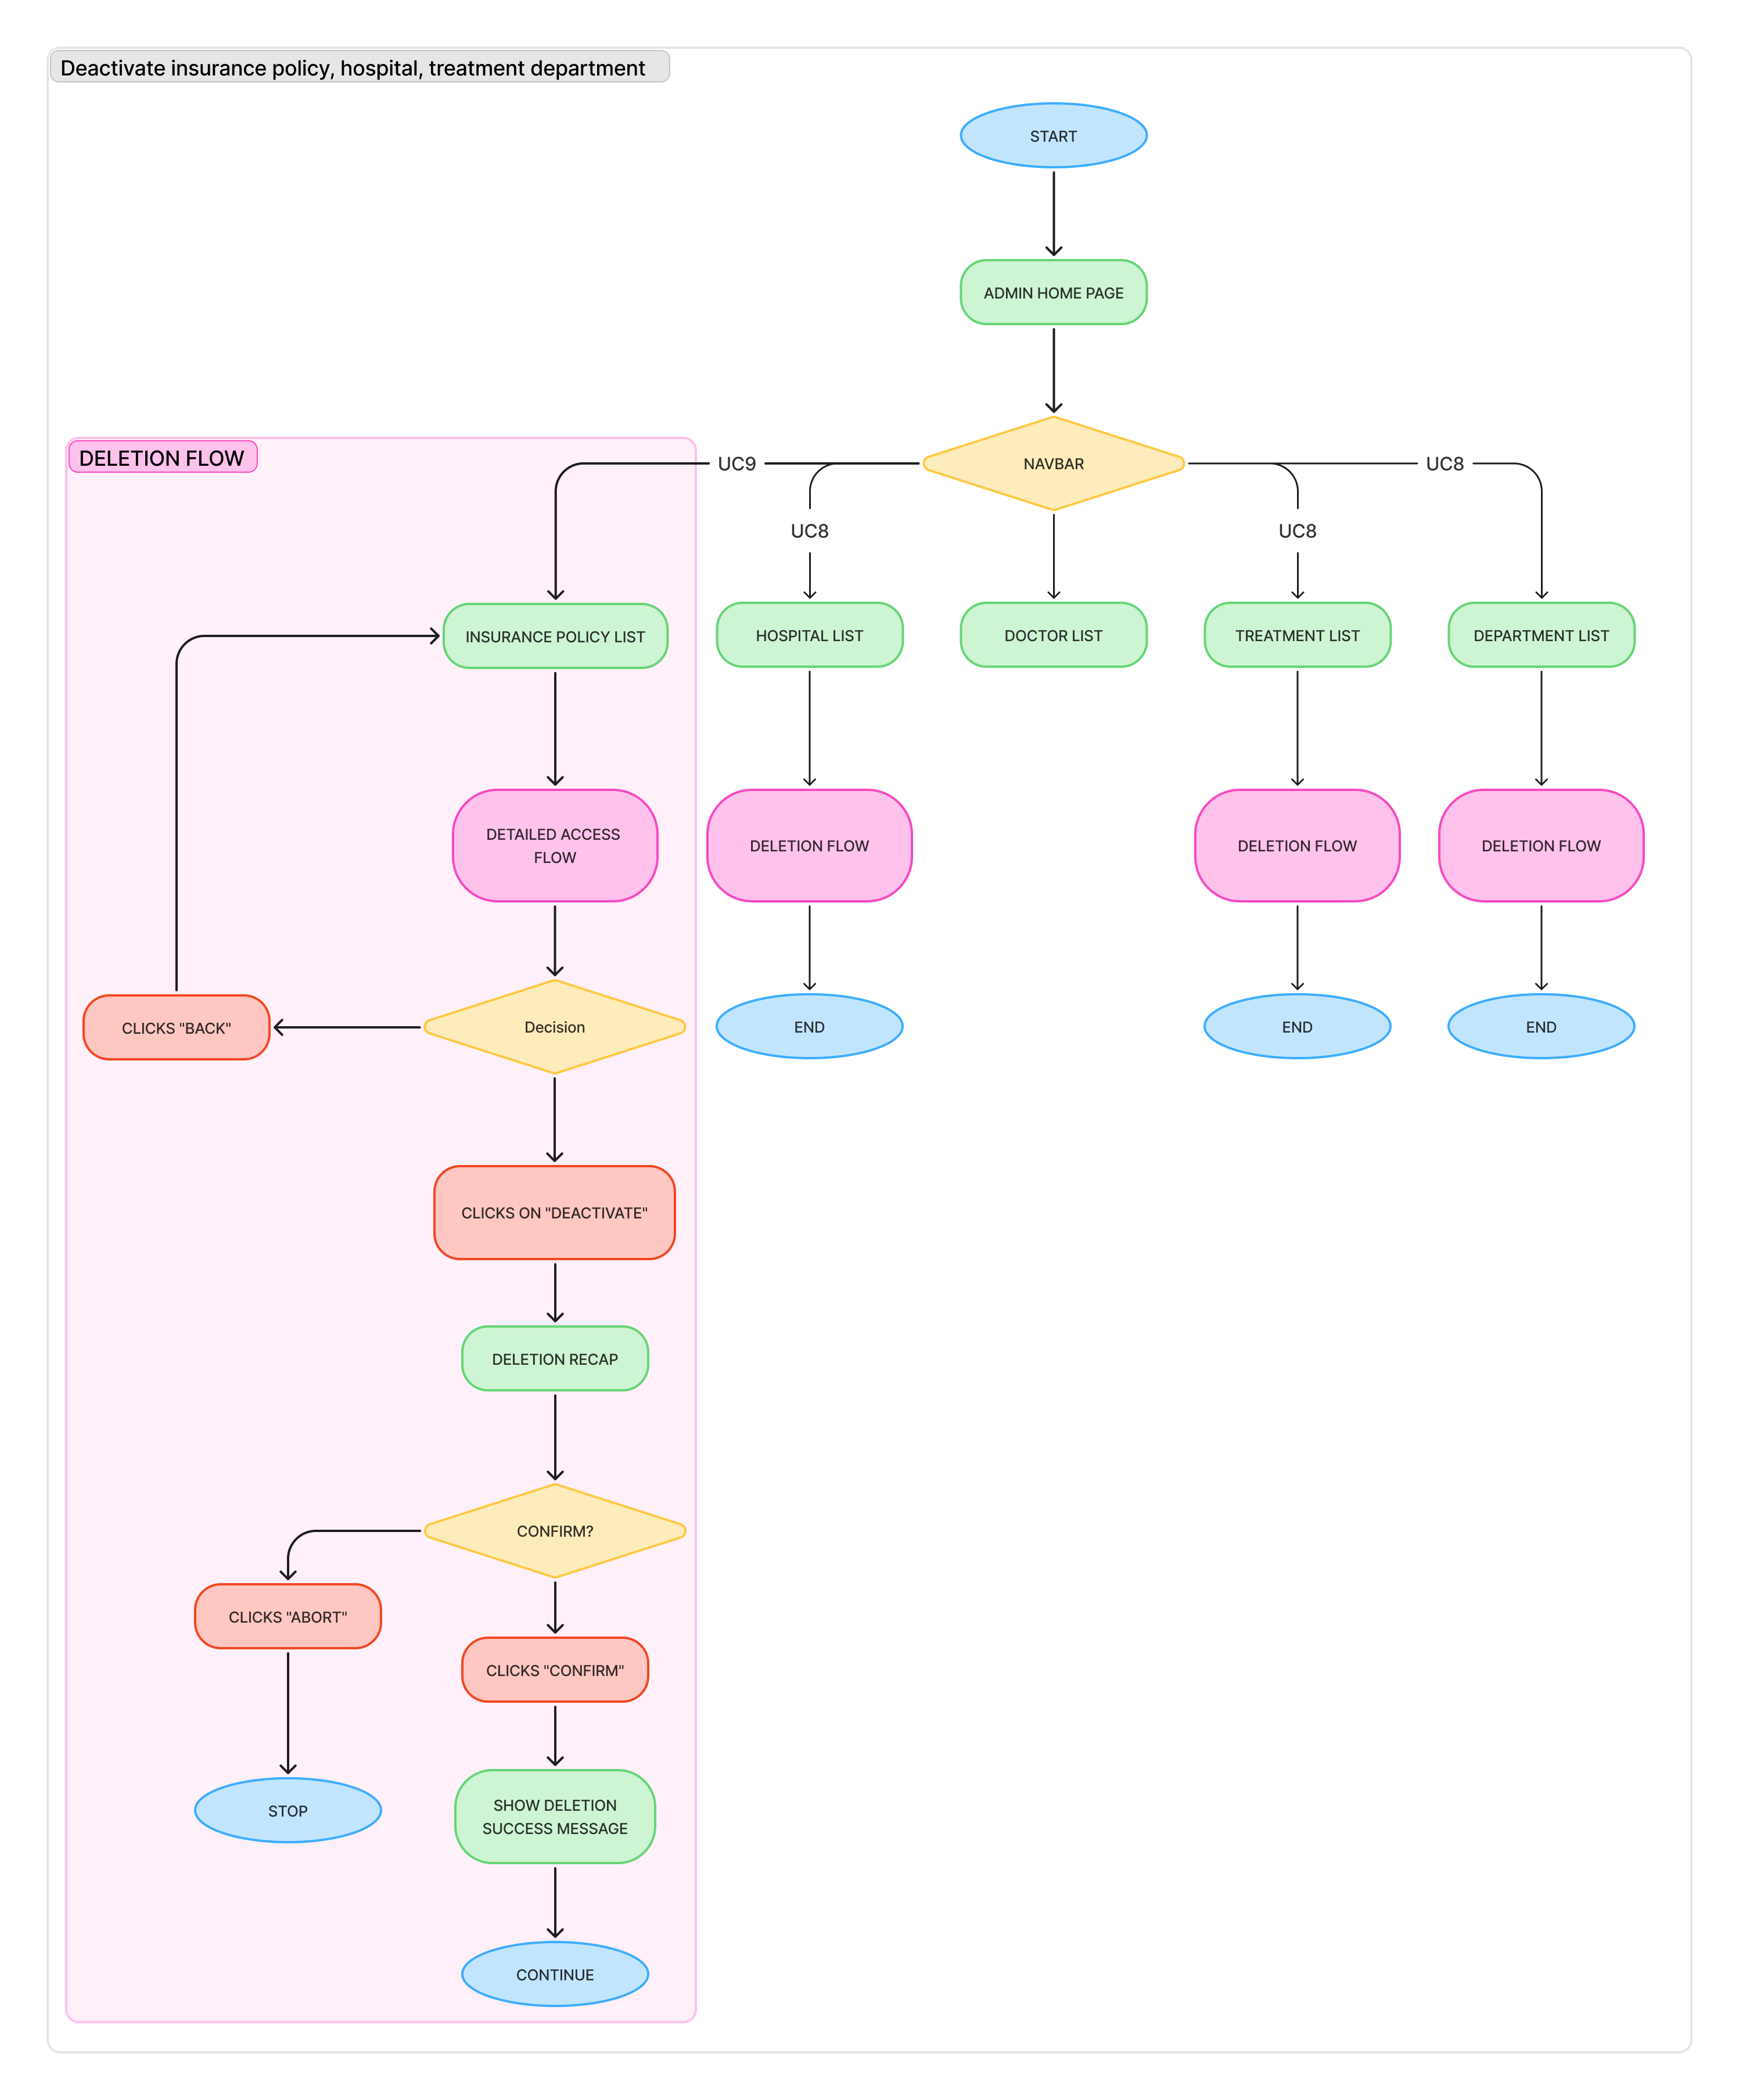
\includegraphics[width=0.8\textwidth]{User_Flows/DeactivatePolicyHospitalTreatmentDepartment.png}
        \captionof{figure}{User flow regarding Deactivate Insurance Policy, Hospital, Treatment, Department}
    \end{center}
    %\begin{itemize}   
    %\end{itemize}
\end{minipage}
\vspace{3em}

\begin{minipage}{\textwidth}
    \phantomsection
    \subsection{UF9. Admin - Appoint Head of Hospital}
    The following user flow shows the steps the admin takes to appoint a Head of Hospital.
    It refers to use case \textbf{UC14}, and methods \textbf{appointHeadOfHospital(doctor:Doctor, hospital: Hospital)} from the class \textbf{SystemAdmin} of the class diagram.
    
    \begin{center}
        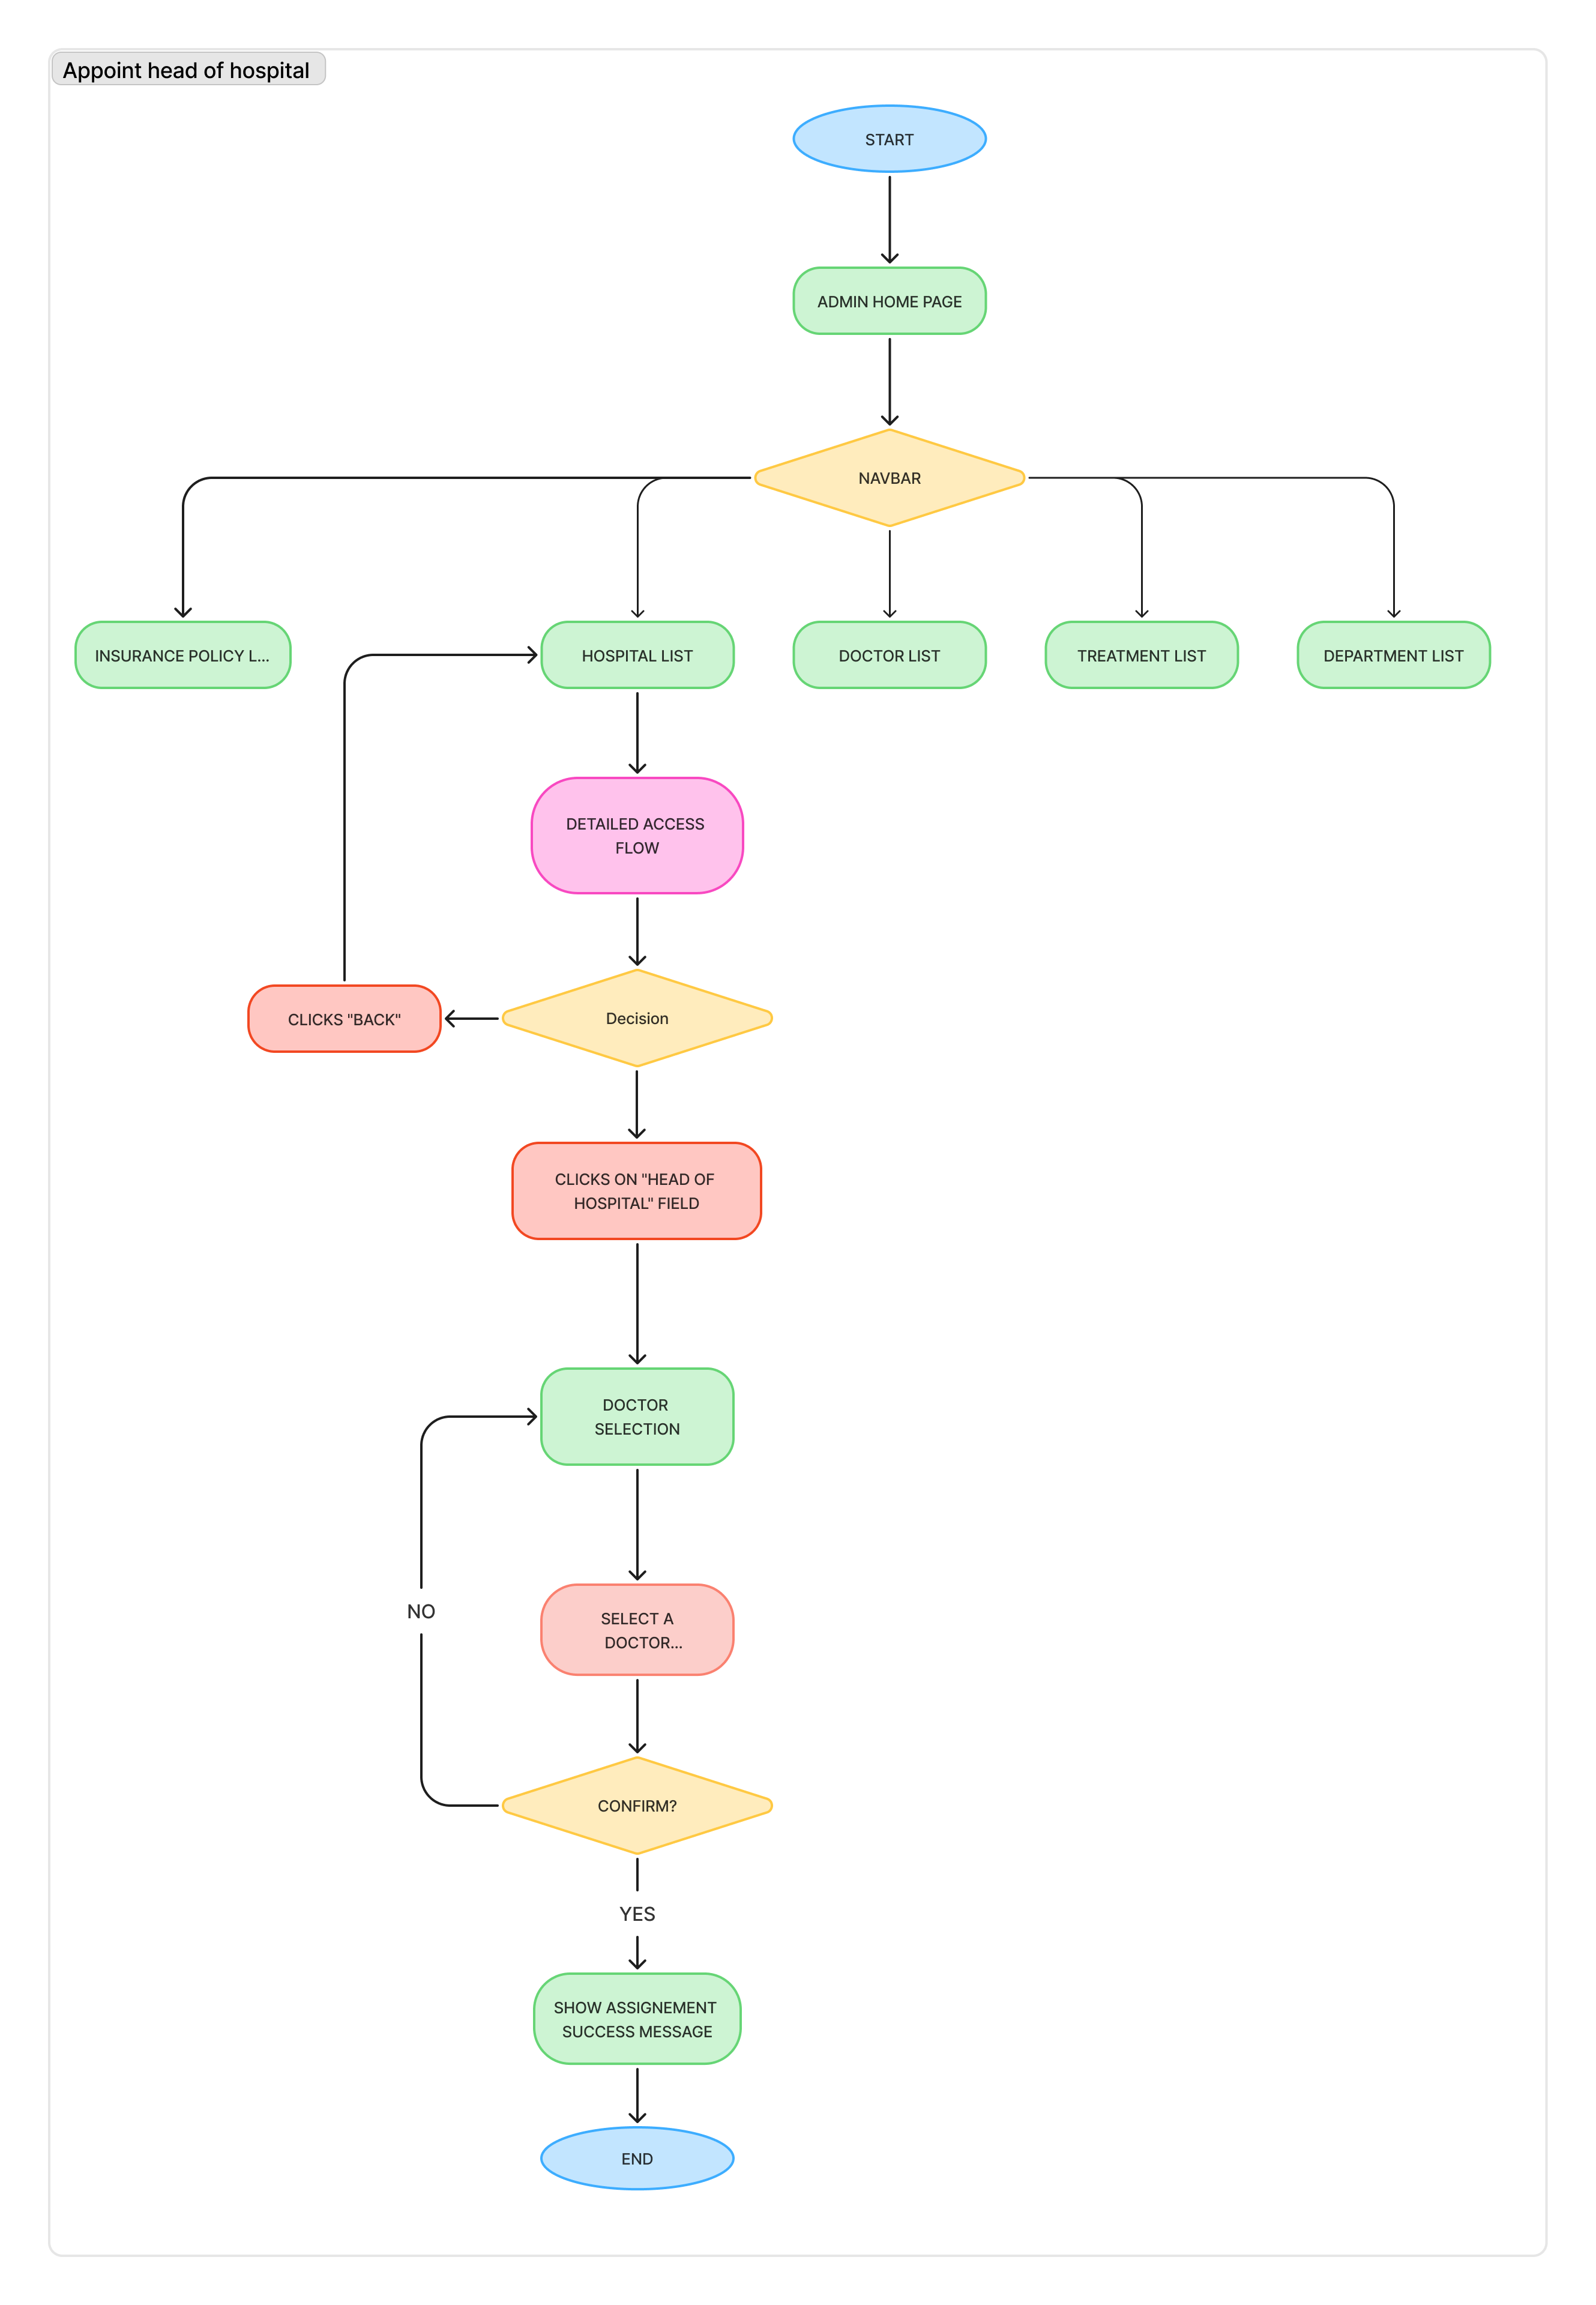
\includegraphics[width=0.8\textwidth]{User_Flows/AppointHeadOfHospital.png}
        \captionof{figure}{User flow regarding Appoint Head of Hospital}
    \end{center}
    %\begin{itemize}   
    %\end{itemize}
\end{minipage}
\vspace{3em}

\begin{minipage}{\textwidth}
    \phantomsection
    \subsection{UF10. Admin - Assign Doctor to Hospital}
    The following user flow shows the steps the admin takes to assign a doctor to a hospital.
    It refers to use case \textbf{UC13}, and methods \textbf{assignDoctorToHospital()} from the class \textbf{SystemAdmin} of the class diagram.
    
    \begin{center}
        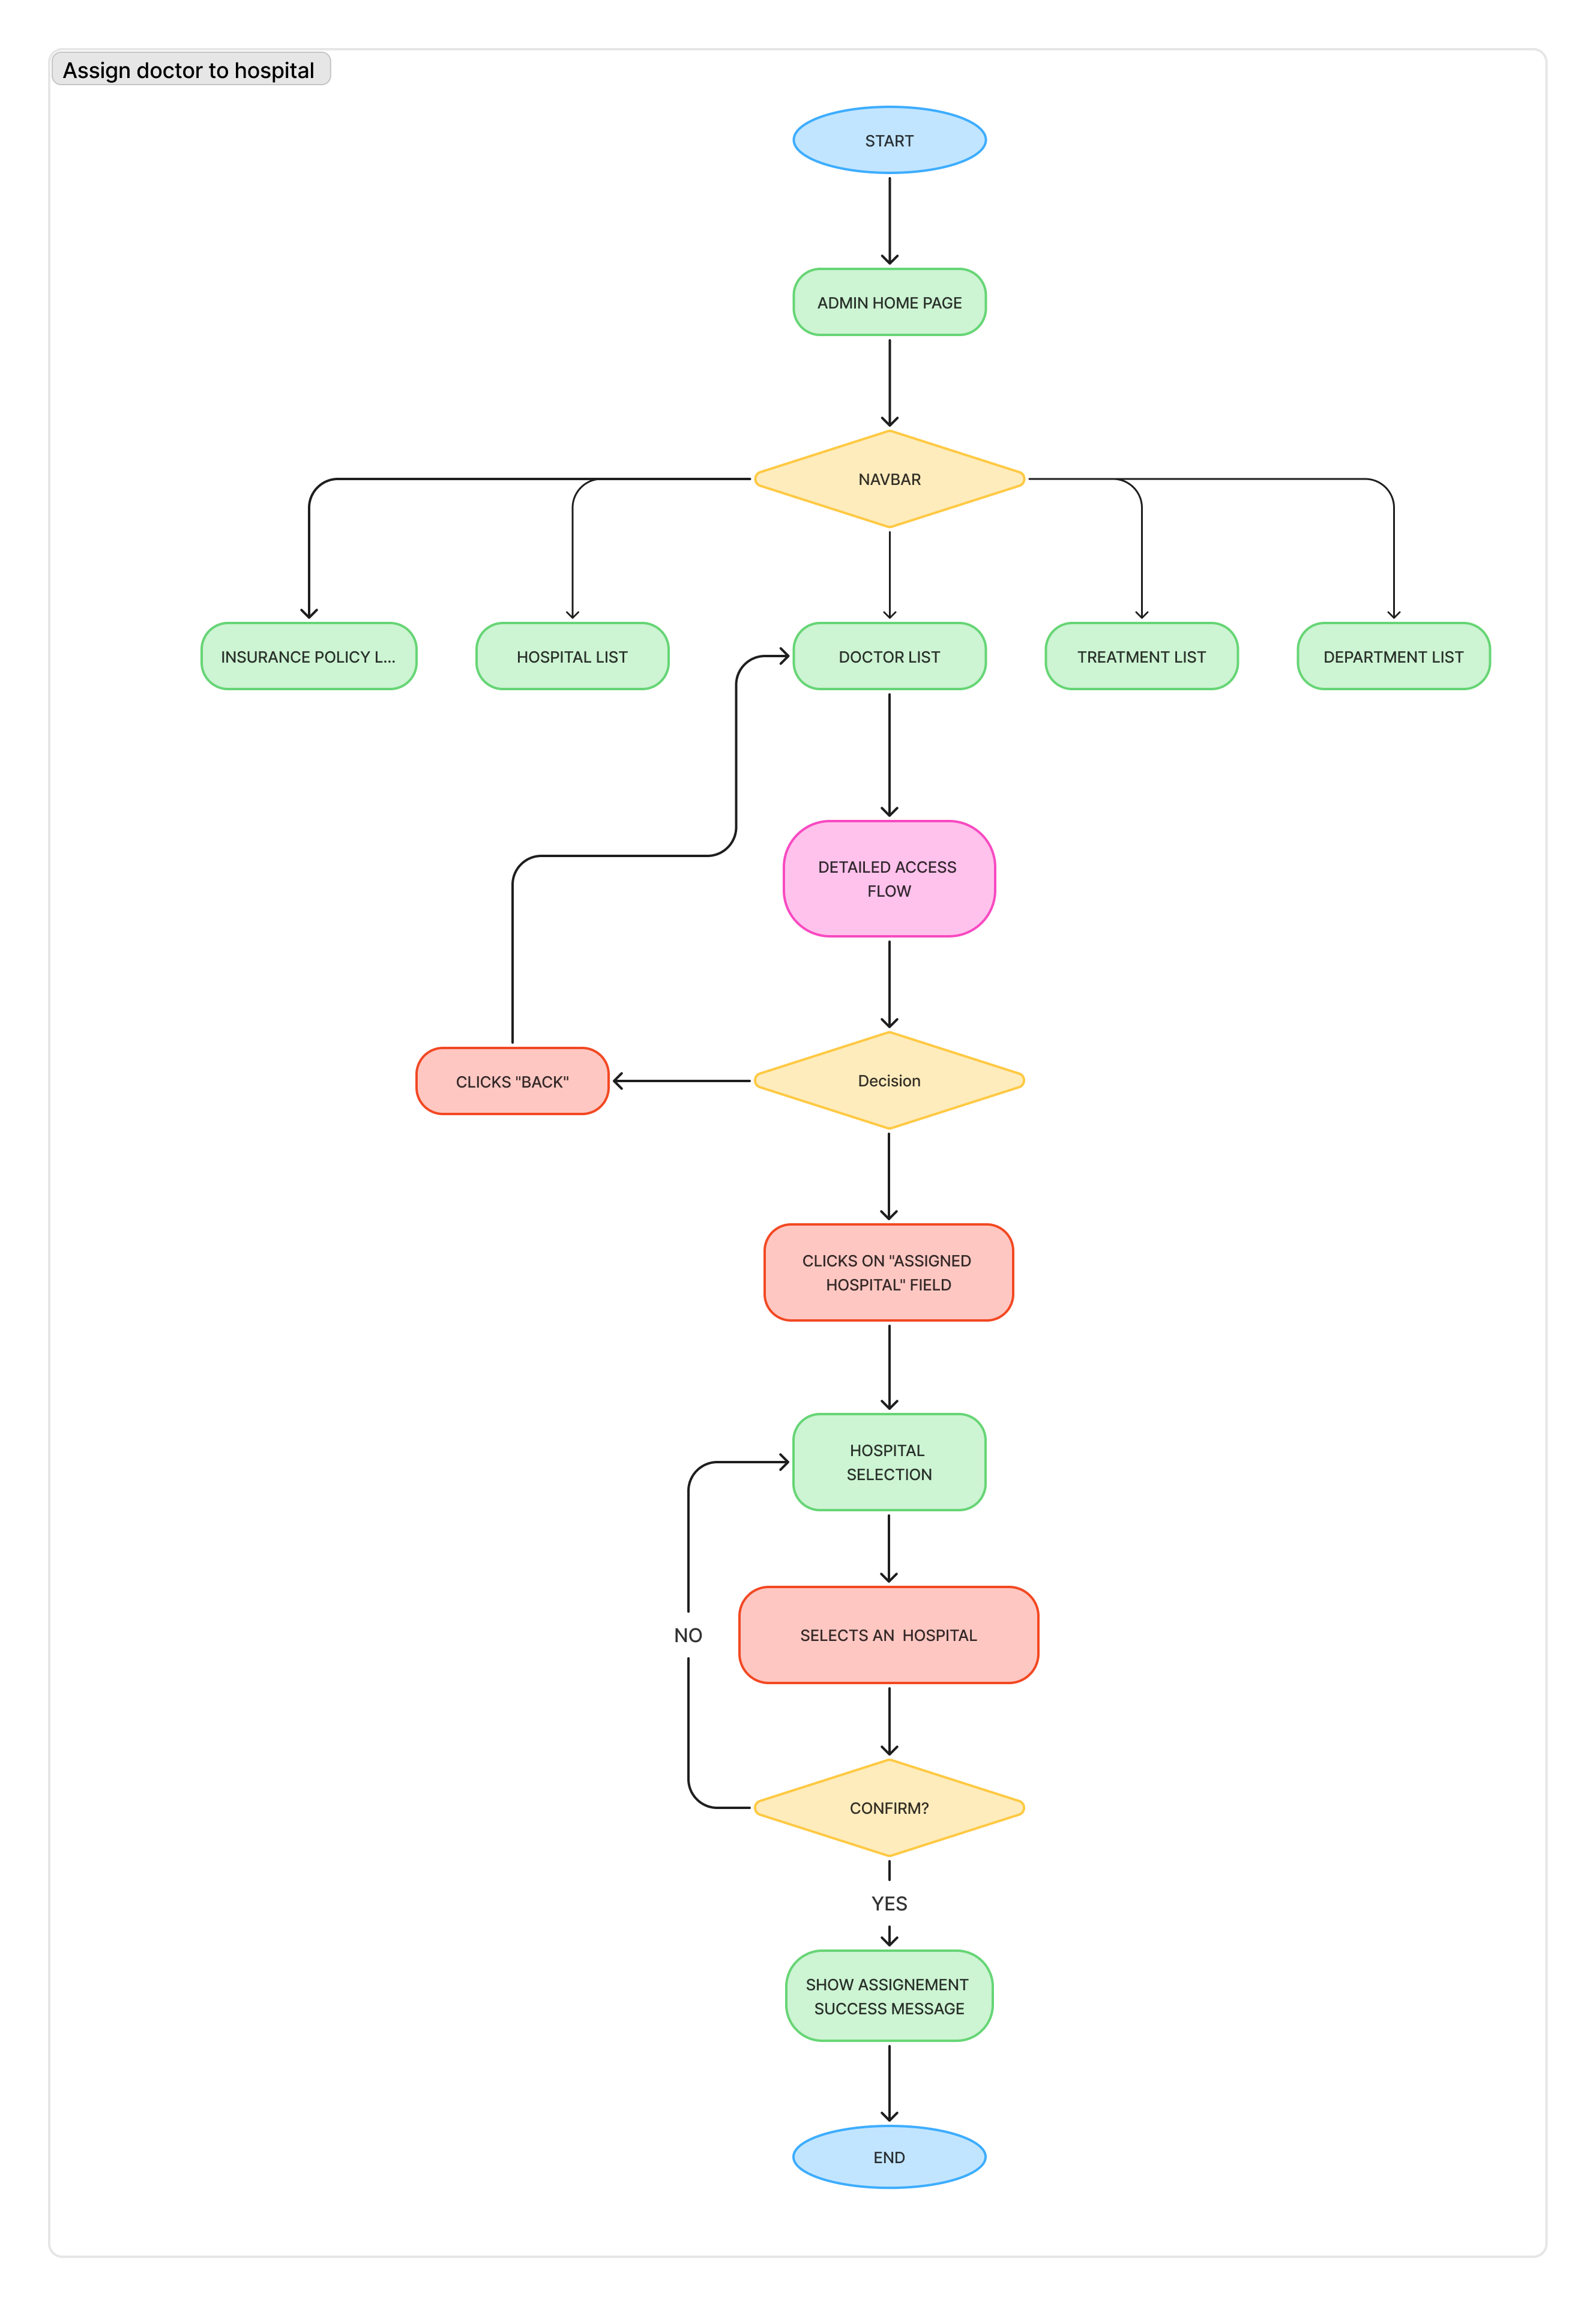
\includegraphics[width=0.8\textwidth]{User_Flows/AssignDoctorHospital.png}
        \captionof{figure}{User flow regarding Assign Doctor to Hospital}
    \end{center}
    %\begin{itemize}   
    %\end{itemize}
\end{minipage}
\vspace{3em}

\begin{minipage}{\textwidth}
    \phantomsection
    \subsection{UF11. Admin - Generate Unique Code}
    The following user flow shows the steps the admin takes to generate a unique insurance policy code.
    It refers to use case \textbf{UC22}, and methods \textbf{generateInsuranceCode(policy:InsurancePolicy, patient:Patient)} from the class \textbf{SystemAdmin} of the class diagram.
    
    \begin{center}
        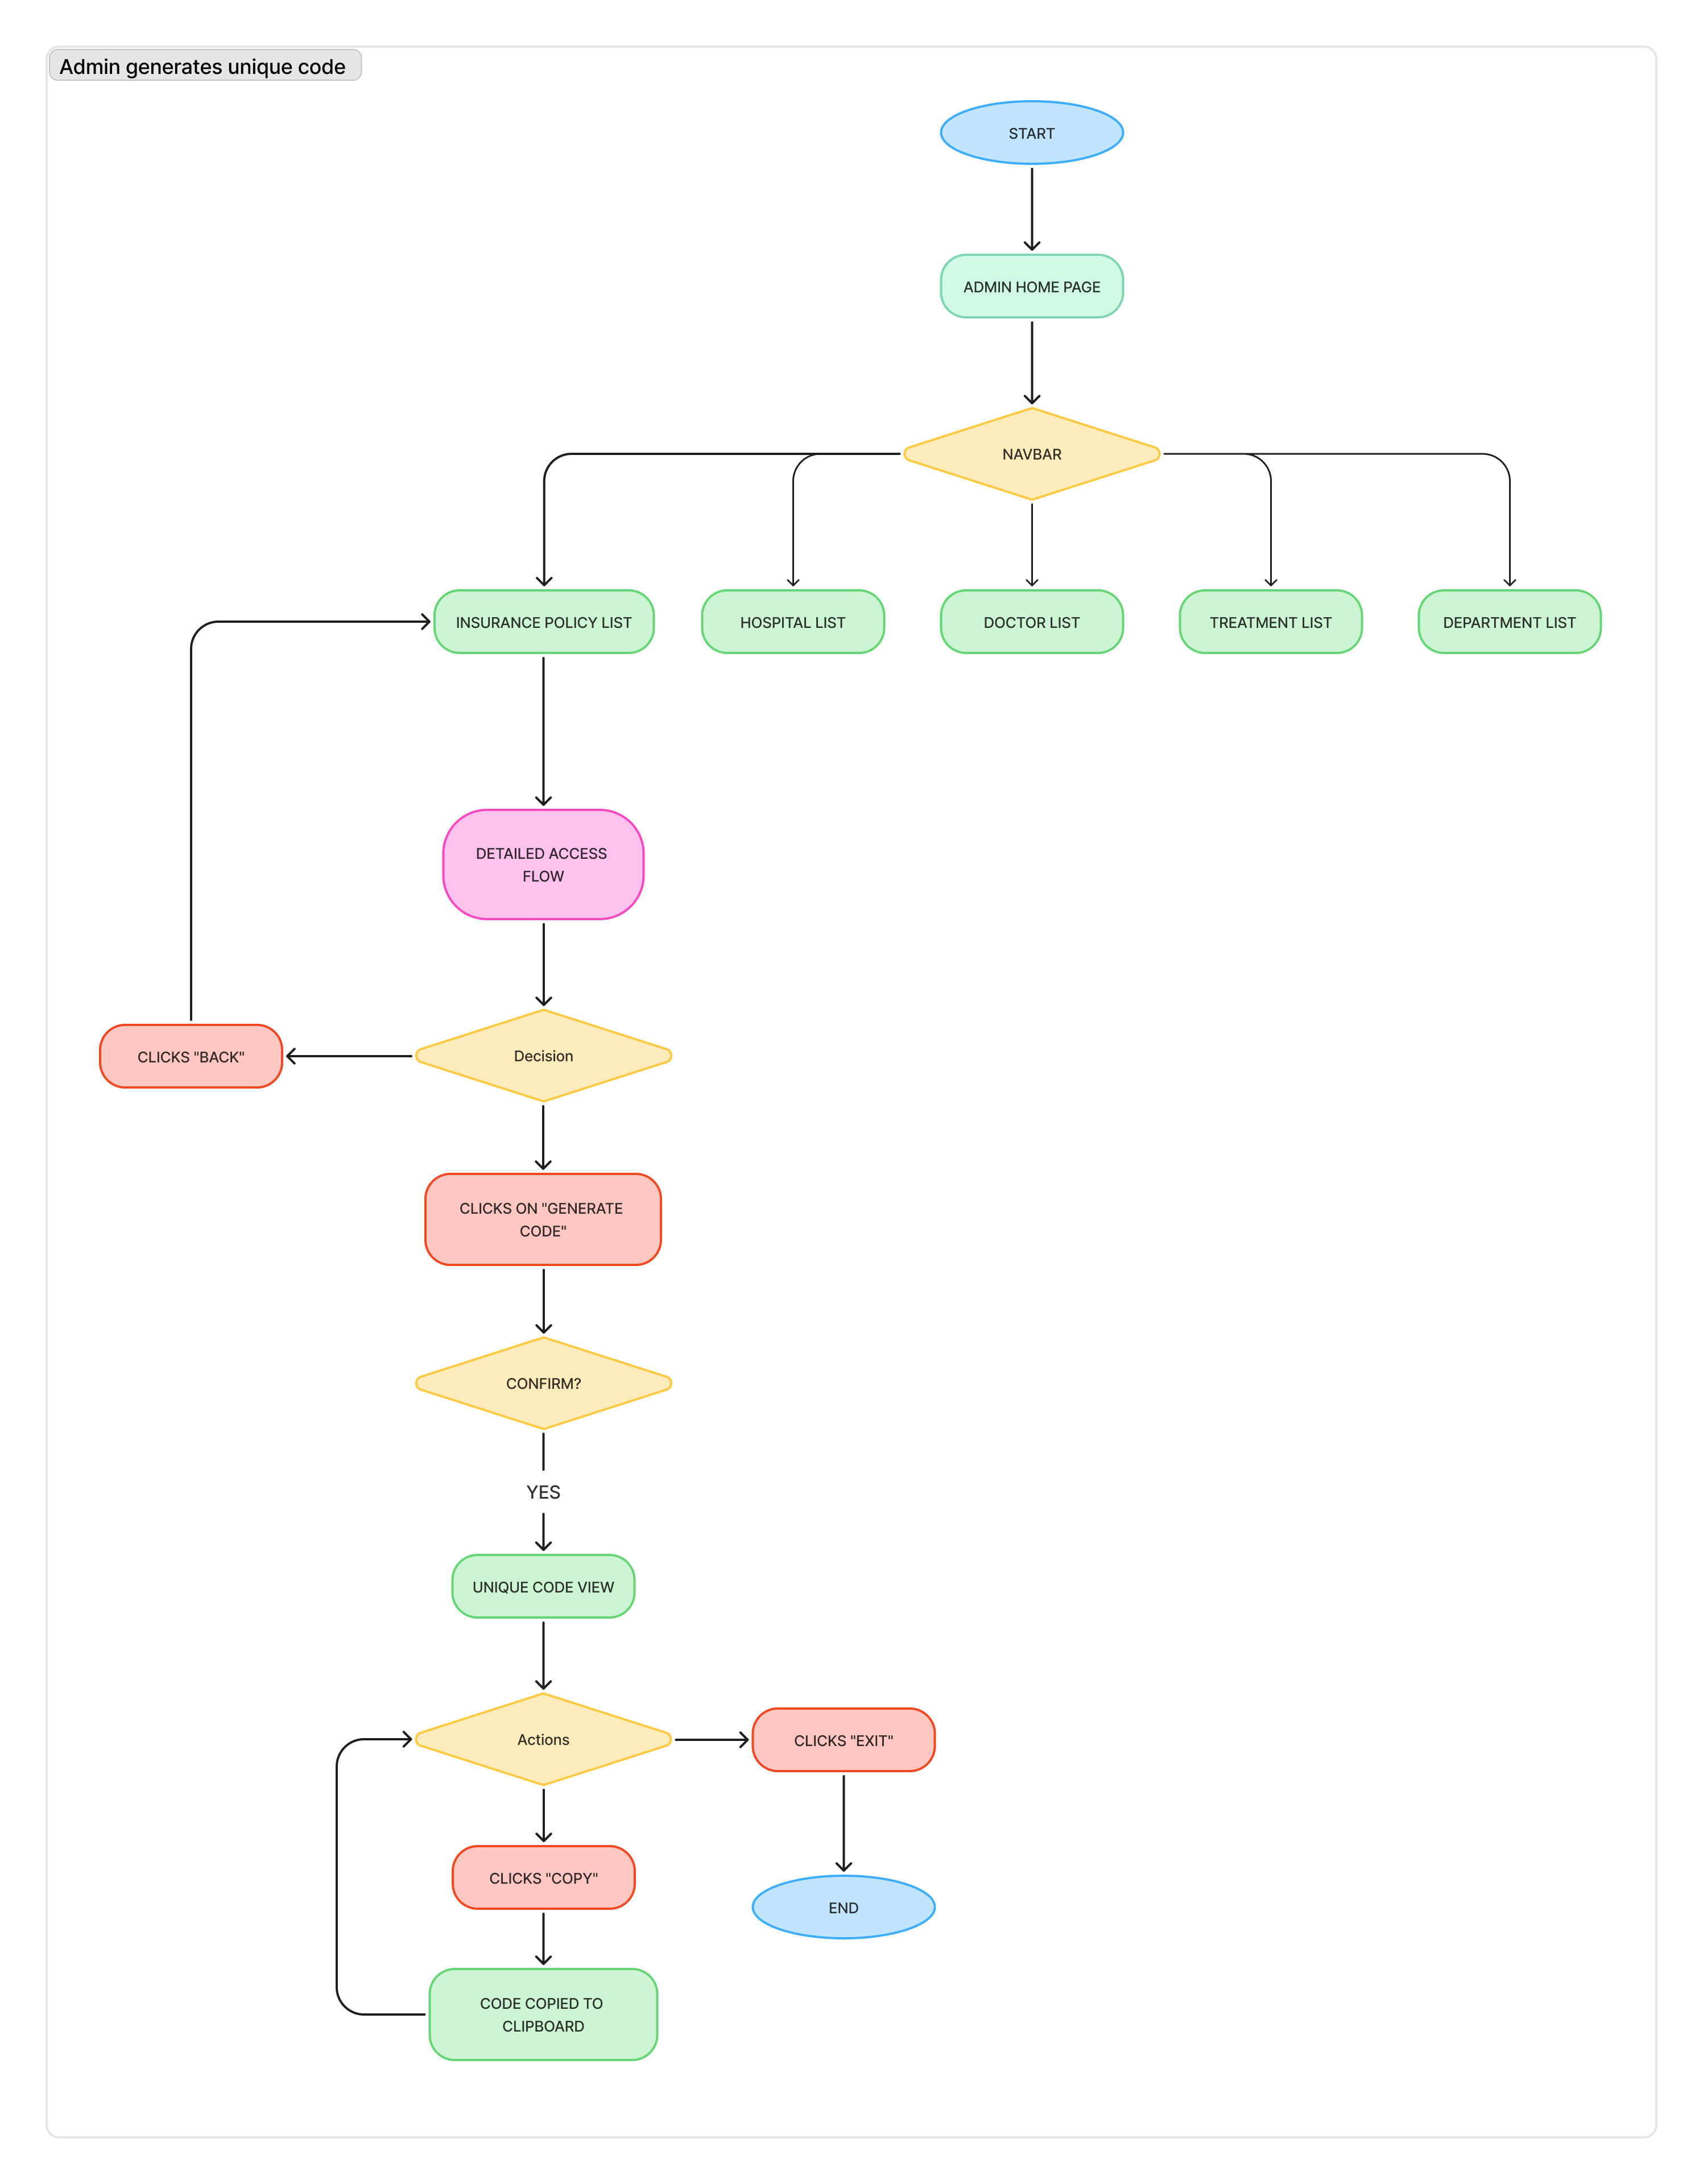
\includegraphics[width=0.8\textwidth]{User_Flows/GenerateUniqueCode.png}
        \captionof{figure}{User flow regarding Generate Unique Code}
    \end{center}
    %\begin{itemize}   
    %\end{itemize}
\end{minipage}
\vspace{3em}

\begin{minipage}{\textwidth}
    \phantomsection
    \subsection{UF12. Patient - Registration and Validation}
    \label{UF12}
    The following user flow shows the process of Patient registration and validation.
    It refers to use case \textbf{UC23}, and methods \textbf{??, ??} from the class \textbf{Patient} of the class diagram.
    
    \begin{center}
        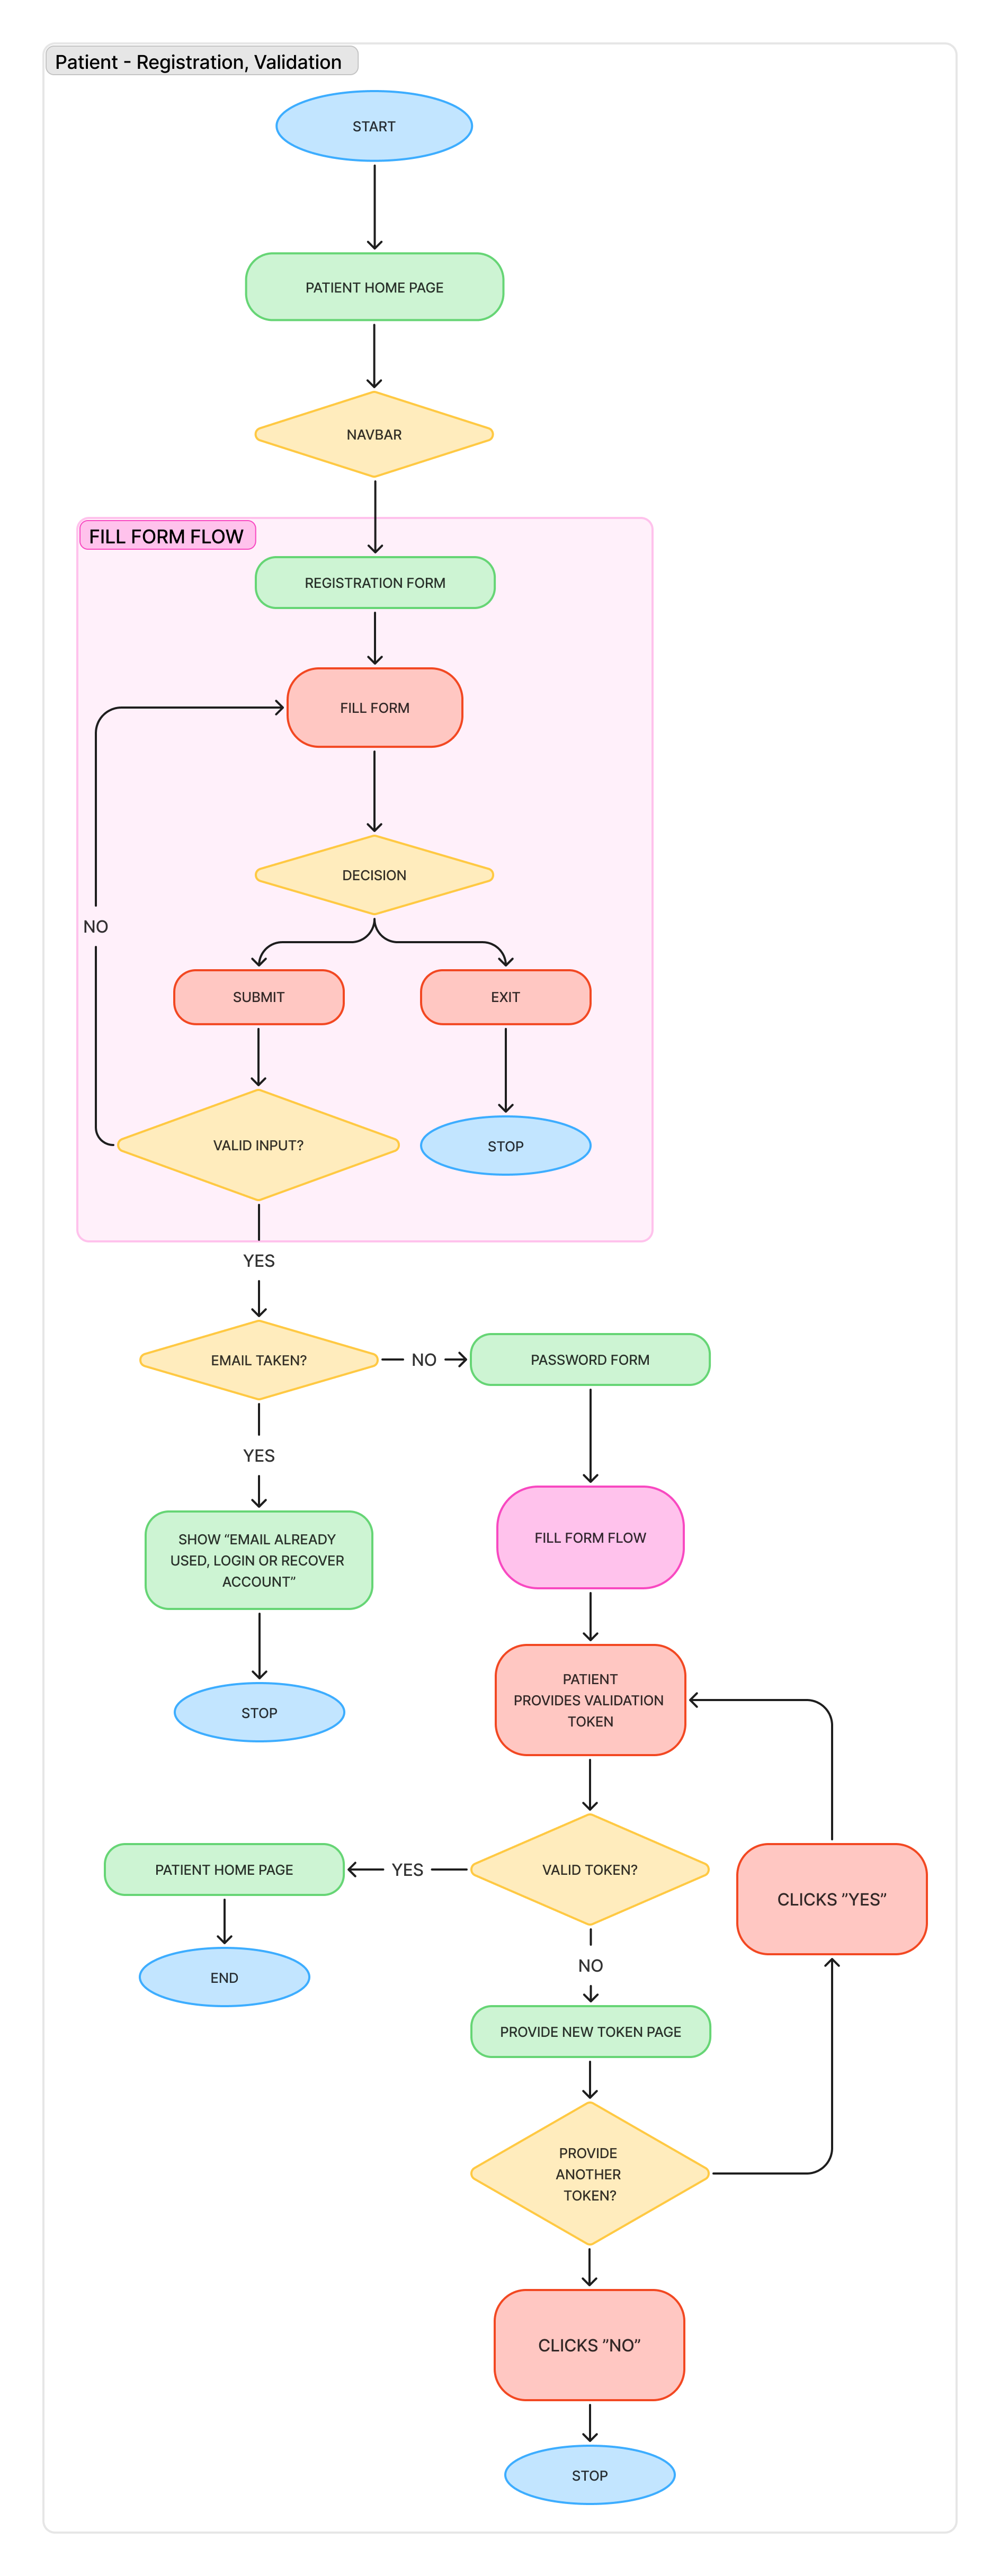
\includegraphics[width=8cm]{User_Flows/PatientRegistrationValidation.png}
        \captionof{figure}{User flow regarding Patient Registration and Validation}
    \end{center}
    %\begin{itemize}   
    %\end{itemize}
\end{minipage}
\vspace{3em}

\begin{minipage}{\textwidth}
    \phantomsection
    \subsection{UF13. Patient - Appointment Cancellation and Rescheduling}
    The following user flow shows the steps a patient takes to cancel and reschedule an appointment.
    It refers to use case \textbf{UC10, UC29}, and methods \textbf{cancelAppointment(), rescheduleAppointment()} from the class \textbf{Patient} of the class diagram.
    
    \begin{center}
        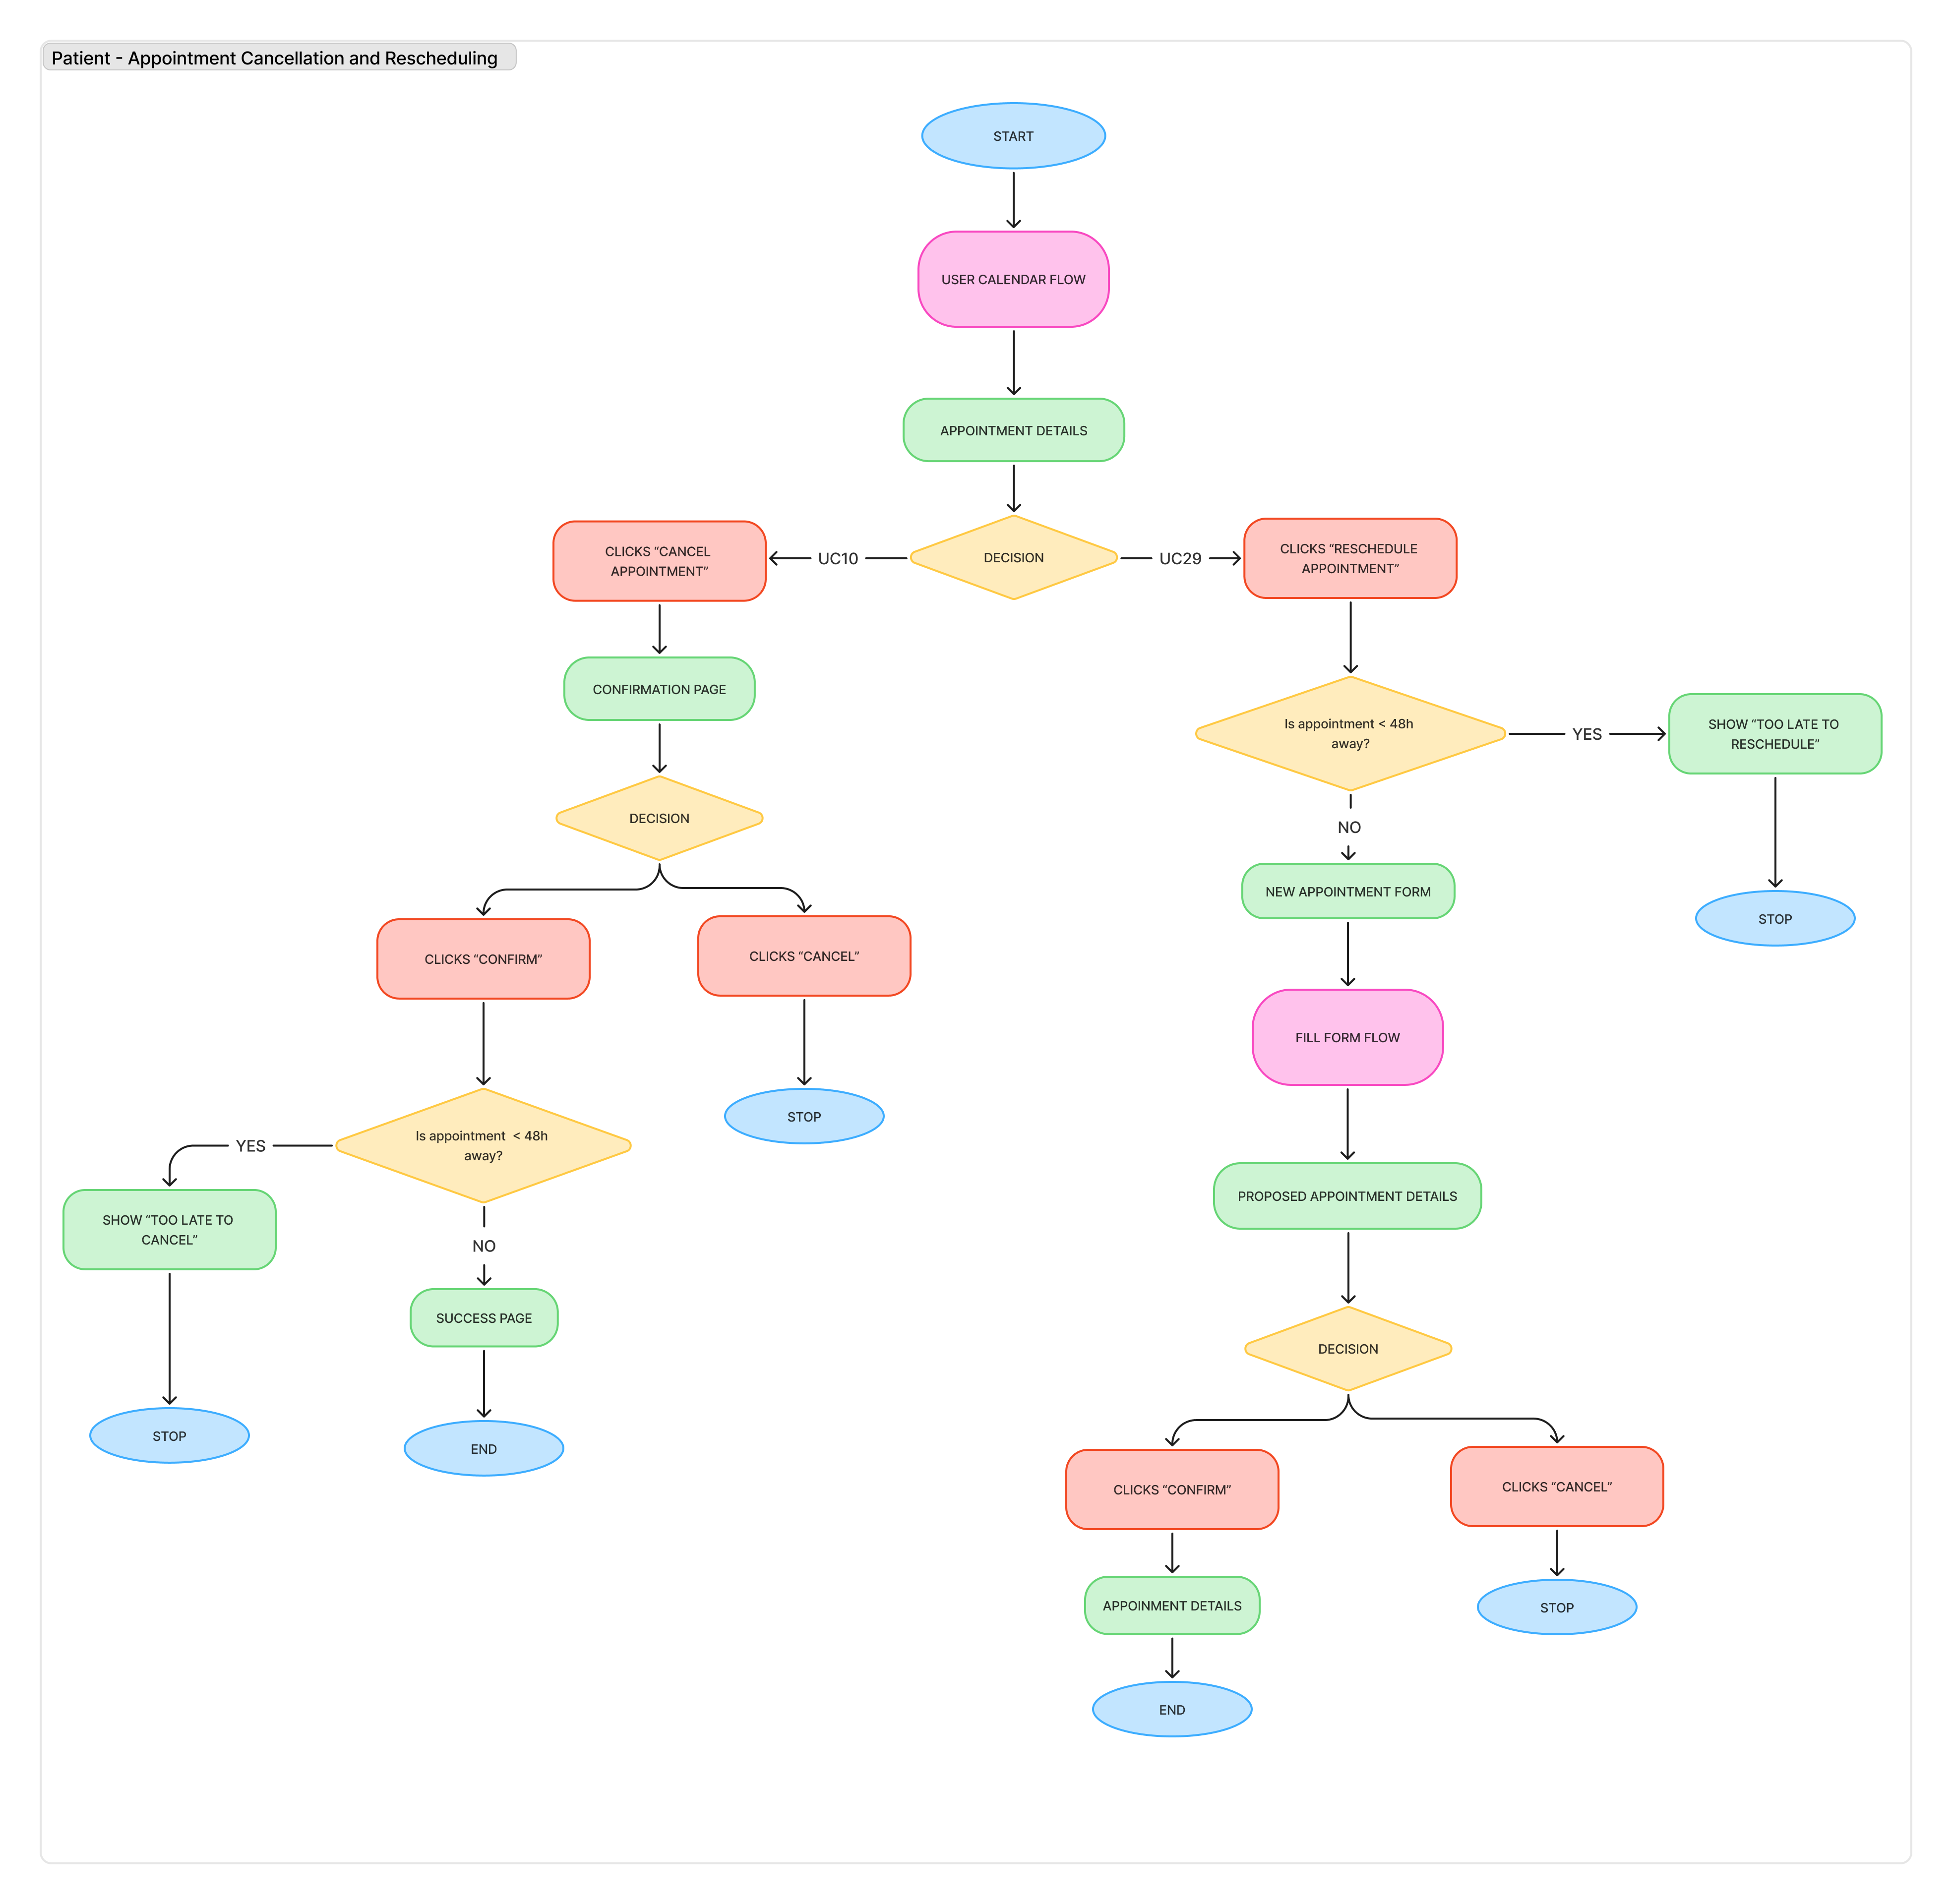
\includegraphics[width=0.8\textwidth]{User_Flows/PatientCancellationRescheduling.png}
        \captionof{figure}{User flow regarding Patient Appointment Cancellation and Rescheduling}
    \end{center}
    %\begin{itemize}   
    %\end{itemize}
\end{minipage}
\vspace{3em}

\begin{minipage}{\textwidth}
    \phantomsection
    \subsection{UF13. Patient - Appointment Booking and Payment}
    The following user flow shows the steps a patient takes to book and pay an appointment.
    It refers to use case \textbf{UC27, UC32}, and methods \textbf{bookAppointment(), ??} from the class \textbf{Patient} of the class diagram.
    
    \begin{center}
        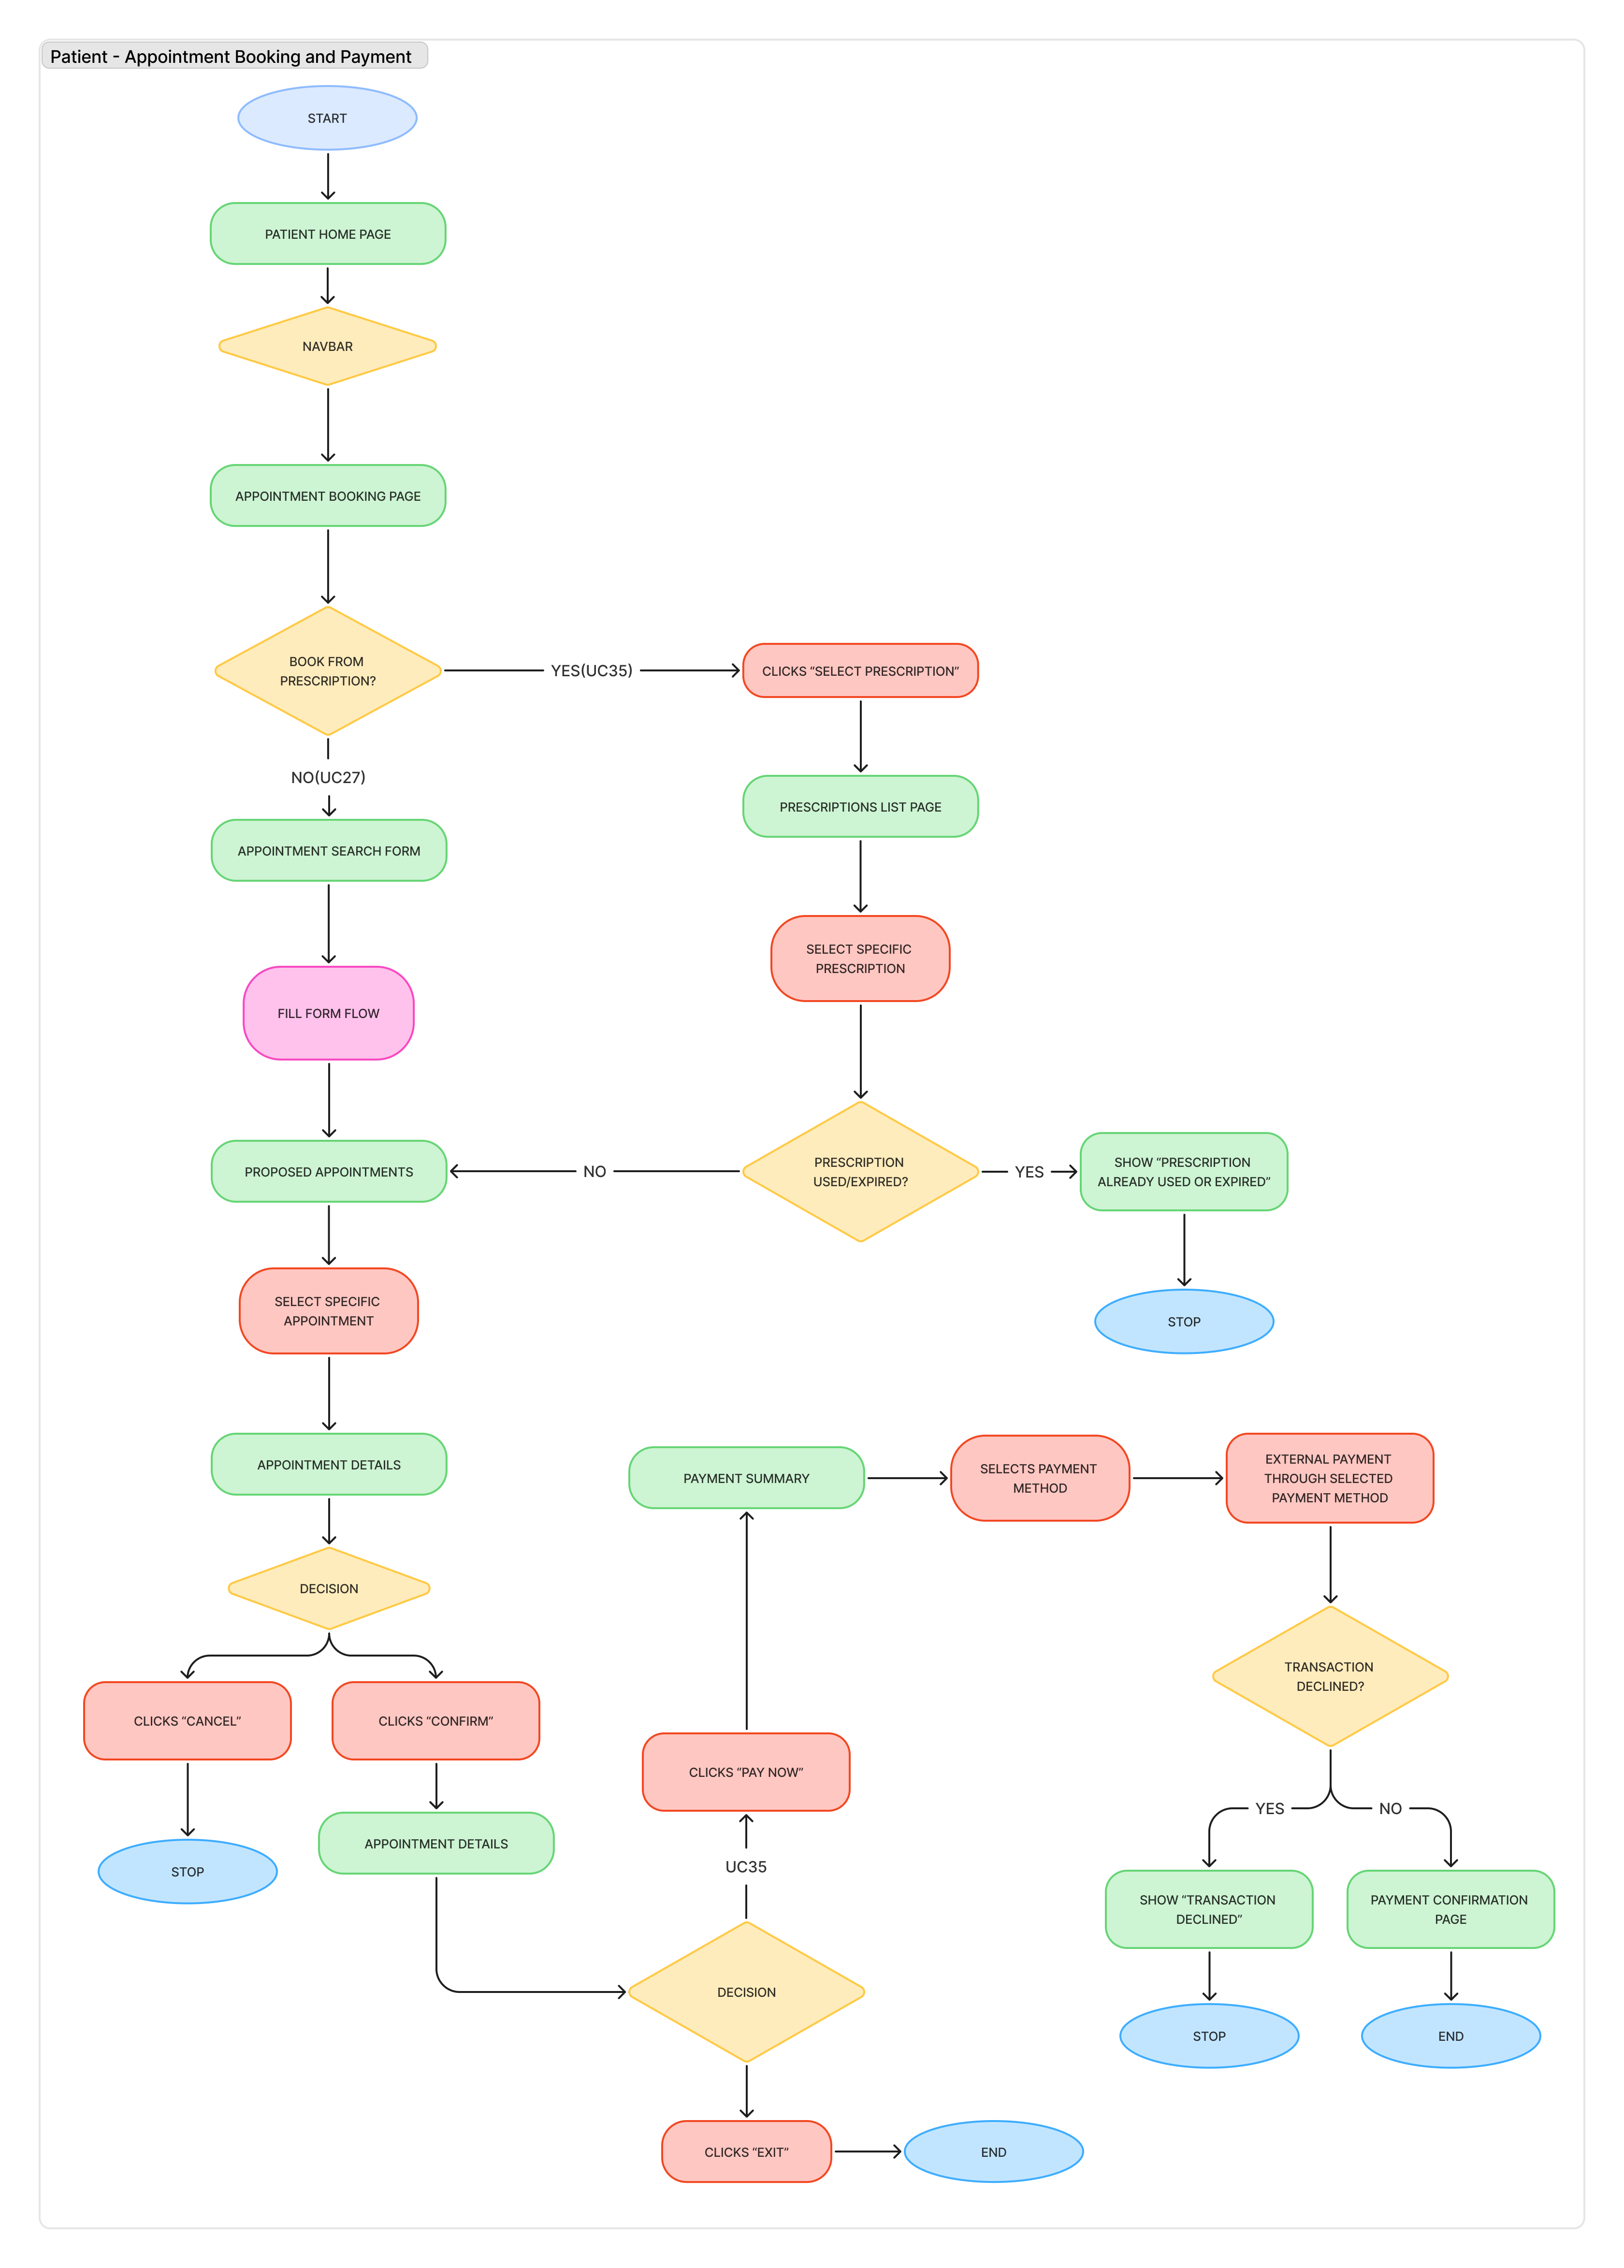
\includegraphics[width=0.8\textwidth]{User_Flows/AppointmentBookingPayment.png}
        \captionof{figure}{User flow regarding Patient Appointment Booking and Payment}
    \end{center}
    %\begin{itemize}   
    %\end{itemize}
\end{minipage}
\vspace{3em}

\begin{minipage}{\textwidth}
    \phantomsection
    \subsection{UF14. Patient - Register Insurance Policy via unique code}
    The following user flow shows the steps a patient takes to add an insurance policy to their profile via unique code.
    It refers to use case \textbf{UC36}, and methods \textbf{registerInsurance(code:String)} from the class \textbf{Patient} of the class diagram.
    
    \begin{center}
        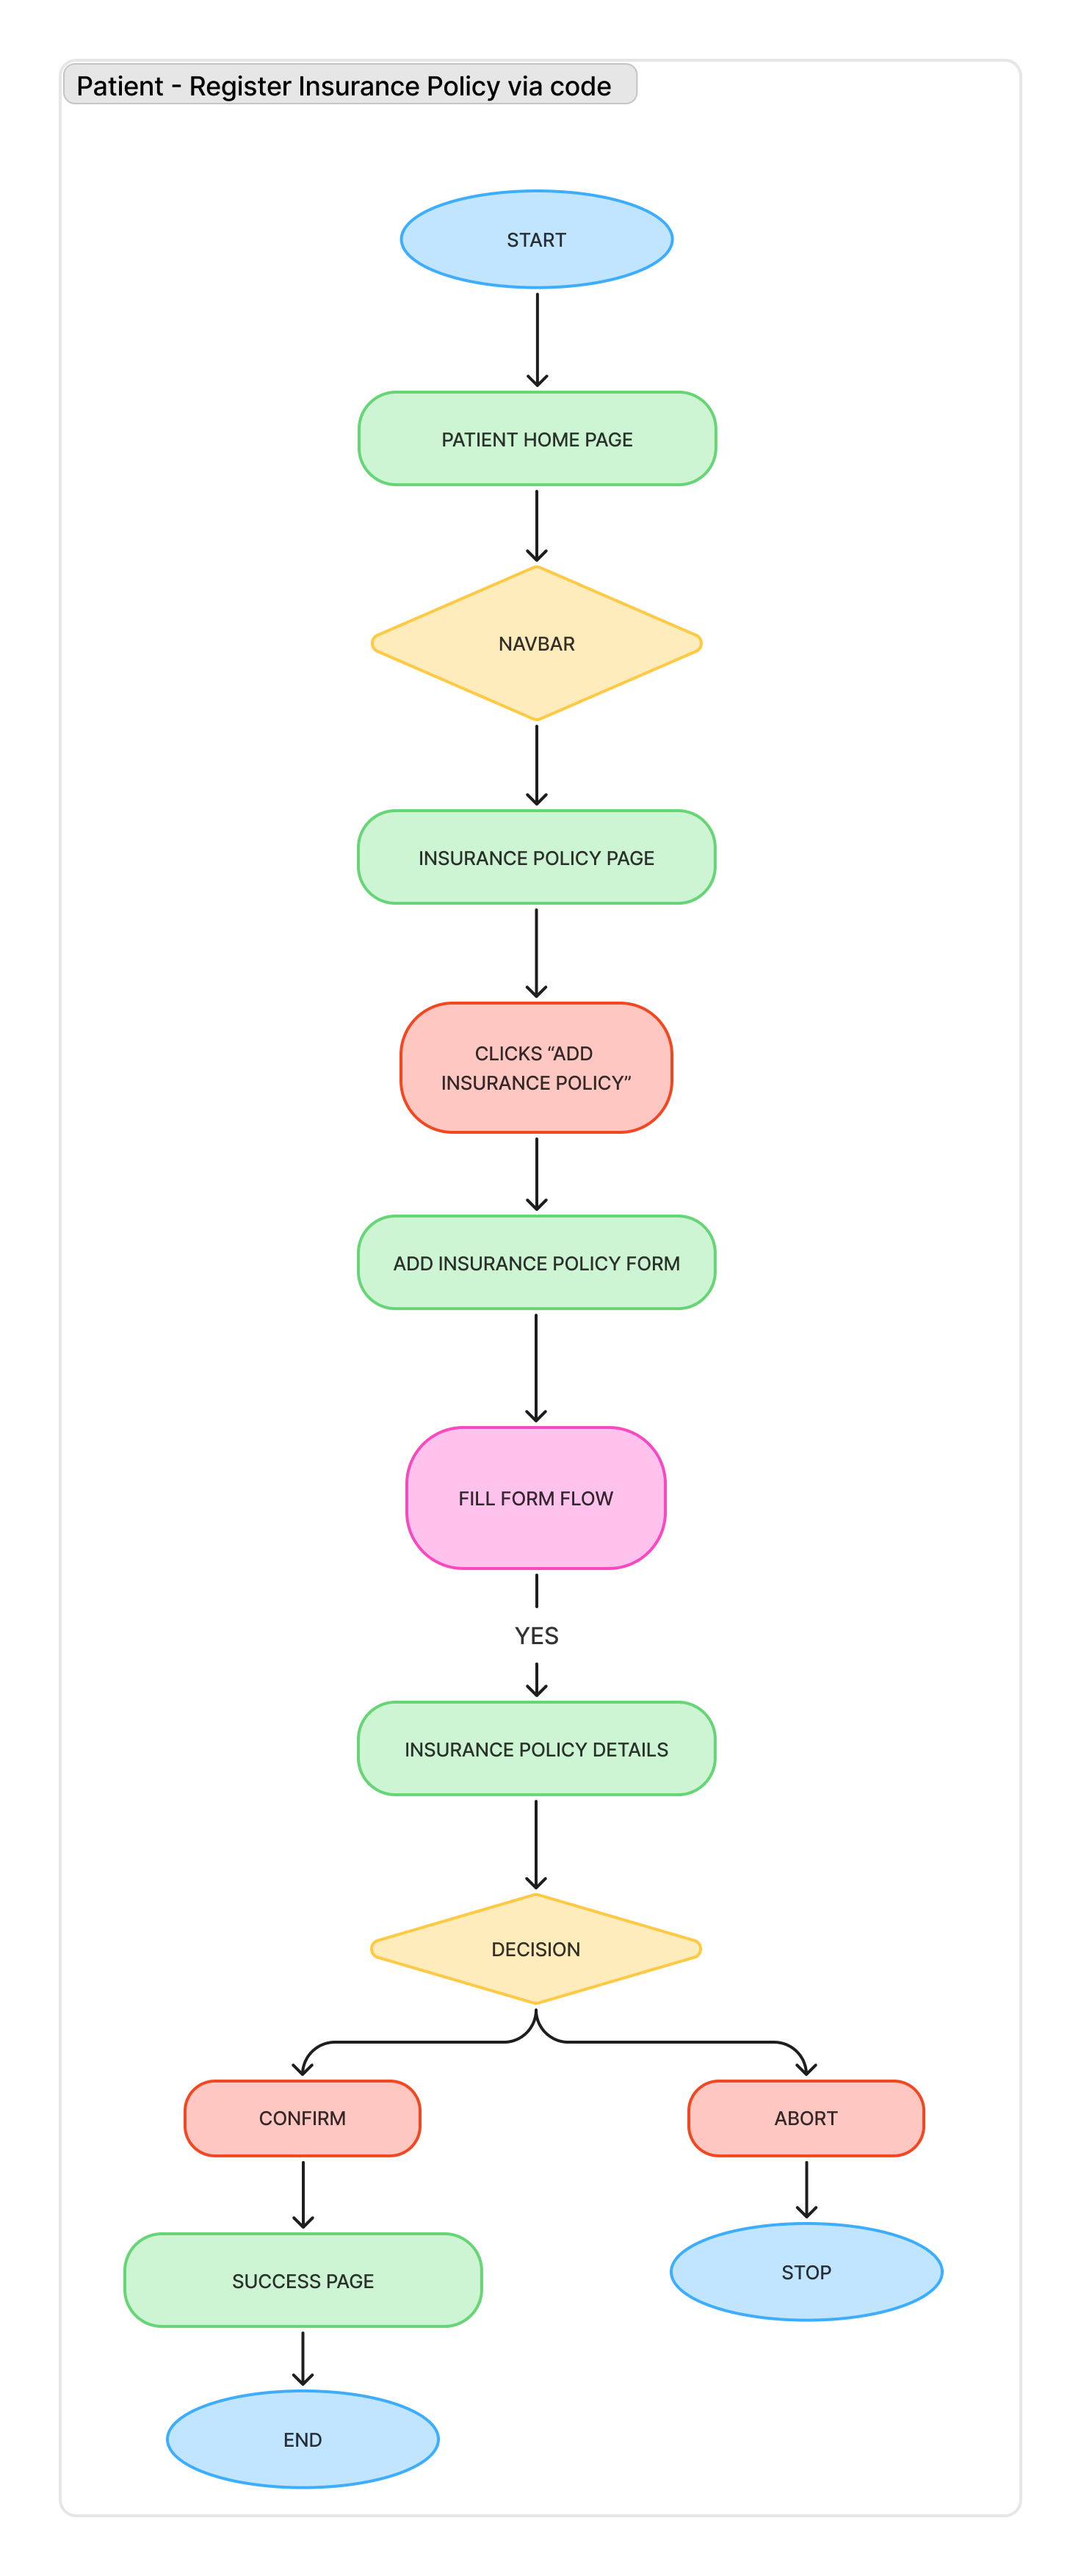
\includegraphics[width=0.5\textwidth]{User_Flows/PatientRegisterPolicy.png}
        \captionof{figure}{User flow regarding Patient Register Insurance Policy via unique code}
    \end{center}
    %\begin{itemize}   
    %\end{itemize}
\end{minipage}
\vspace{3em}

\begin{minipage}{\textwidth}
    \phantomsection
    \subsection{UF15. Patient - Medical Record and Prescriptions consultation}
    \label{UF15}
    The following user flow shows the steps a patient takes to view their medical record and prescriptions in detail.
    It refers to use case \textbf{UC38, UC39, UC40}, and methods \textbf{??} from the class \textbf{Patient} of the class diagram.
    
    \begin{center}
        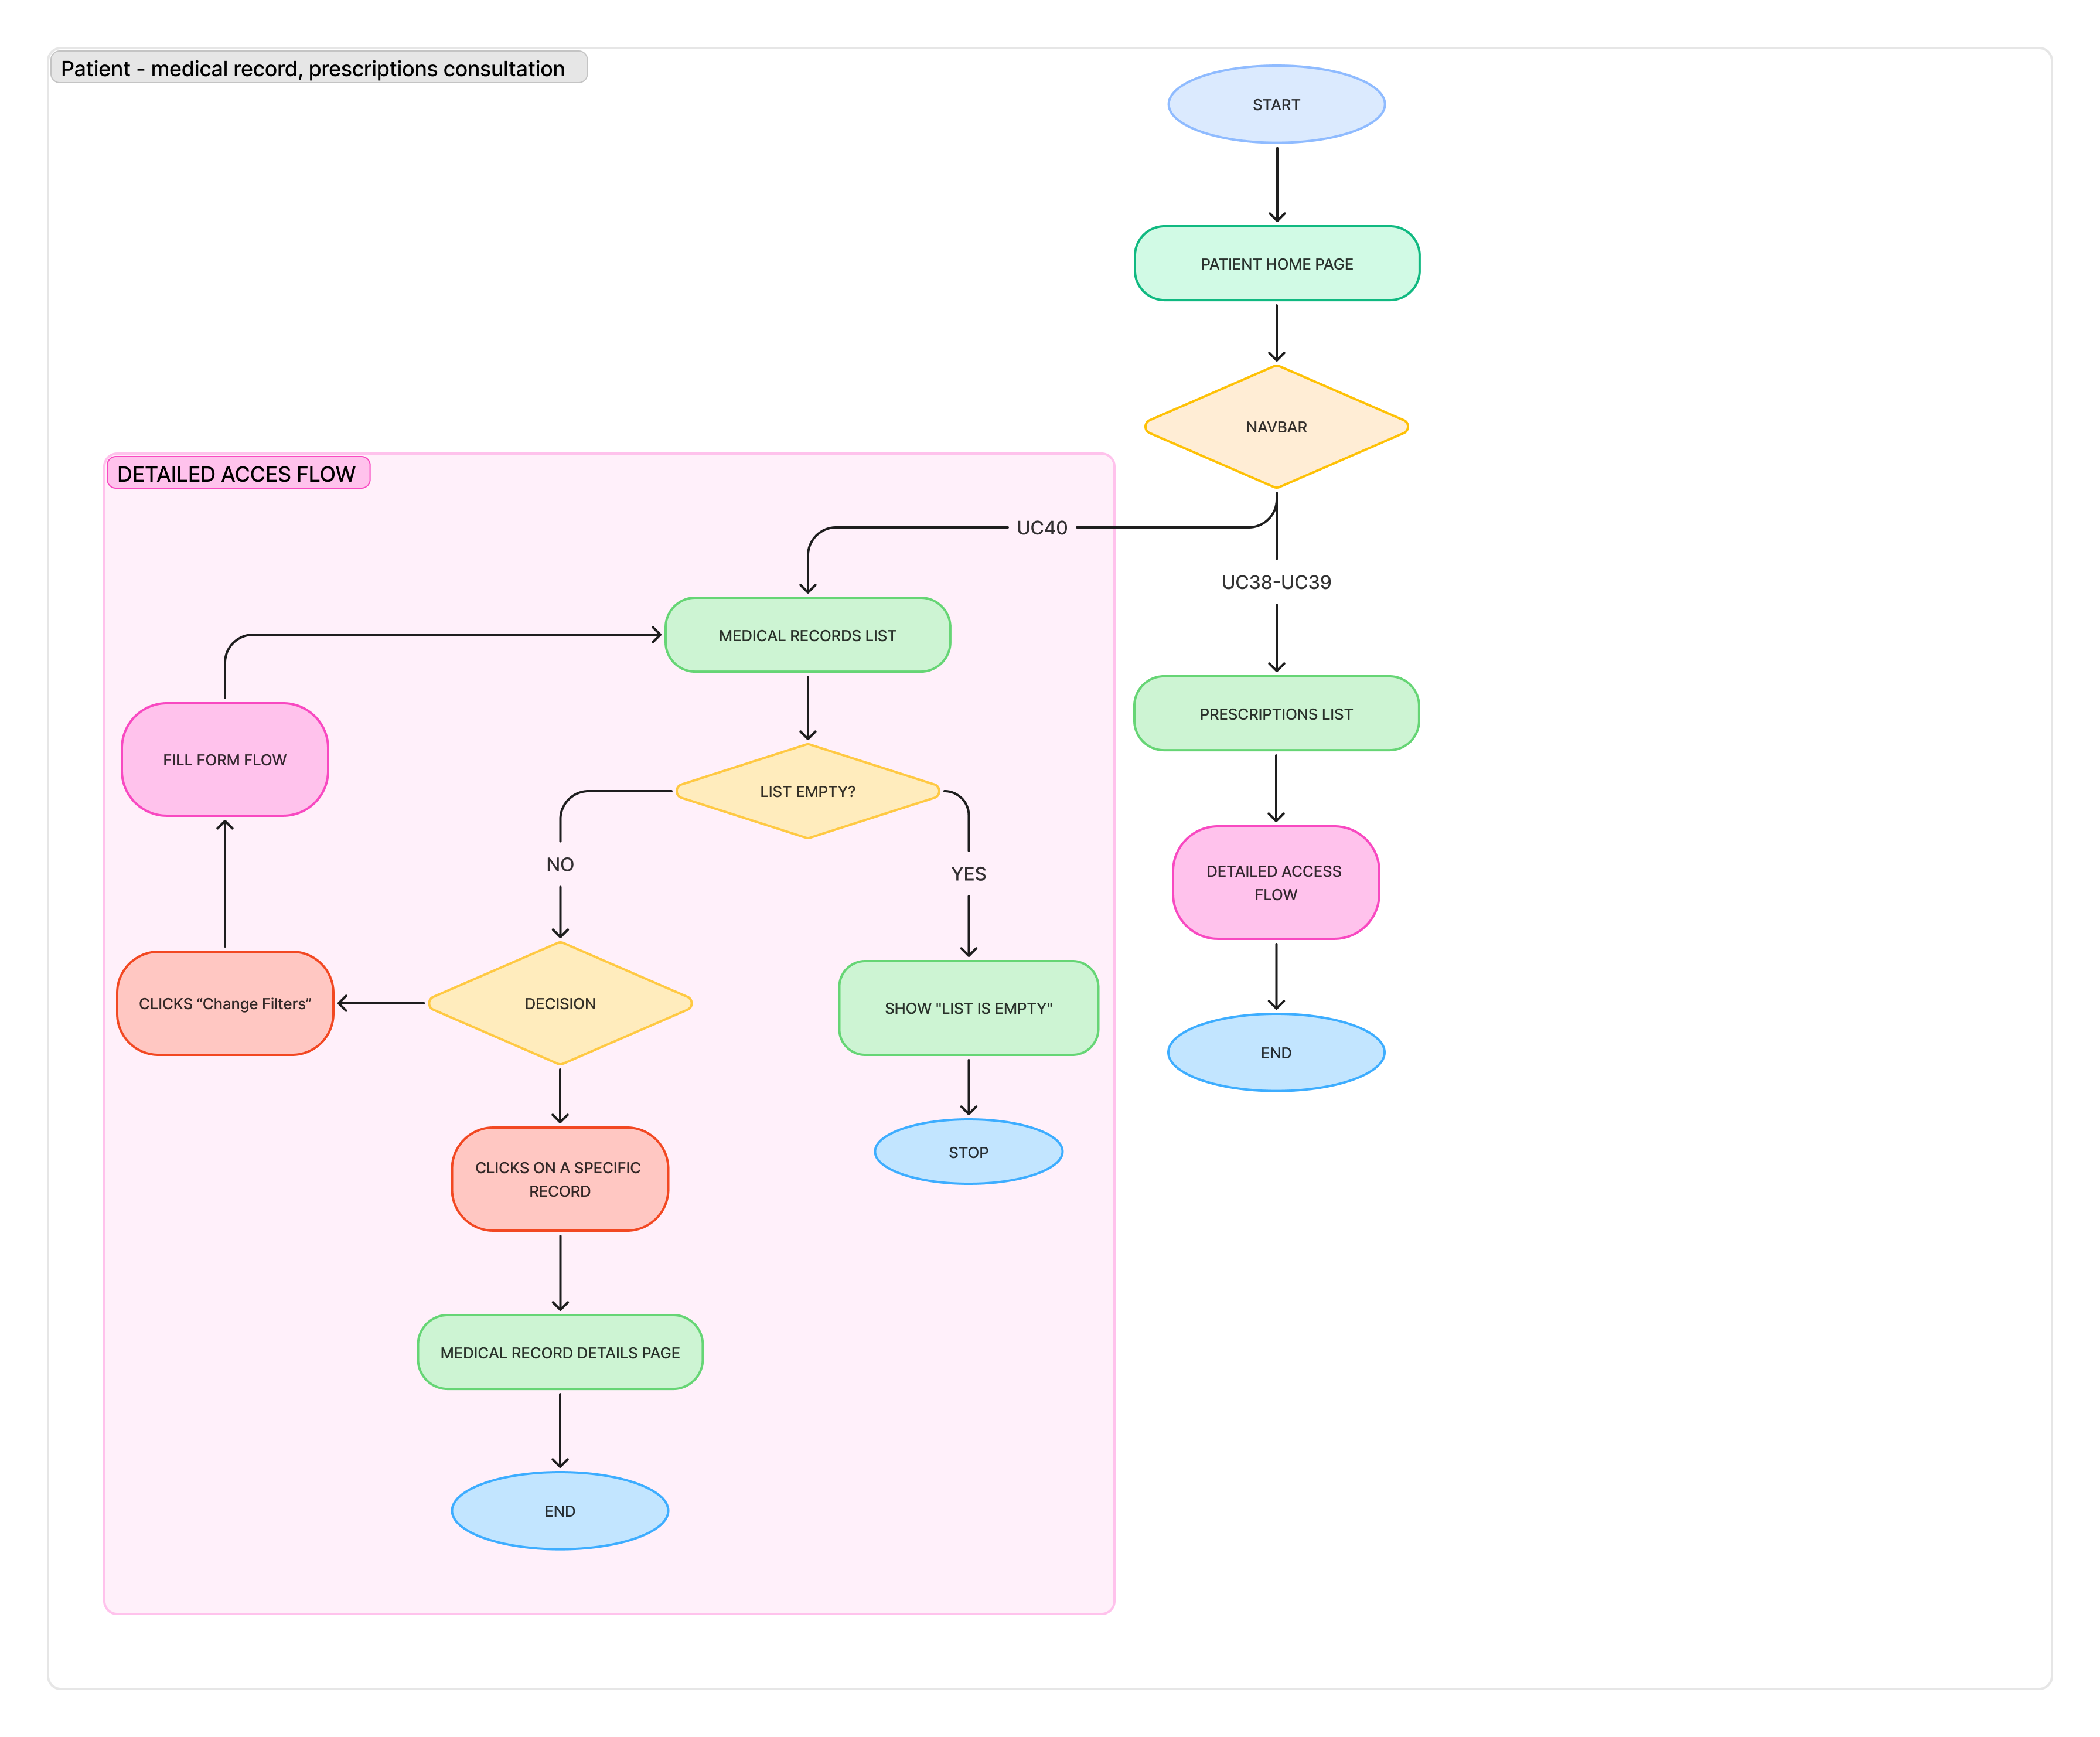
\includegraphics[width=0.9\textwidth]{User_Flows/PatientMedicalRecordPrescriptionExemptions.png}
        \captionof{figure}{User flow regarding Patient Medical Record and Prescriptions consultation}
    \end{center}
    %\begin{itemize}   
    %\end{itemize}
\end{minipage}
\vspace{3em}

\begin{minipage}{\textwidth}
    \phantomsection
    \subsection{UF16. Doctor - Access Patient's Medical Record, Chronological Report}
    The following user flow shows the steps a doctor takes to access a patient's medical records and to consult their own chronological report.
    It refers to use case \textbf{UC42, UC43}, and methods \textbf{accessPatientRecord(),viewChronologicalReport()} from the class \textbf{Doctor} of the class diagram.
    
    \begin{center}
        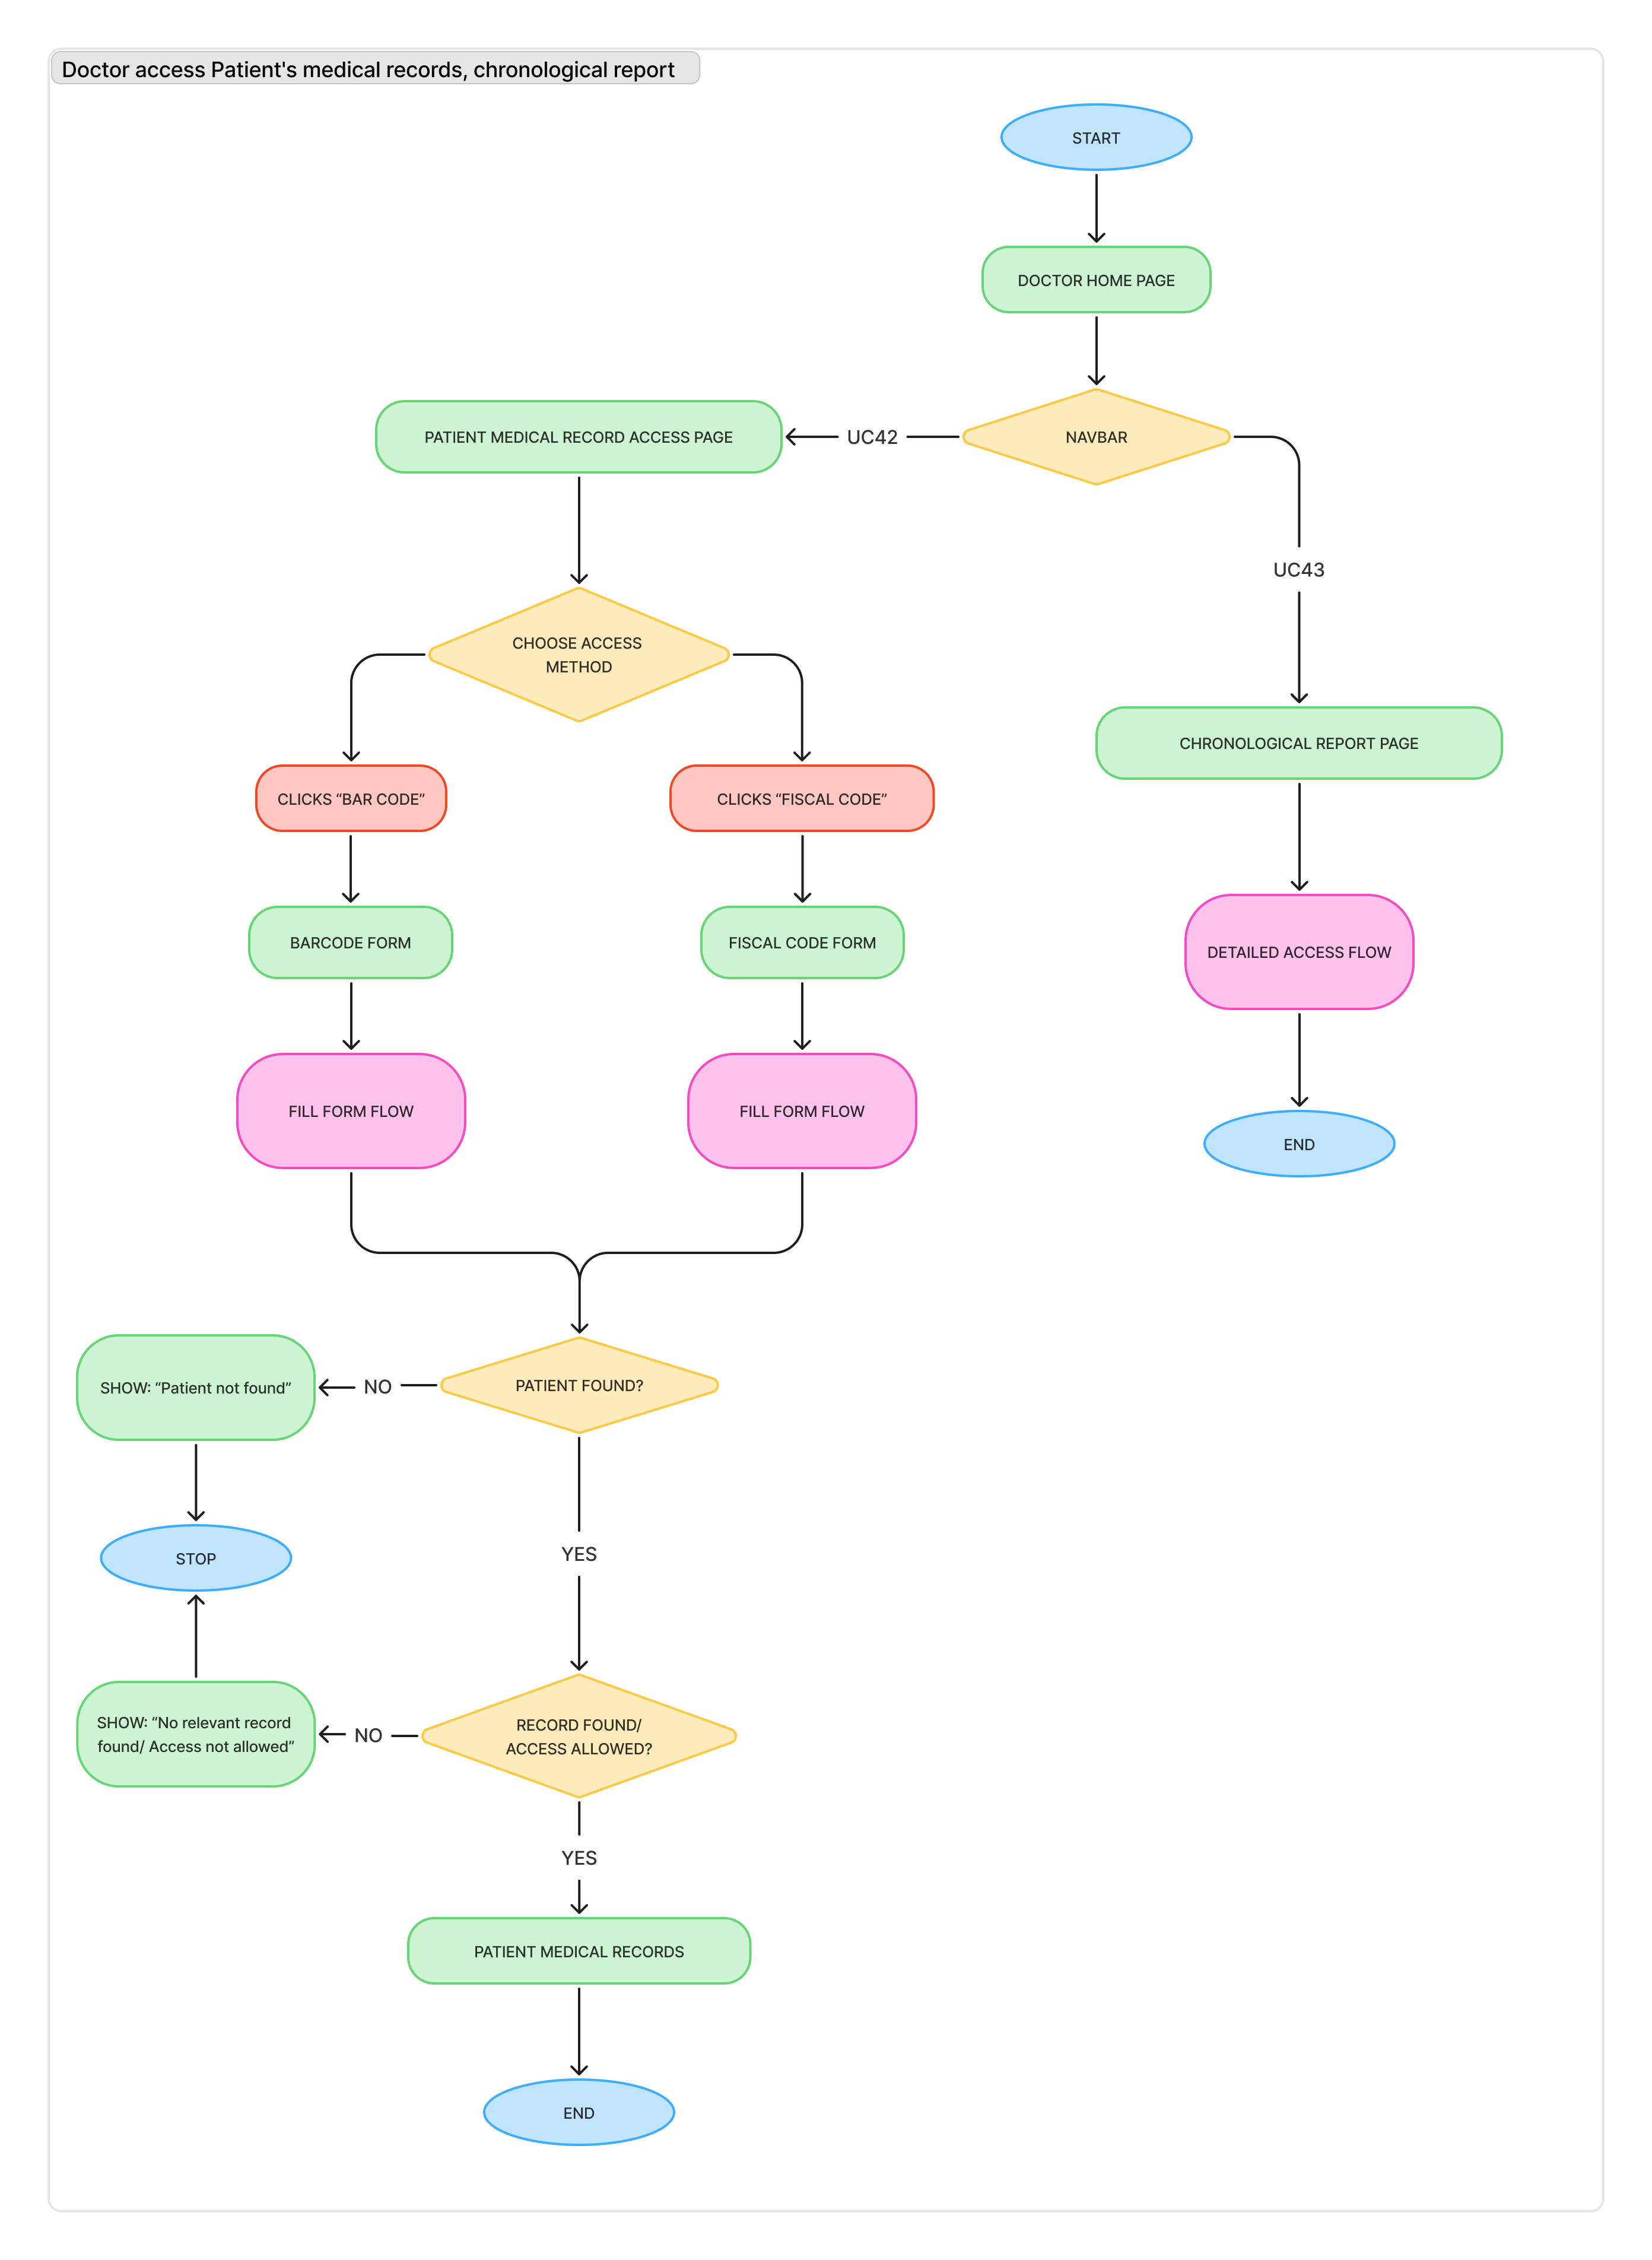
\includegraphics[width=0.9\textwidth]{User_Flows/DoctorMedicalRecordReport.png}
        \captionof{figure}{User flow regarding Doctor Access Patient's Medical Record, Chronological Report}
    \end{center}
    %\begin{itemize}   
    %\end{itemize}
\end{minipage}
\vspace{3em}

\begin{minipage}{\textwidth}
    \phantomsection
    \subsection{UF17. Doctor - Upload Prescriptions, Exemptions and Exam Results}
    The following user flow shows the steps a doctor takes to upload prescriptions, exemptions and exam result to a patient's profile.
    It refers to use case \textbf{UC3, UC4}, and methods \textbf{createPrescription(),createExemption(), uploadExamination()} from the class \textbf{Doctor} of the class diagram.
    
    \begin{center}
        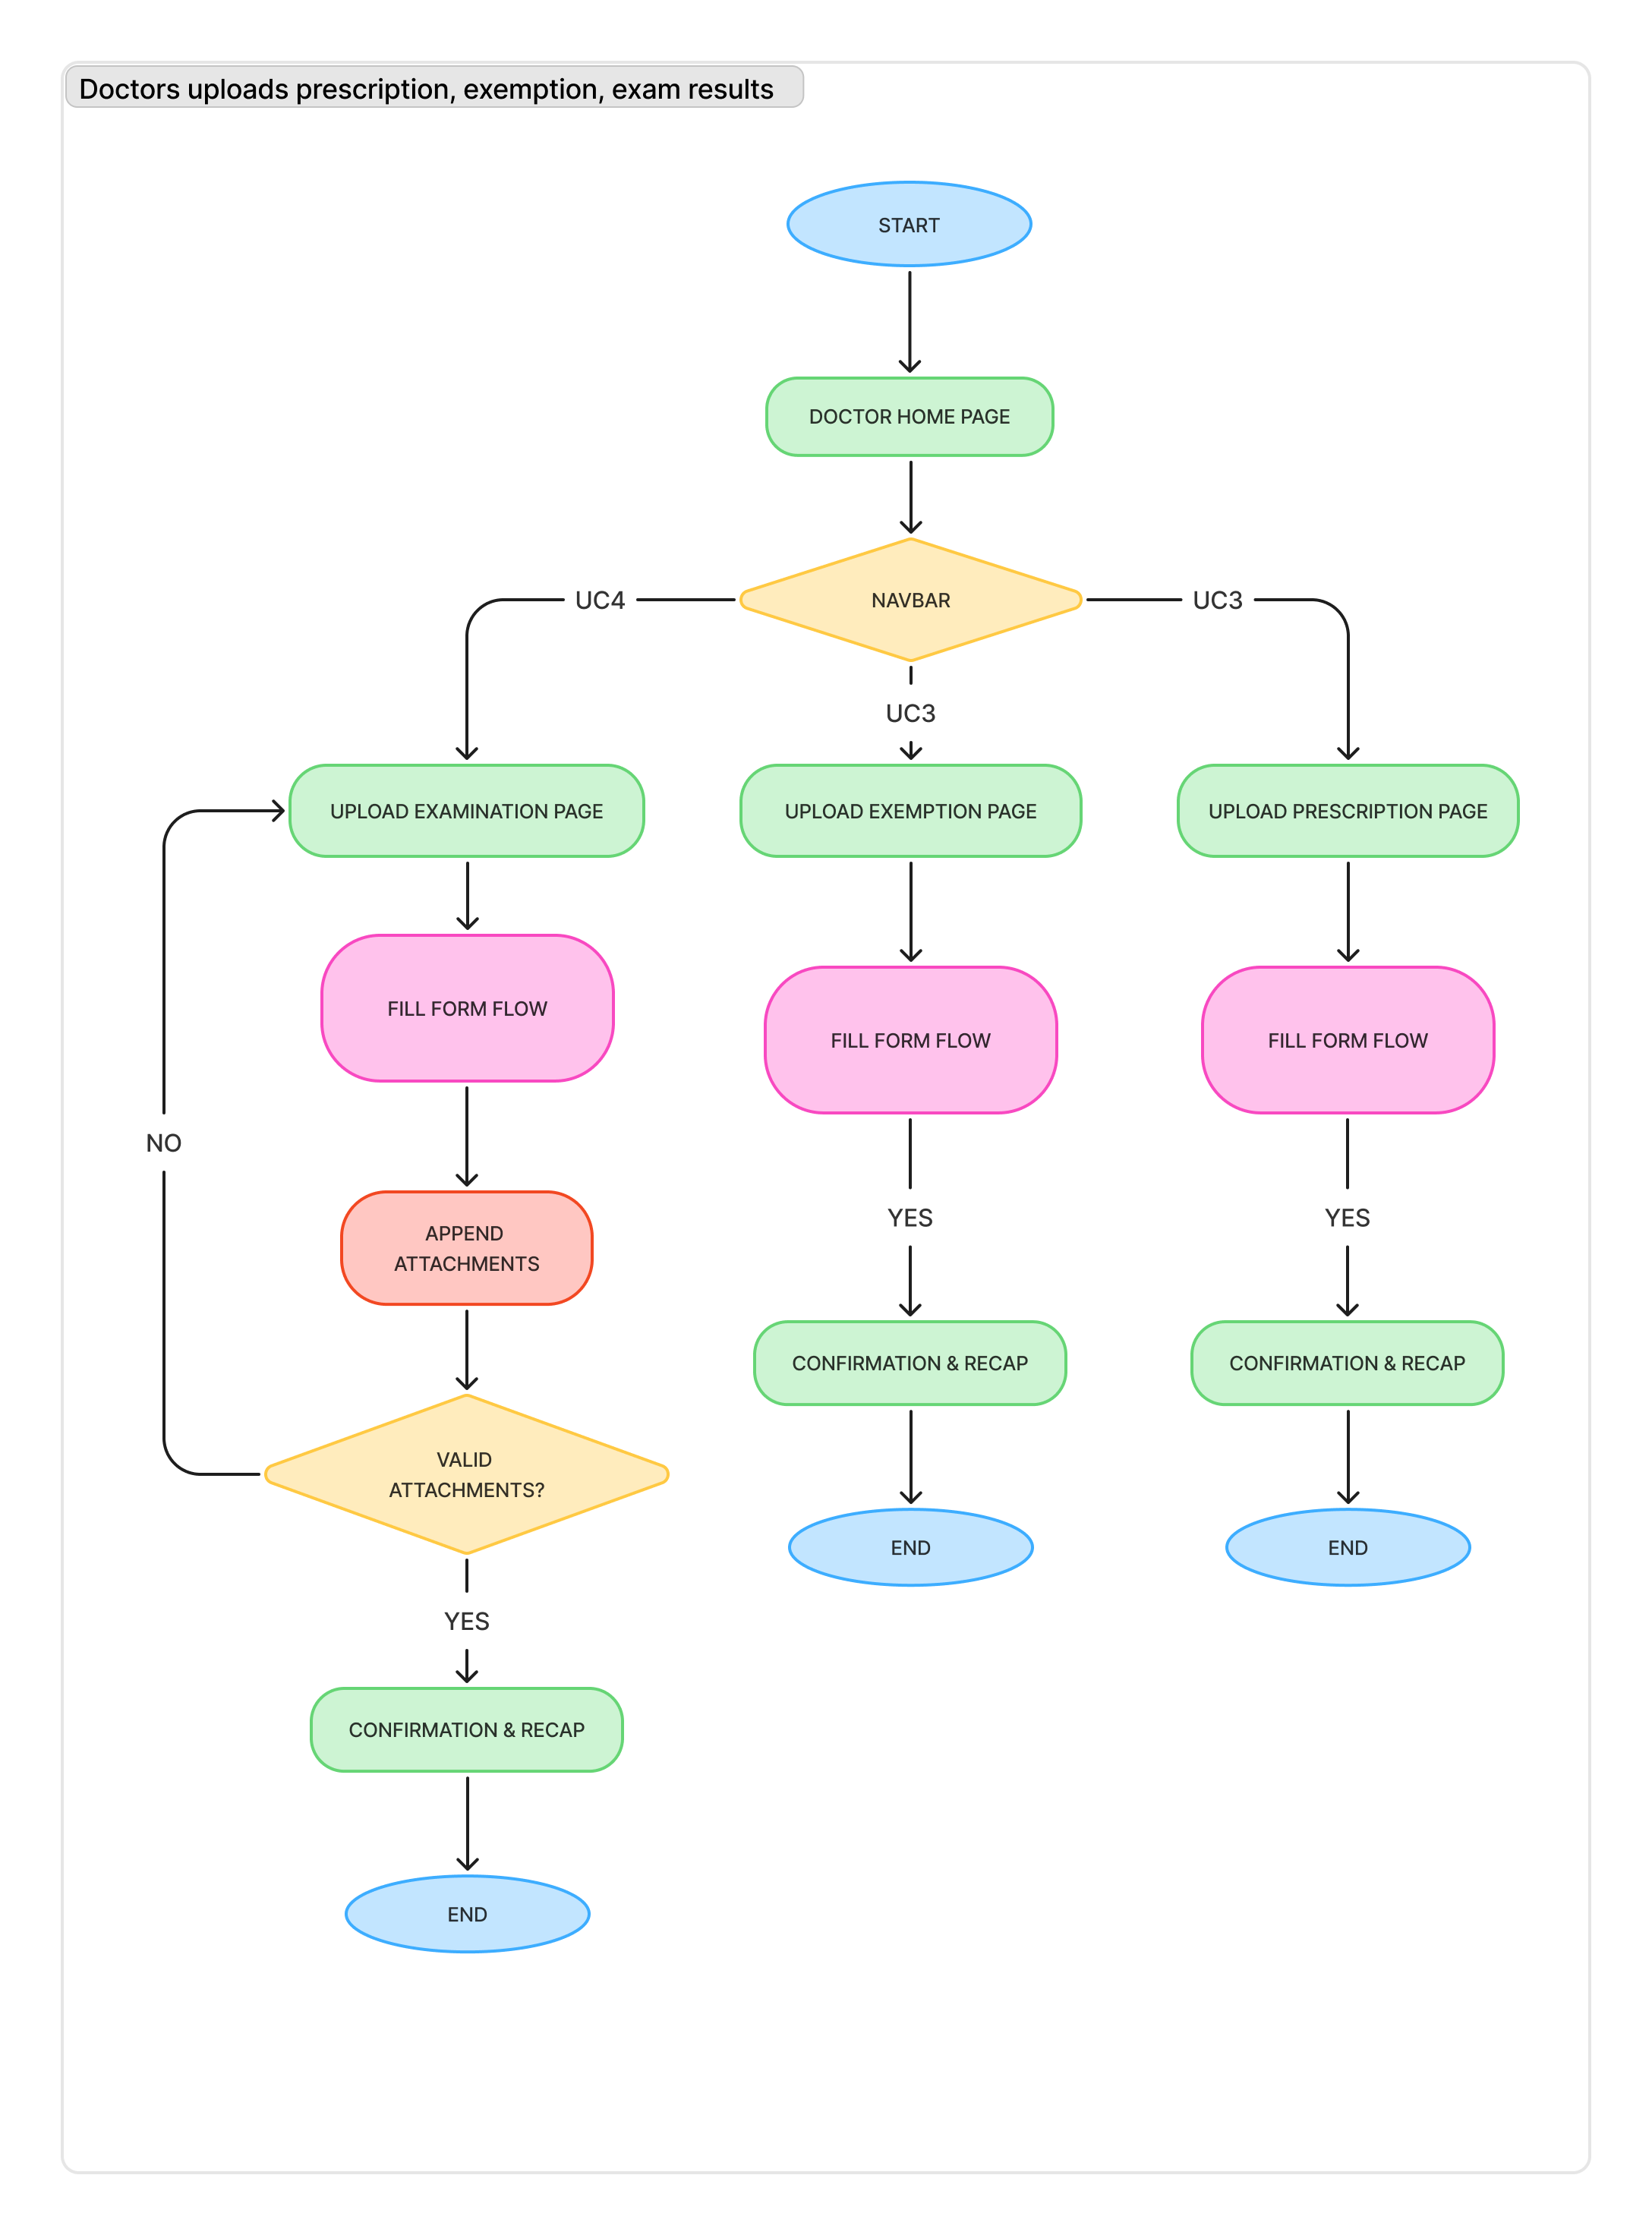
\includegraphics[width=0.9\textwidth]{User_Flows/DoctorUploads.png}
        \captionof{figure}{User flow regarding Doctor Upload Prescriptions, Exemptions and Exam Results}
    \end{center}
    %\begin{itemize}   
    %\end{itemize}
\end{minipage}
\vspace{3em}

\begin{minipage}{\textwidth}
    \phantomsection
    \subsection{UF18. Doctor - Upload Prescriptions, Exemptions and Exam Results}
    The following user flow shows the steps a doctor takes to upload prescriptions, exemptions and exam result to a patient's profile.
    It refers to use case \textbf{UC3, UC4}, and methods \textbf{createPrescription(),createExemption(), uploadExamination()} from the class \textbf{Doctor} of the class diagram.
    
    \begin{center}
        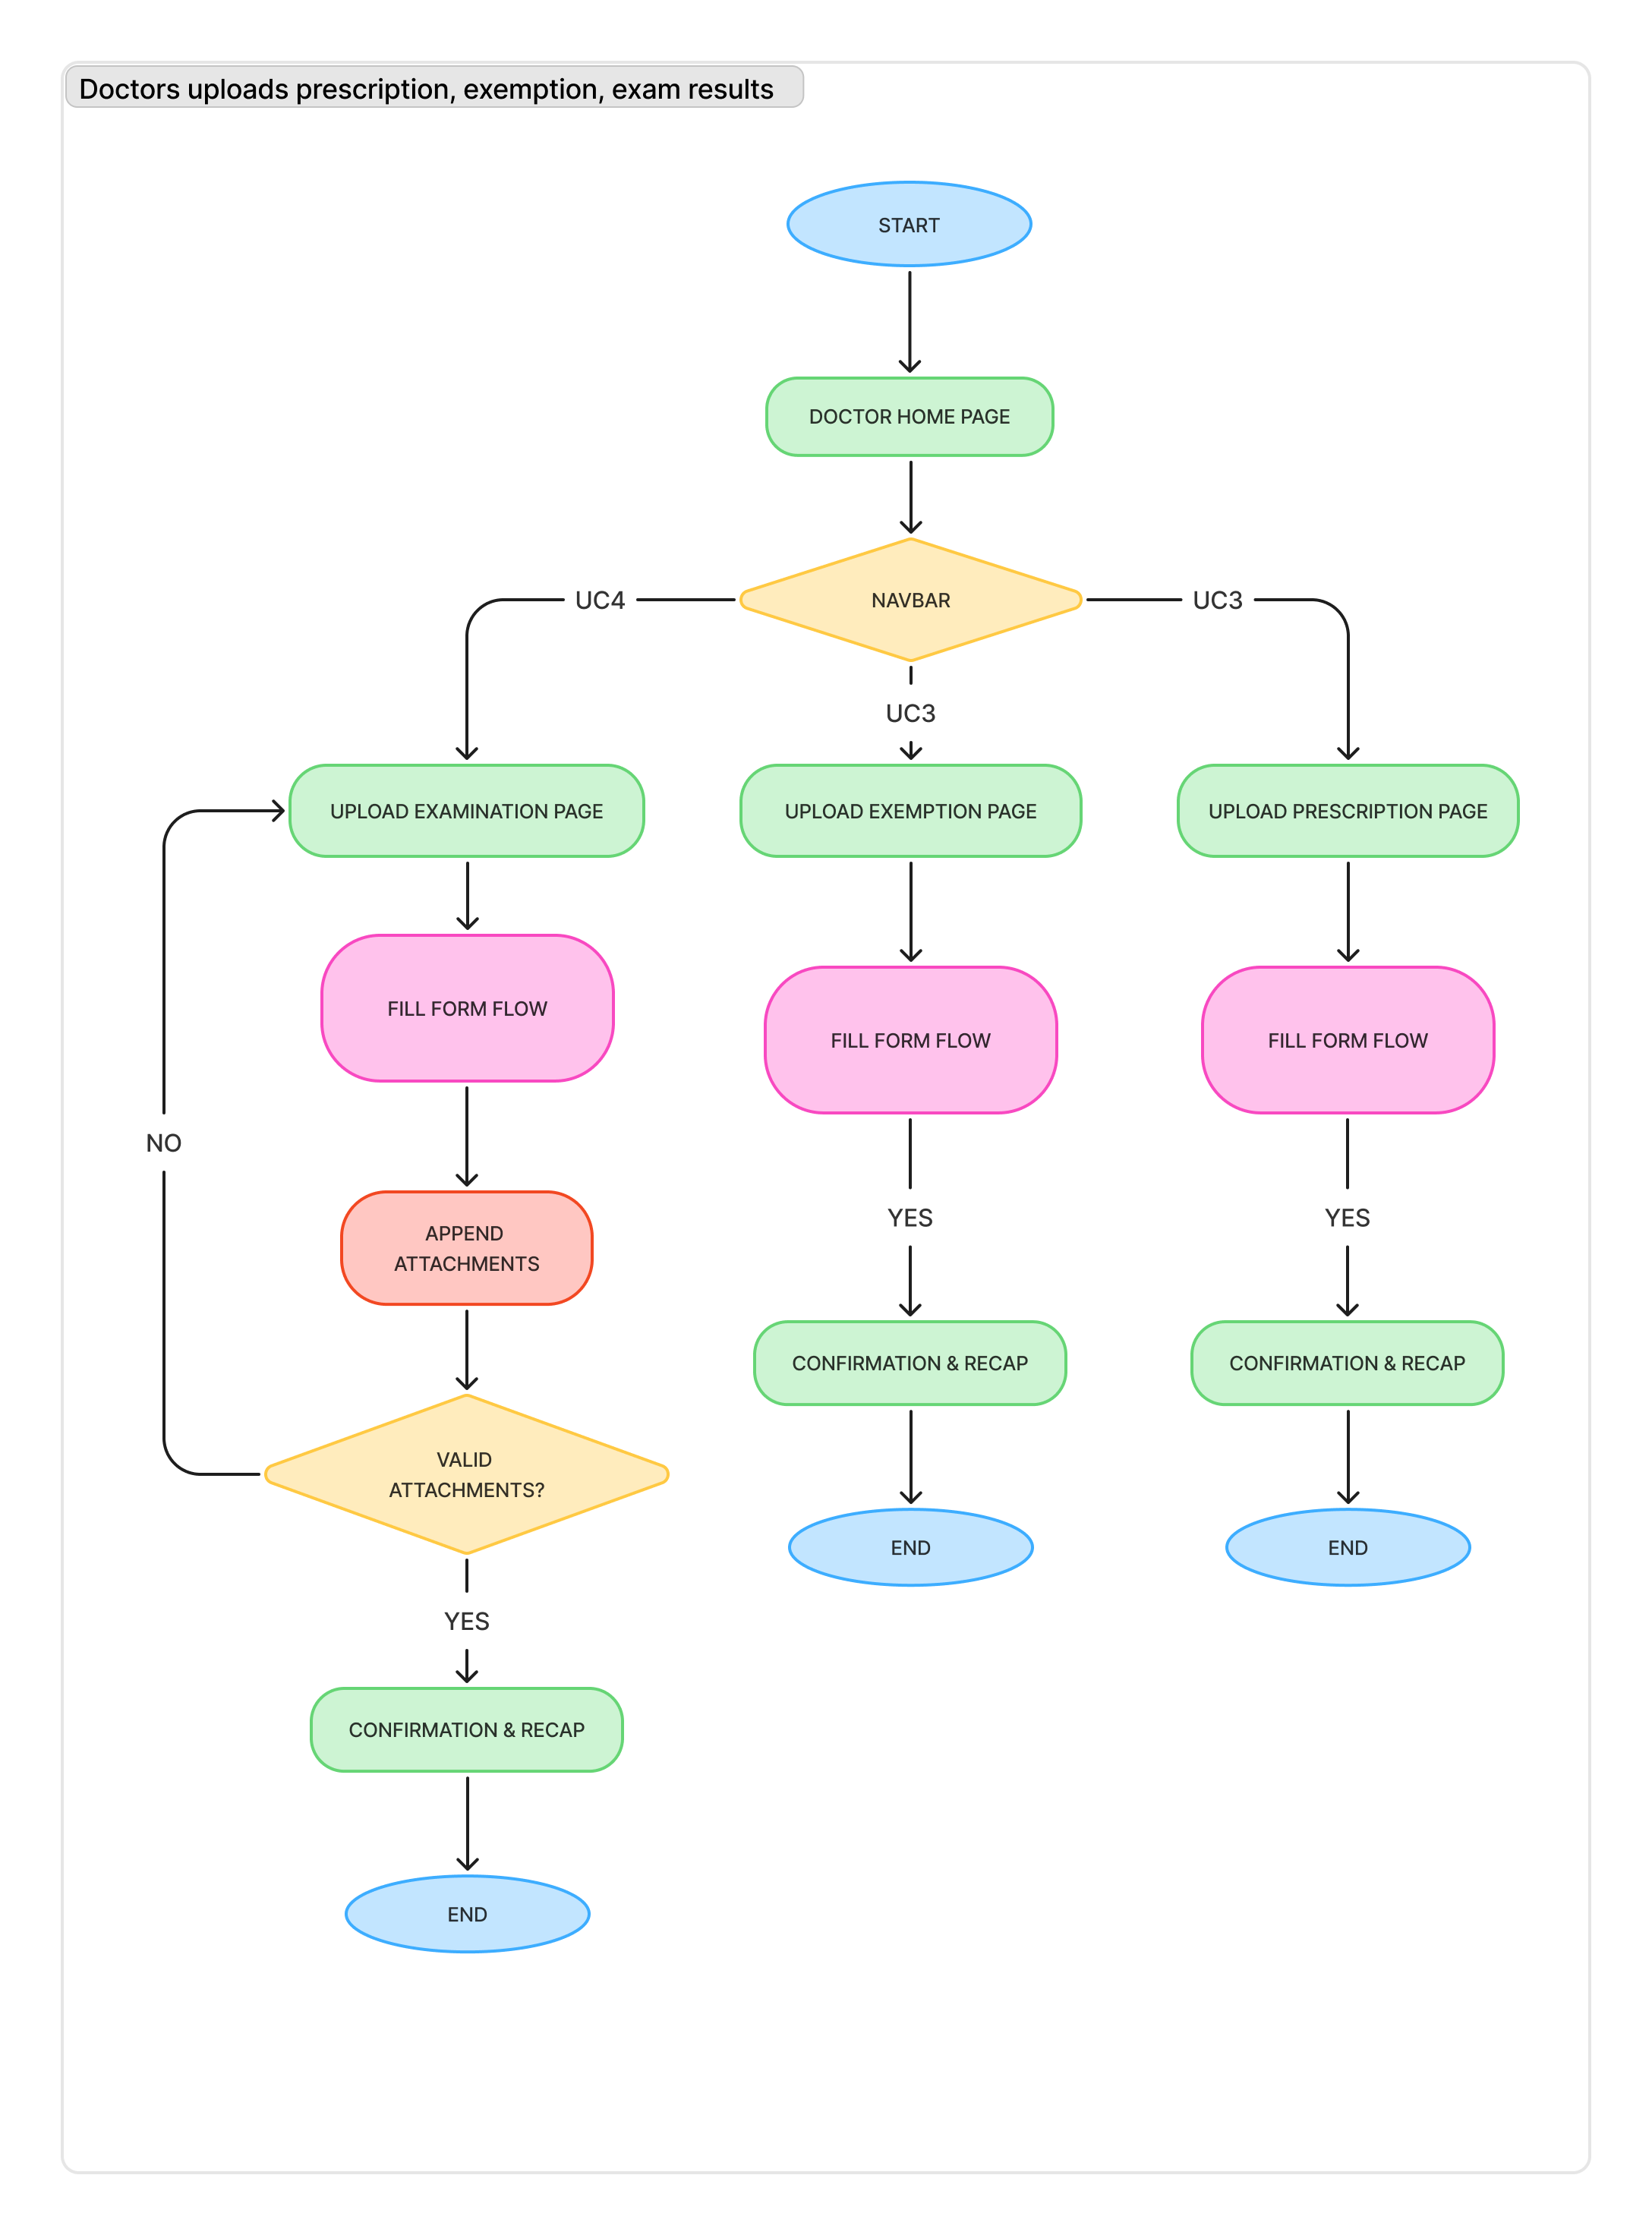
\includegraphics[width=0.9\textwidth]{User_Flows/DoctorUploads.png}
        \captionof{figure}{User flow regarding Doctor Upload Prescriptions, Exemptions and Exam Results}
    \end{center}
    %\begin{itemize}   
    %\end{itemize}
\end{minipage}
\vspace{3em}

\begin{minipage}{\textwidth}
    \phantomsection
    \subsection{UF19. Doctor - Cancel Appointment}
    The following user flow shows the steps a doctor takes to cancel one of their booked examinations.
    It refers to use case \textbf{UC11}, and methods \textbf{cancelAppointment(reason : String)} from the class \textbf{Doctor} of the class diagram.
    
    \begin{center}
        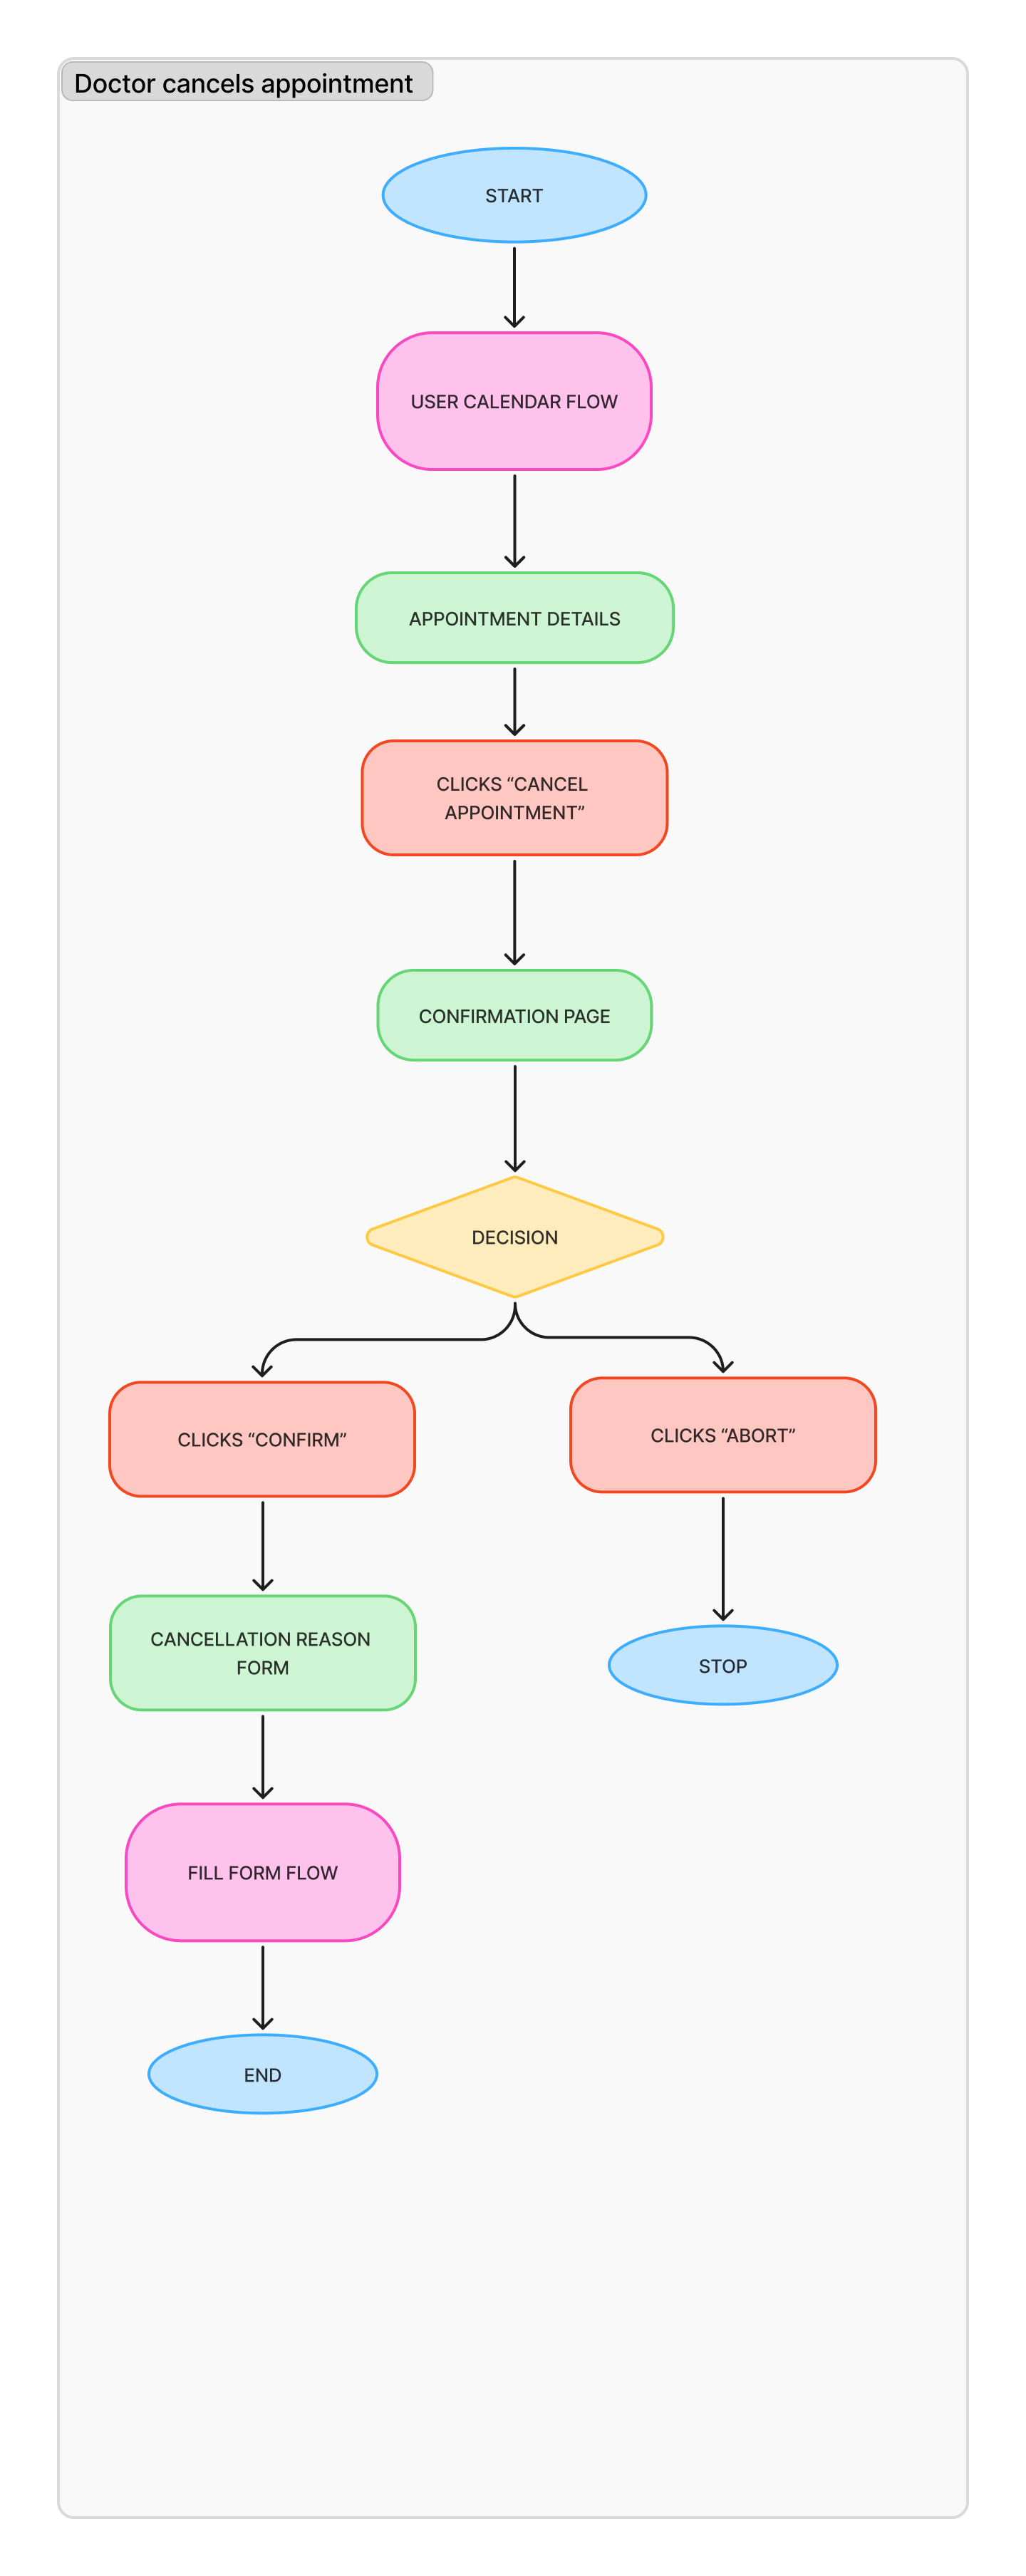
\includegraphics[width=0.9\textwidth]{User_Flows/DoctorAppointmentCancellation.png}
        \captionof{figure}{User flow regarding Doctor Appointment Cancellation}
    \end{center}
    %\begin{itemize}   
    %\end{itemize}
\end{minipage}
\vspace{3em}

\begin{minipage}{\textwidth}
    \phantomsection
    \subsection{UF20. Head of Department - Management Operations}
    The following user flow shows the steps a head of department takes to configure their department's services, capacity and doctor's workshifts.
    It refers to use case \textbf{UC17, UC21, UC44}, and methods \textbf{updateDepartmentTreatments(), configureDepartmentCapacity(),  setShiftPattern(doctor : Doctor)} from the class \textbf{Head of Department} of the class diagram.
    
    \begin{center}
        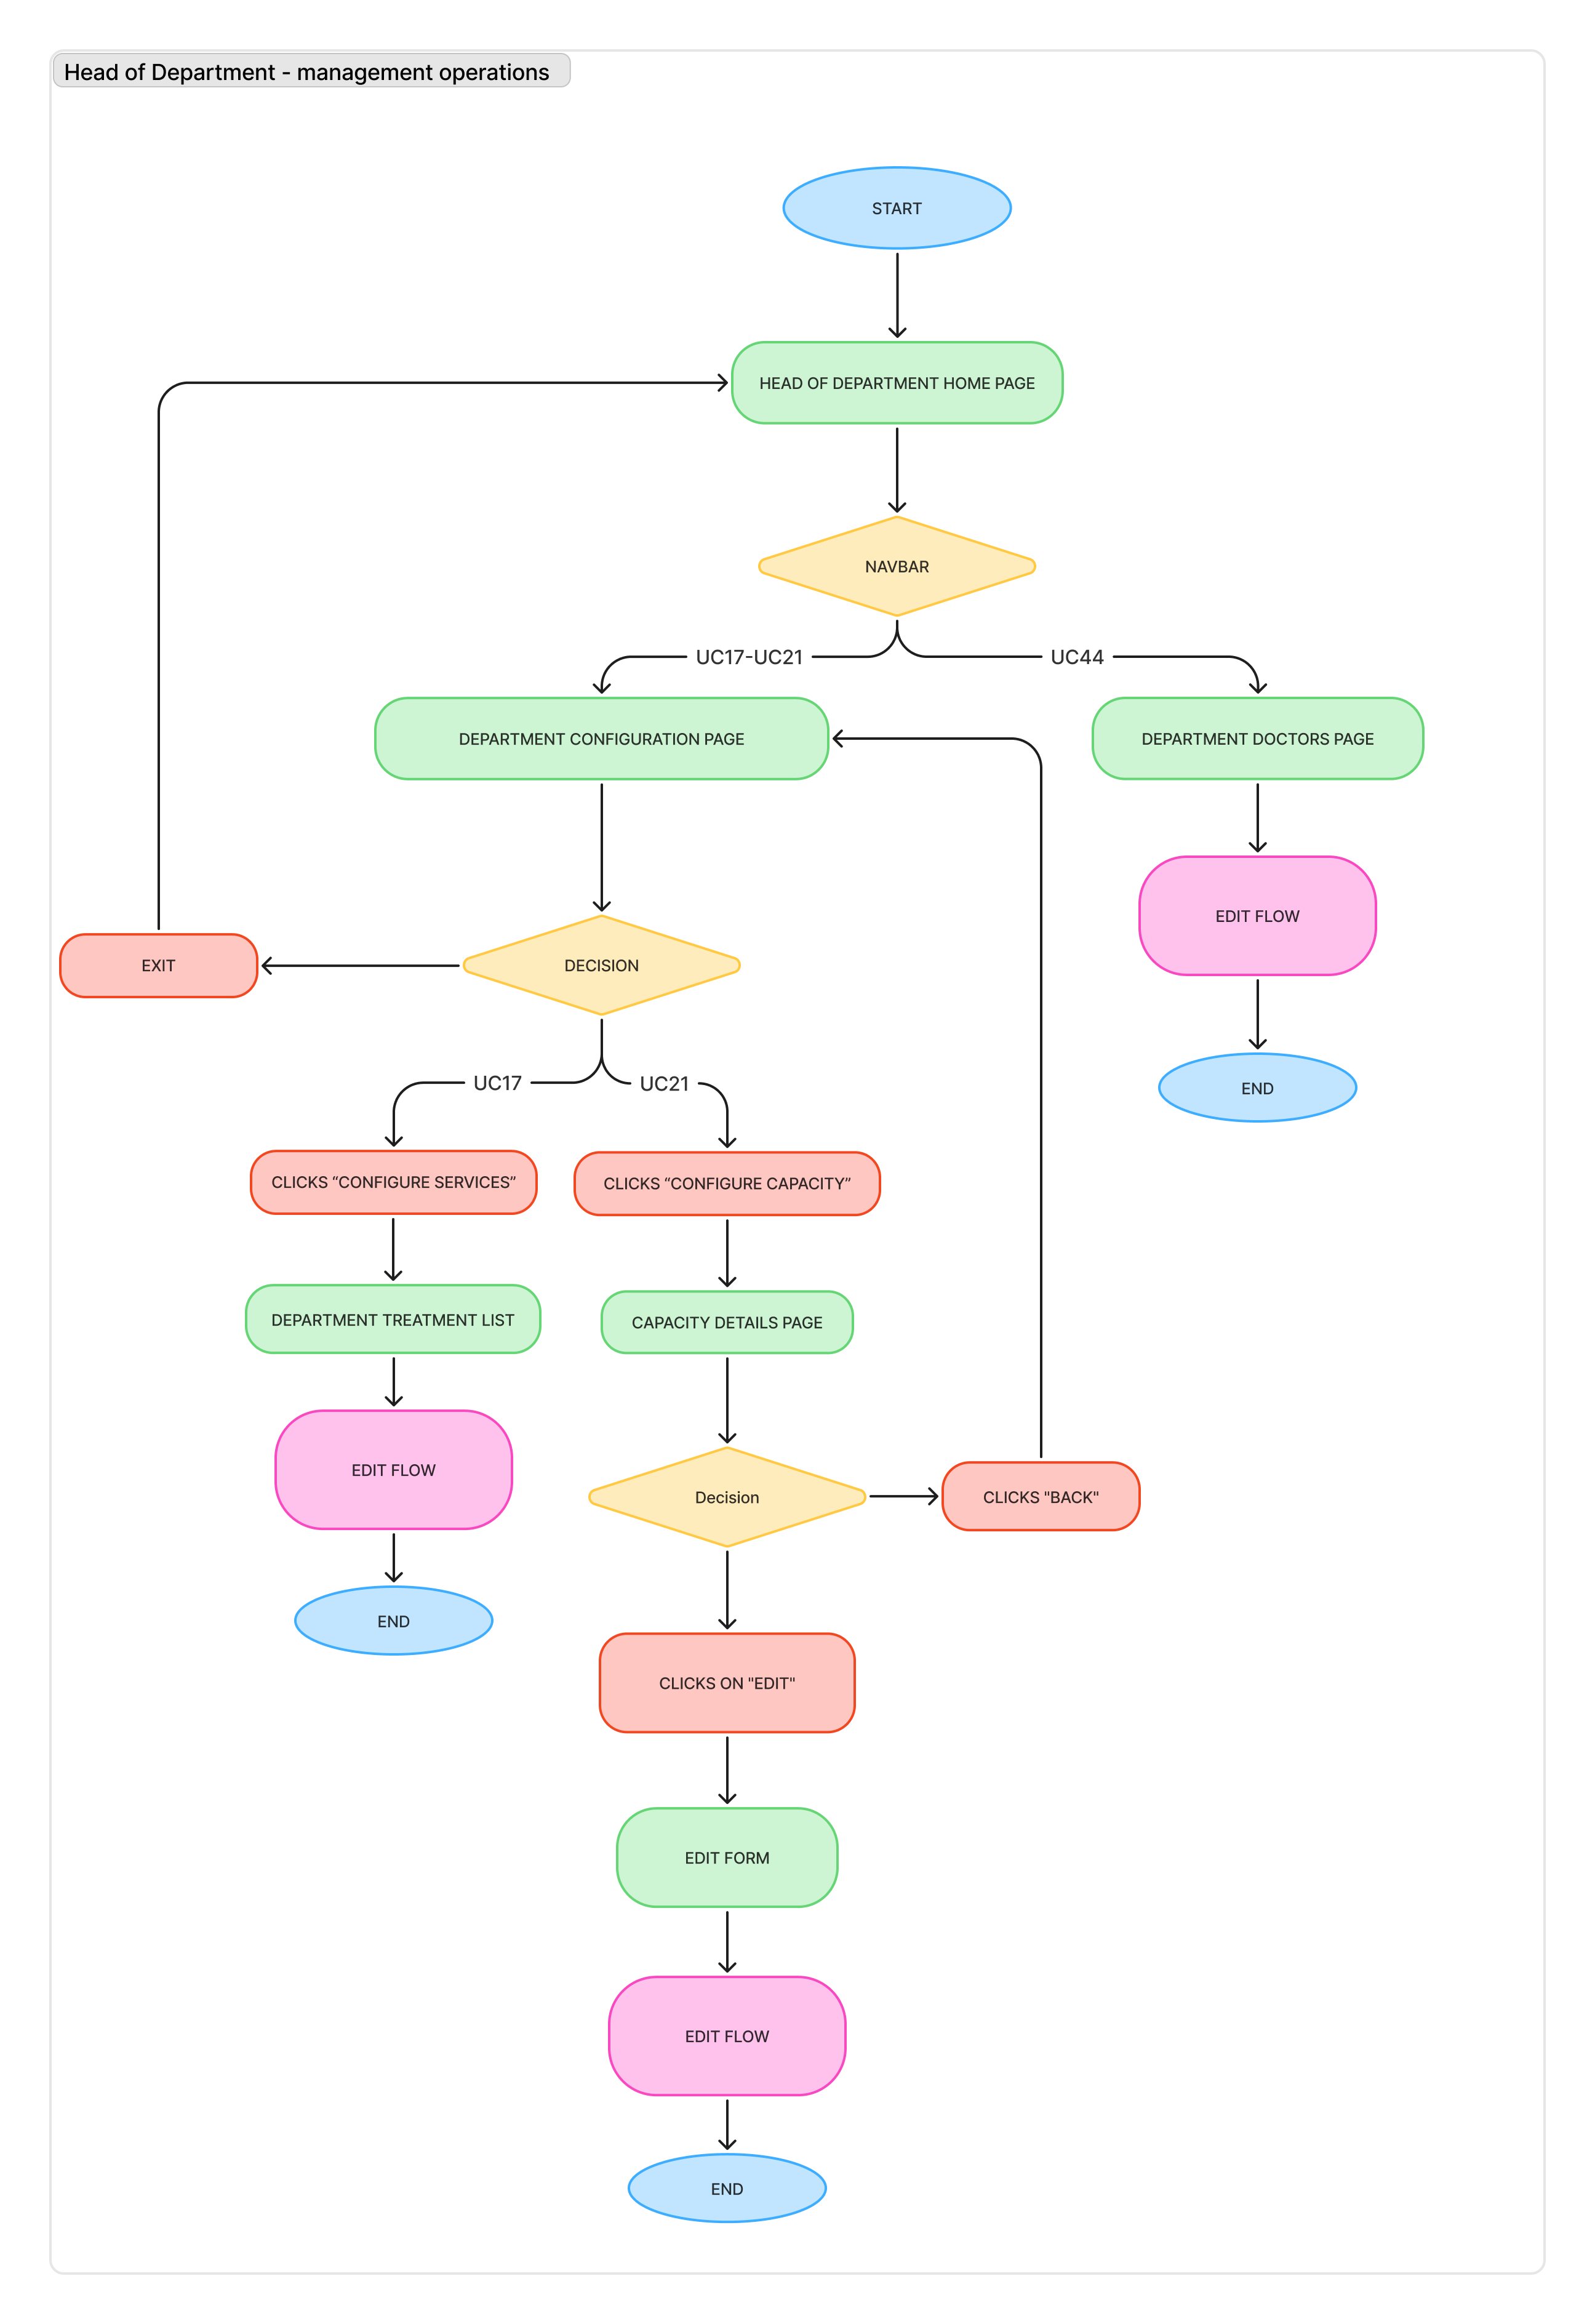
\includegraphics[width=0.9\textwidth]{User_Flows/DepartmentManagement.png}
        \captionof{figure}{User flow regarding Head of Department Management Operations}
    \end{center}
    %\begin{itemize}   
    %\end{itemize}
\end{minipage}
\vspace{3em}

\begin{minipage}{\textwidth}
    \phantomsection
    \subsection{UF21. Head of Department - Cancel Department Appointments}
    The following user flow shows the steps a head of department takes to cancel their department's booked appointments.
    It refers to use case \textbf{UC11}, and methods \textbf{cancelDepartmentAppointment(reason : String)} from the class \textbf{Head of Department} of the class diagram.
    
    \begin{center}
        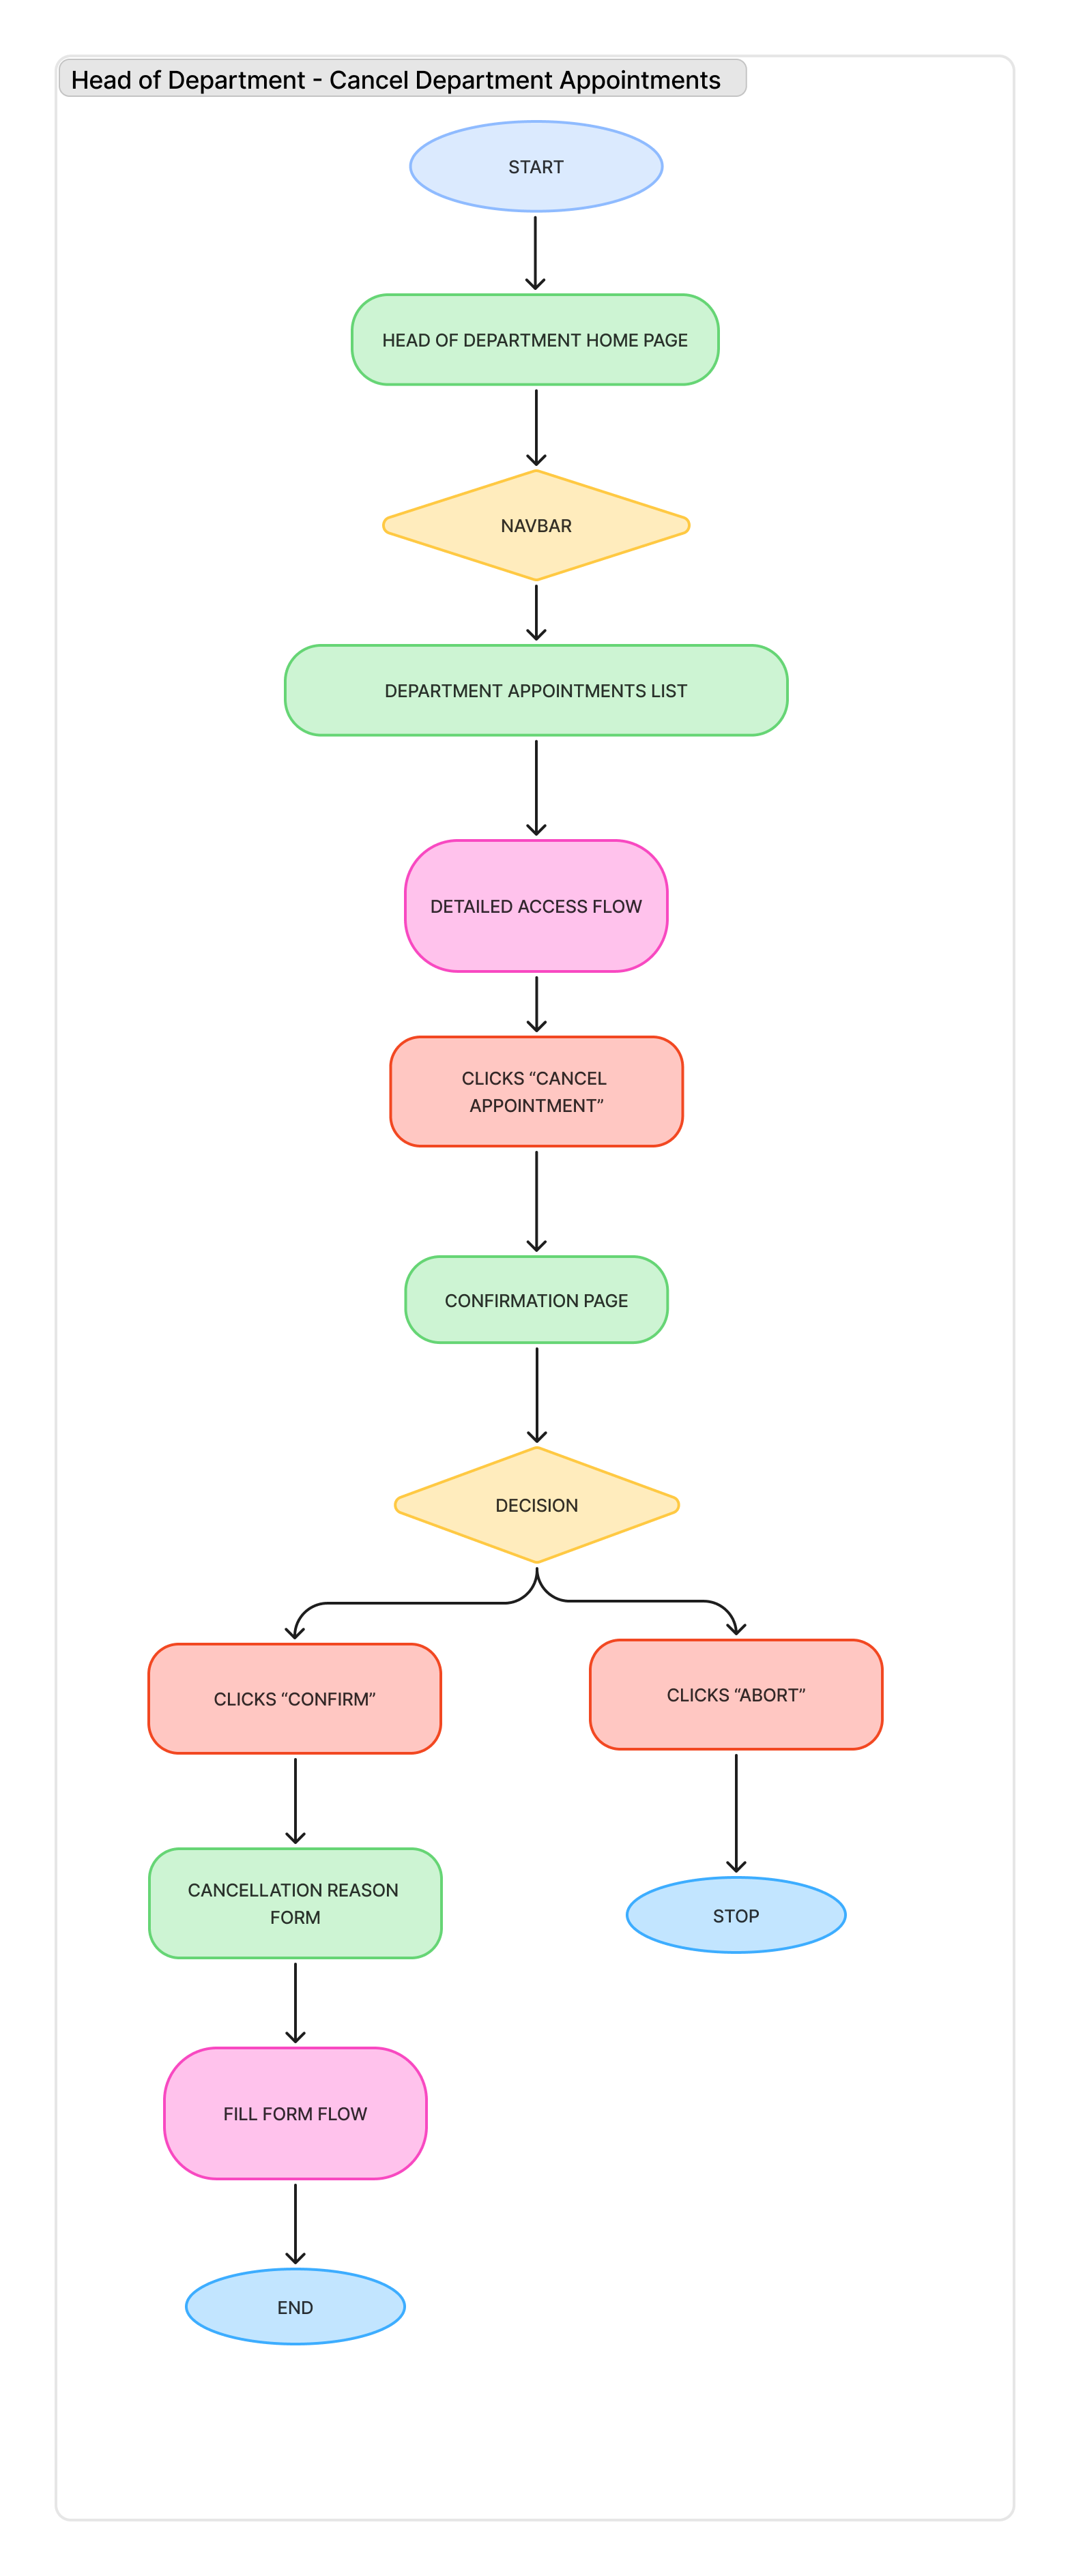
\includegraphics[width=0.9\textwidth]{User_Flows/DepartmentAppointmentCancellation.png}
        \captionof{figure}{User flow regarding Head of Department Cancel Department Appointments}
    \end{center}
    %\begin{itemize}   
    %\end{itemize}
\end{minipage}
\vspace{3em}

\begin{minipage}{\textwidth}
    \phantomsection
    \subsection{UF22. Head of Hospital - Insurances' Debt Management}
    The following user flow shows the steps a head of hospital takes to consult the insurances' debts owed to the hospital and register payments from insurance companies.
    It refers to use case \textbf{UC18, UC19, UC20}, and methods \textbf{viewInsuranceDebt(), settleInsuranceDebt(companyName : String, amount : Decimal)} from the class \textbf{Head of Hospital} of the class diagram.
    
    \begin{center}
        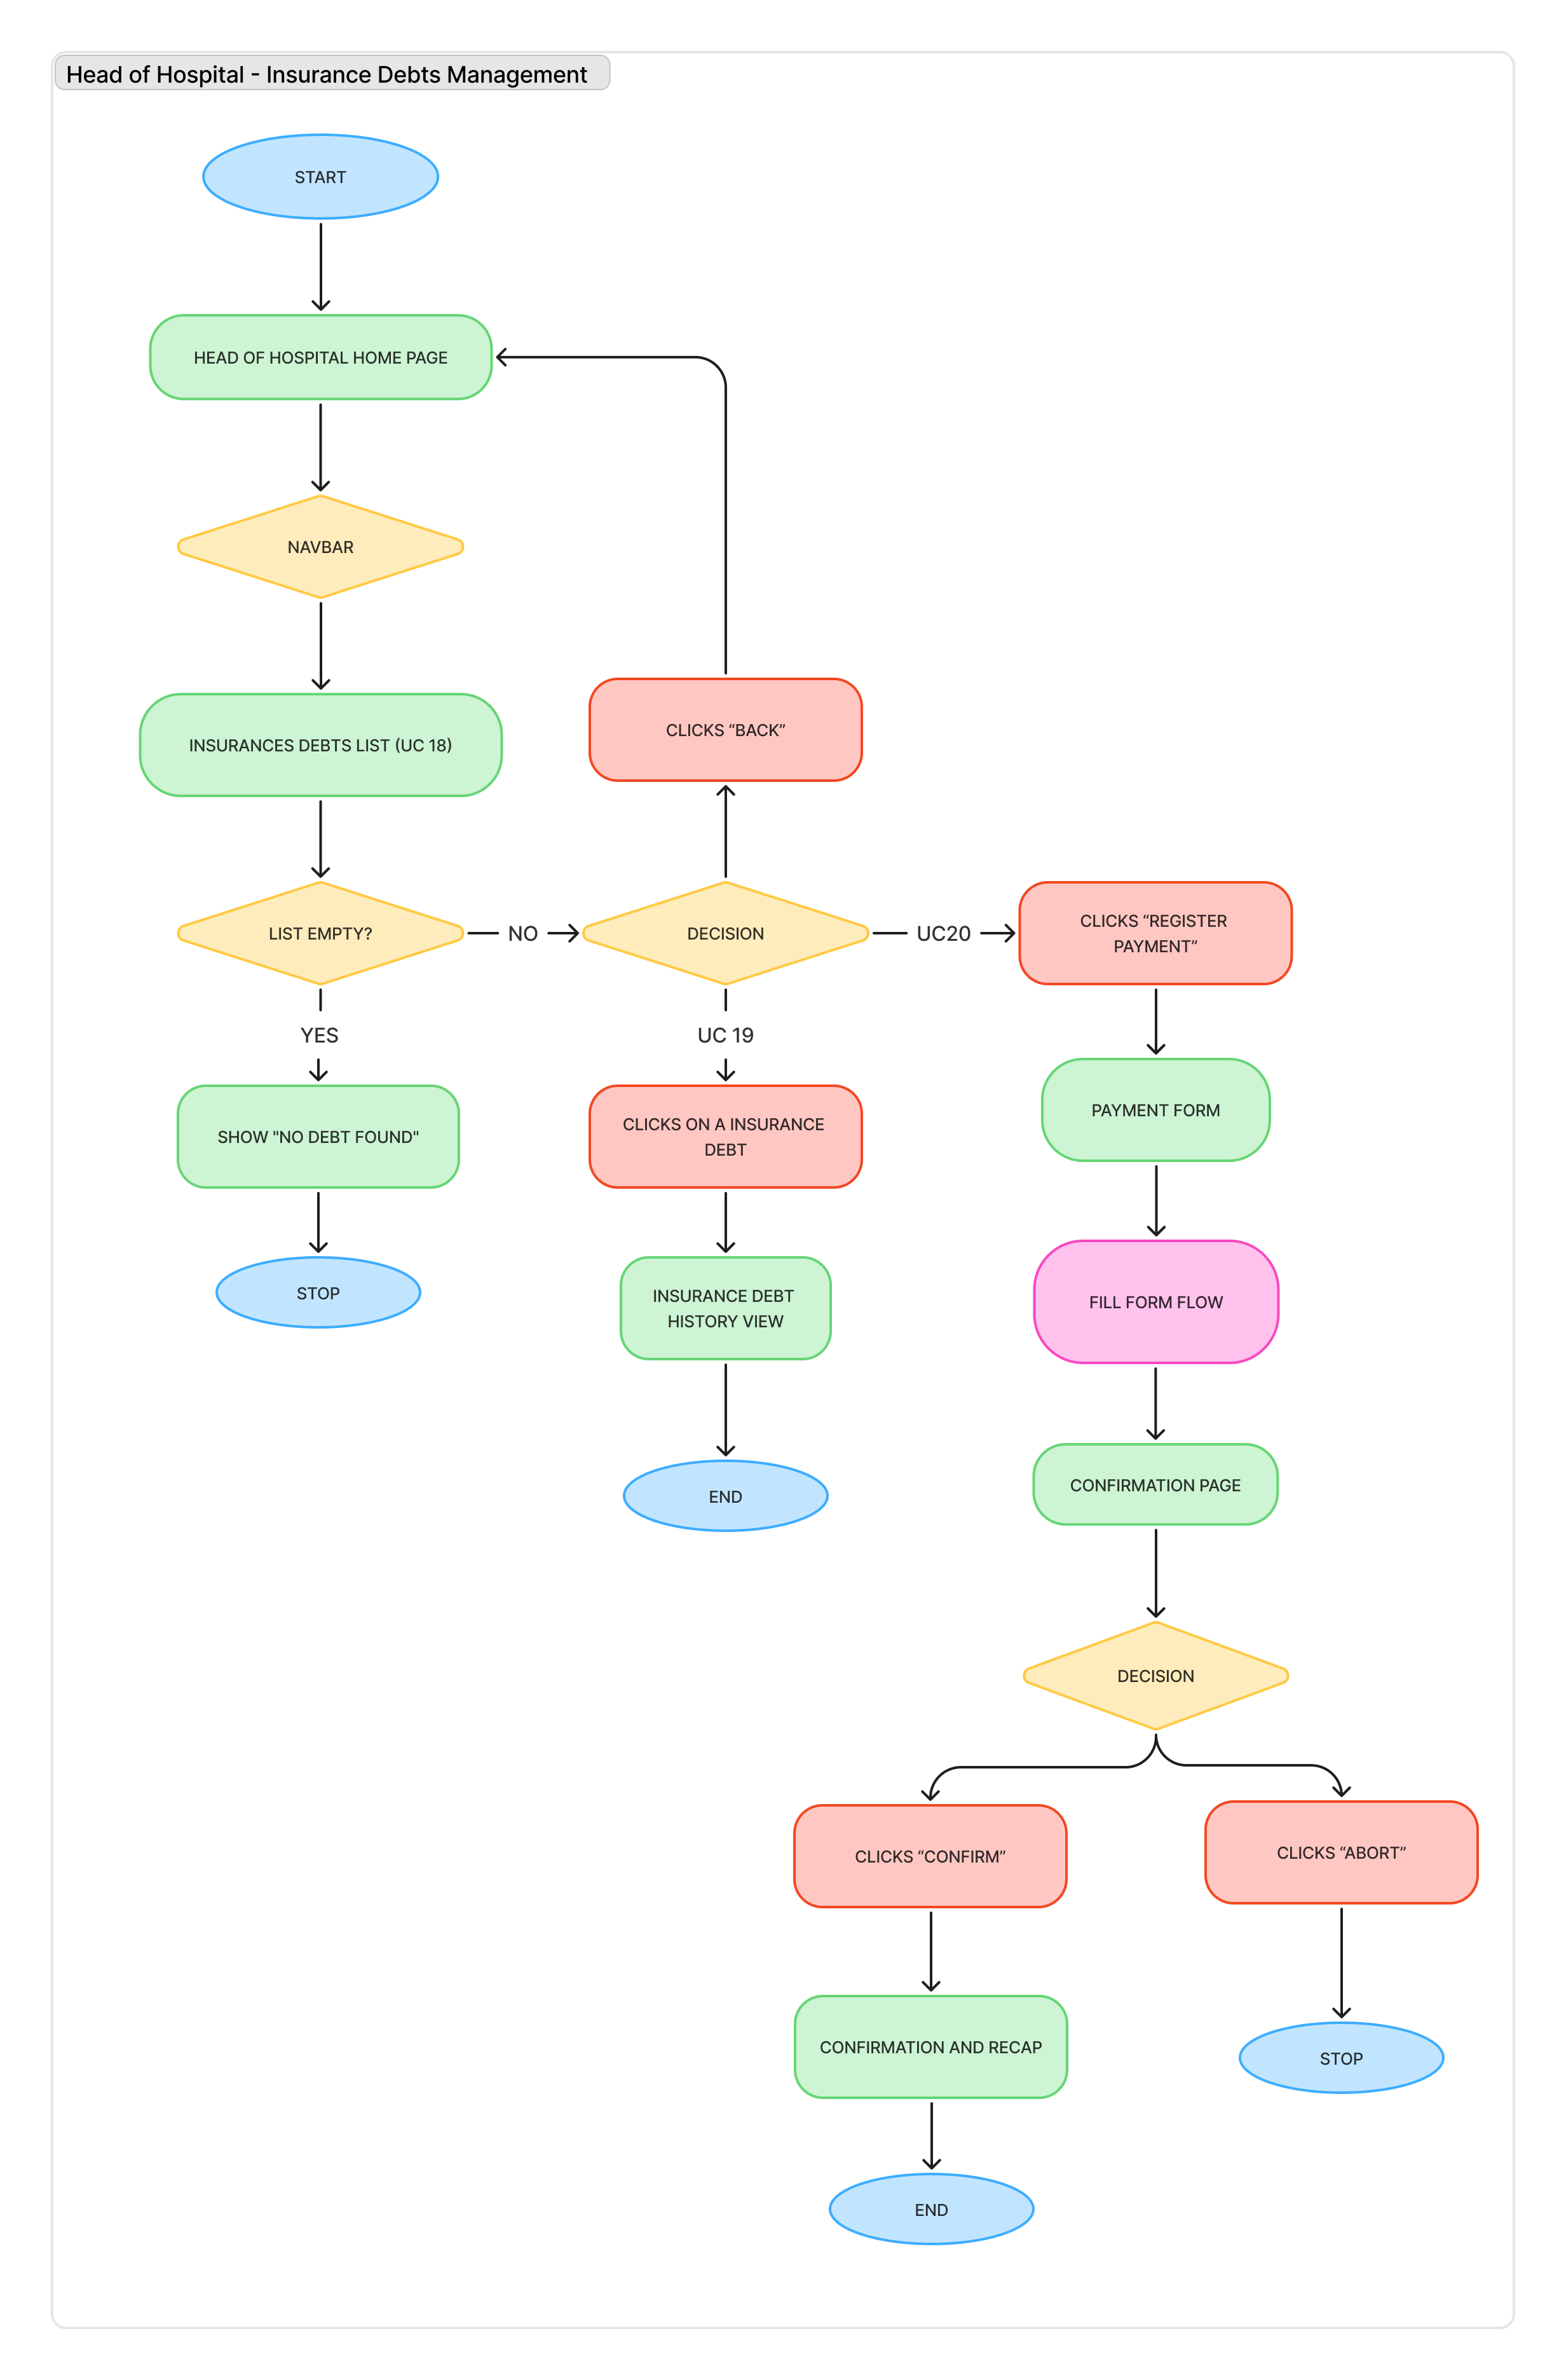
\includegraphics[width=0.9\textwidth]{User_Flows/HospitalDebtsManagement.png}
        \captionof{figure}{User flow regarding Head of Hospital Insurances' Debt Management}
    \end{center}
    %\begin{itemize}   
    %\end{itemize}
\end{minipage}
\vspace{3em}

\begin{minipage}{\textwidth}
    \phantomsection
    \subsection{UF23. Head of Hospital - Department Assignments Management}
    The following user flow shows the steps a head of hospital takes to appoint a head of department and assign a doctor to a specific department.
    It refers to use case \textbf{UC13, UC15}, and methods \textbf{appointHeadOfDepartment(doctor : Doctor, dept : Department), allocateDoctors(doctors : List<Doctor>, dept : Department)} from the class \textbf{Head of Hospital} of the class diagram.
    
    \begin{center}
        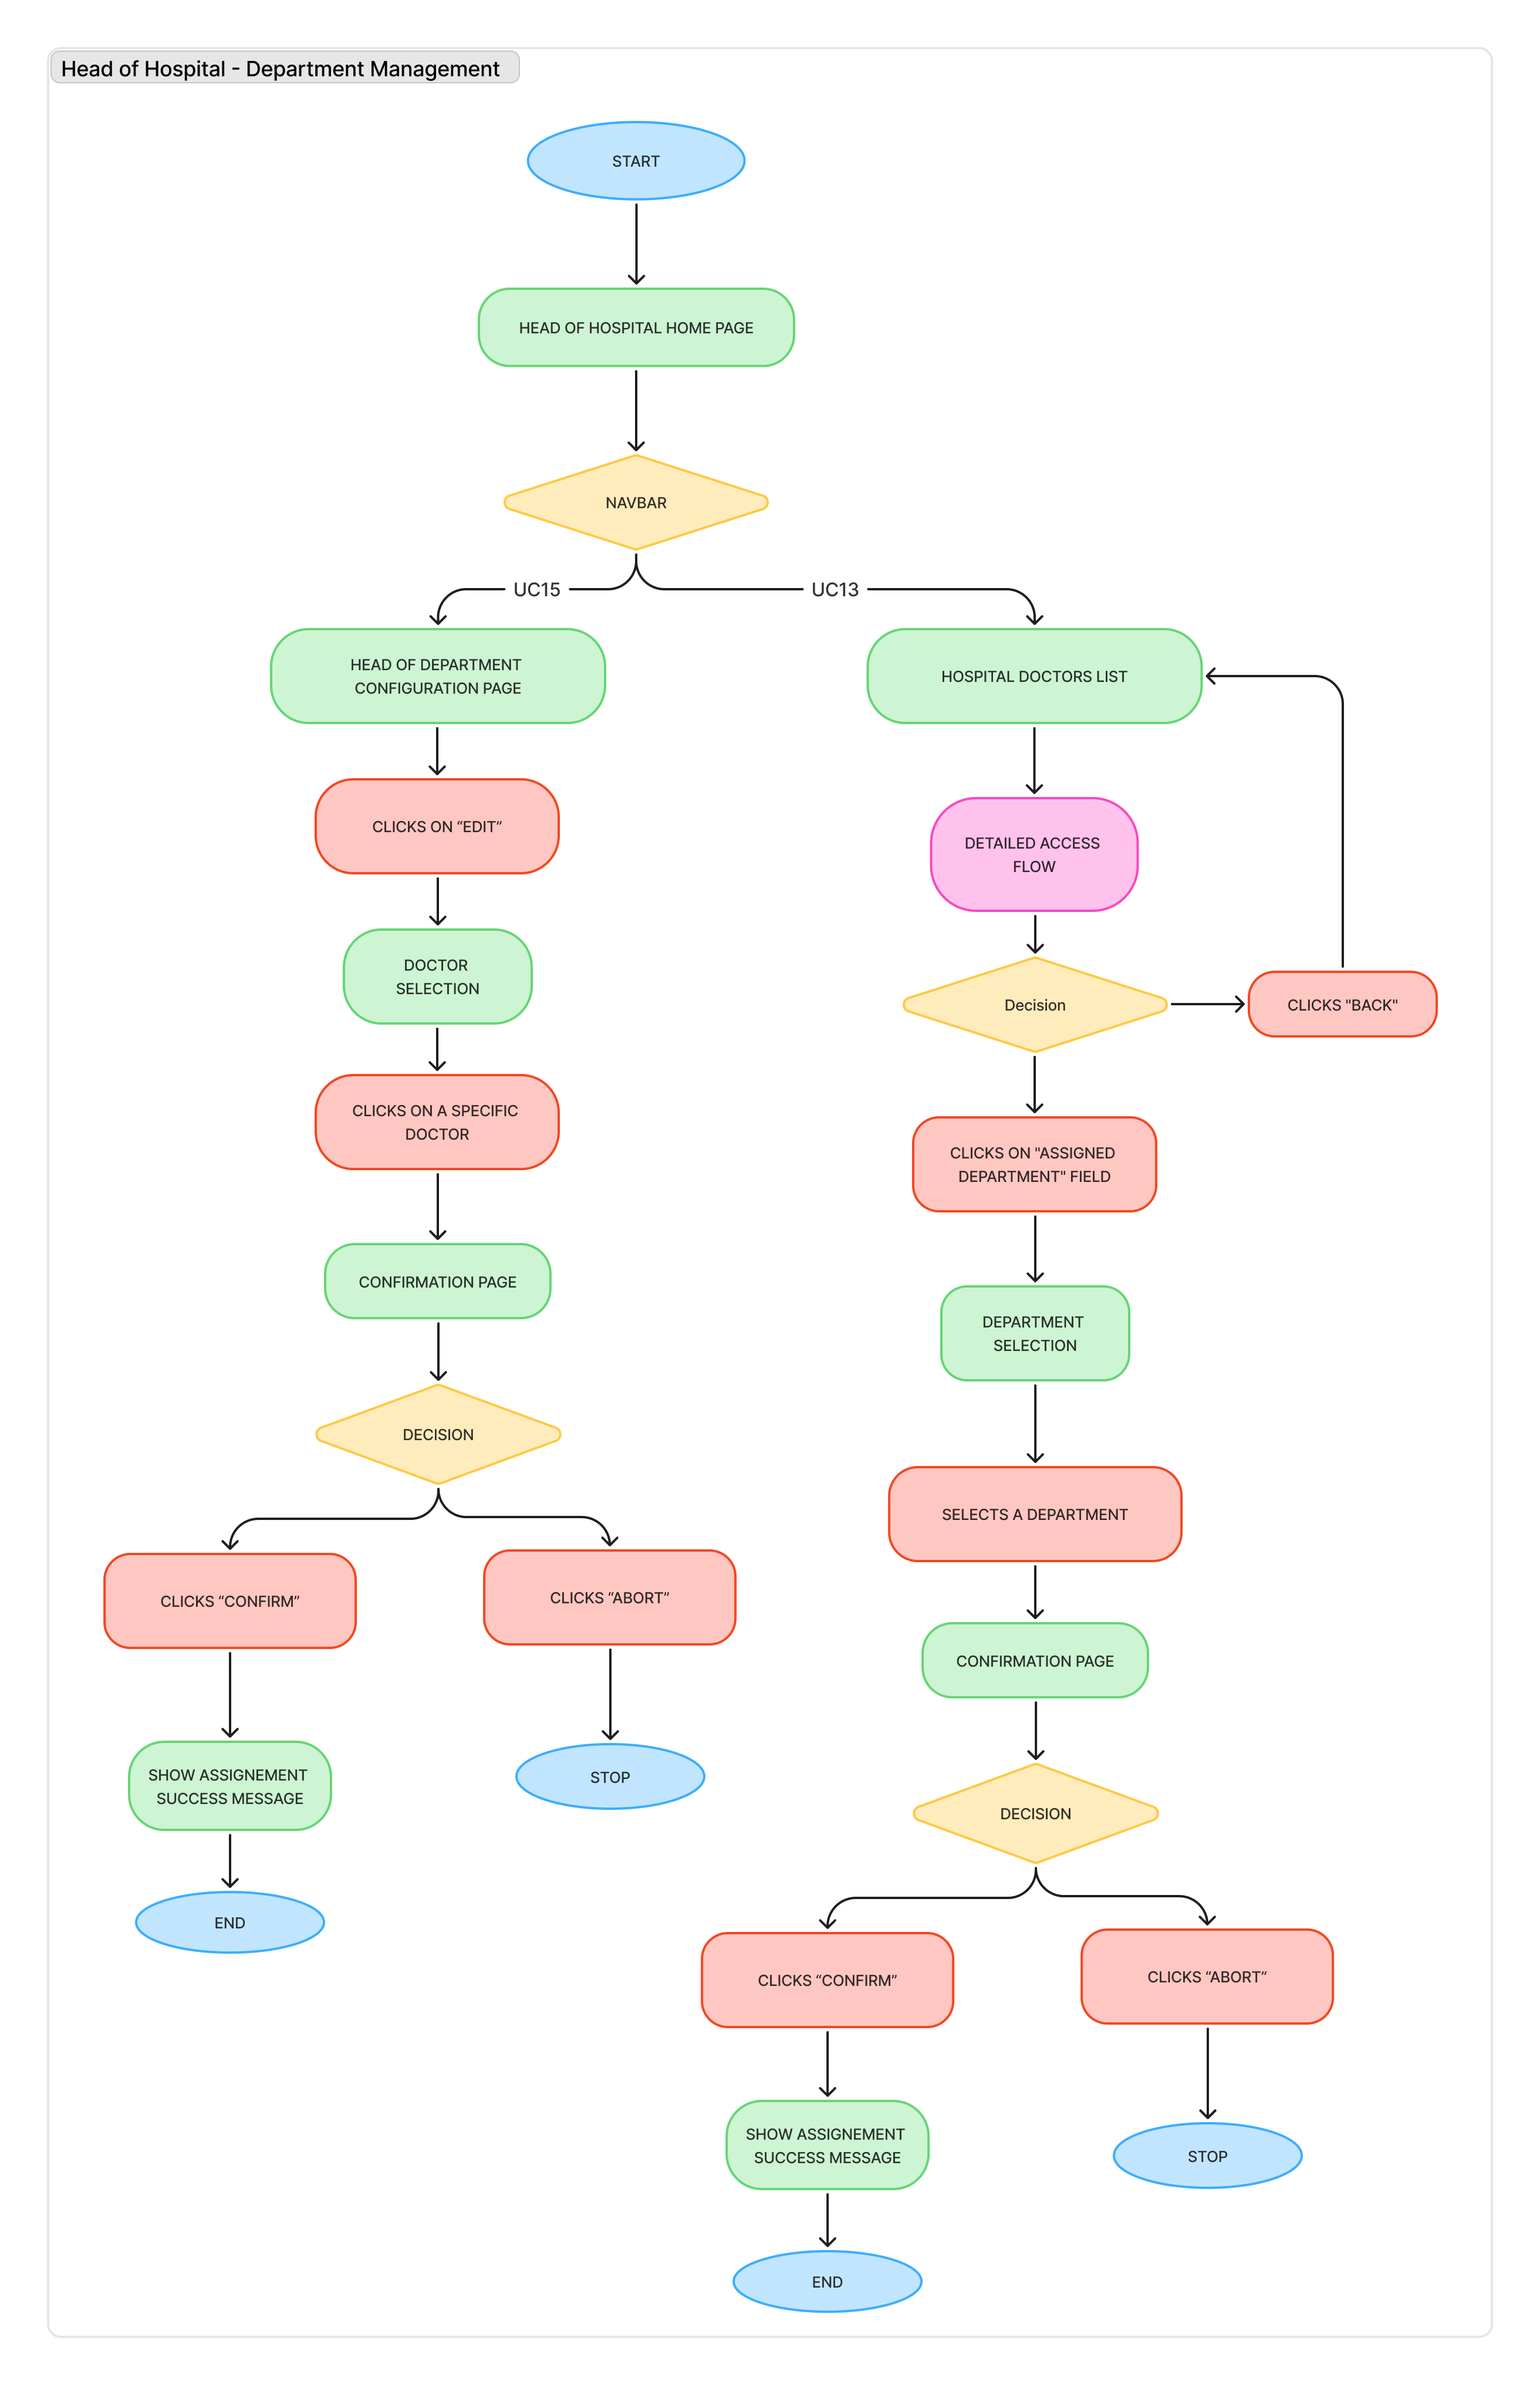
\includegraphics[width=0.9\textwidth]{User_Flows/HospitalHeadAssignements.png}
        \captionof{figure}{User flow regarding Head of Hospital Department Assignments Management}
    \end{center}
    %\begin{itemize}   
    %\end{itemize}
\end{minipage}
\vspace{3em}

\newpage
\phantomsection 
\section{Code Developement}
asdasdasd

\begin{minipage}{\textwidth}
    \phantomsection
    \subsection{1. Place holder}
    place holder!
    
    \begin{center}
        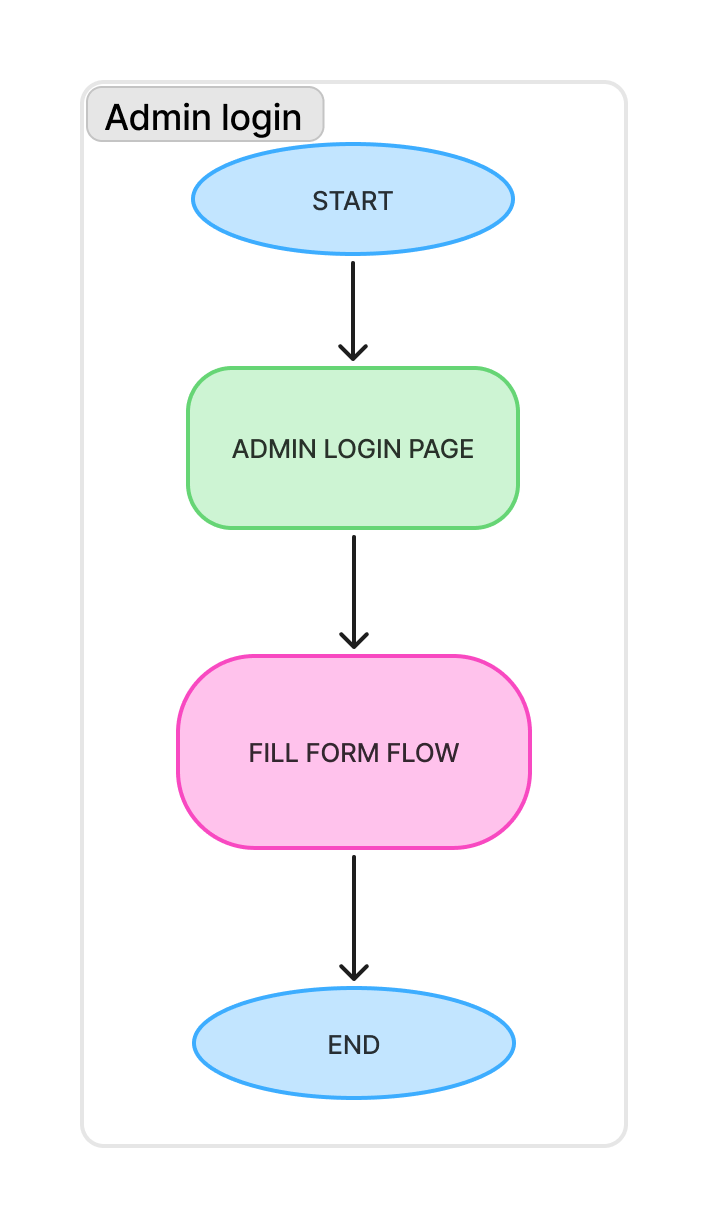
\includegraphics[width=5cm]{User_Flows/AdminLogin.png}
        \captionof{figure}{placeholder}
    \end{center}
    %\begin{itemize}   
    %\end{itemize}
\end{minipage}
\vspace{3em}

\phantomsection 
\section{Team Assessment}

\phantomsection 
\subsection{Work organization}

In the early stages of the project, the work was divided mainly according to:

\begin{itemize}
    \item equal division of the workload;
    \item assignment based on the basic skills that each person had;
    \item affinity for a specific task.
\end{itemize}

Maintaining the last two criteria mentioned above, it was subsequently decided to modify the first point by opting for a division of work based on the time available. To coordinate, we held weekly meetings either on Discord or in person. As the project progressed into the implementation and final phases, the frequency of meetings increased in order to better synchronize the work and address issues more promptly.

\phantomsection 
\subsection{Roles and activities}

\begin{table}[H]
\centering
\begin{tabular}{|p{2cm}|p{10cm}|}
\hline
\rowcolor{gray!50}
\textbf{Team Member} & \textbf{Main activities} \\
\hline
Stefano & Assigning and reviewing tasks, writing functional and non-functional requirements, writing use cases, front-end and back-end development \\
\hline
Federico & Proofreading of all deliverables: covering syntactic, logical, and grammatical inconsistencies, writing use cases, writing functional and non-functional requirements, creating user flows, creating the project boundary diagram \\
\hline
Giorge & Creating activity diagrams, creating sequence diagrams, writing functional and non-functional requirements, creating ER diagram, front-end and back-end development (minor contribution) \\
\hline
Luca & Creation of the class diagram, front-end and back-end development, defining requirements, defining architectural and language design choices, writing project objectives \\
\hline
\end{tabular}
\end{table}

\phantomsection 
\subsection{Workload and distribution}

Below is the workload expressed in percentage per deliverable for each member of the group.

\begin{table}[H]
\centering
\begin{tabular}{|p{3cm}|p{2cm}|p{2cm}|p{2cm}|p{2cm}|}
\hline
\rowcolor{gray!50}
 & \textbf{Stefano} & \textbf{Federico} & \textbf{Giorge} & \textbf{Luca} \\
\hline
D1 & 25 & 25 & 25 & 25 \\
\hline
D2 & 25 & 30 & 30 & 15 \\
\hline
D3 & 25 & 20 & 20 & 35 \\
\hline
\rowcolor{red!20}
\textbf{Proposed grade} & 30 & 30 & 30 & 30 \\
\hline
\end{tabular}
\end{table}

From the distribution of the participation described in the table, we can see that, except on the D1, the work was never perfectly balanced looking at the single deliverables. But indeed looking at it overall was performed equally by all members.

\end{document}
